
%%%%%%%%%%%%%%%%%%%%%%%%%%%%%%%%%%%%%%%%%%%%%%%%%%%%%%%%%%%%%%%%%%%%%%
\documentclass[promaster]{hdu-thesis}
\usepackage{xcolor}
\usepackage{array}
\usepackage{makecell} % 用于表头加粗
\usepackage{booktabs}
\usepackage{multirow}

% \usepackage{amsmath}  % 用于数学符号

\title{复杂动态环境下机器人导航系统设计与应用}{Design and Application of a Robot Navigation System in Complex Dynamic Environments}
\author{任佳乐}{Jiale Ren}%%%%%%作者
\advisor{黄娜}{Na Huang}%%%%%%指导老师
\school{自动化学院}{School of Automation}%%%%学院
\major{控制工程}{Electronic Information}%%%%%%%%%%专业
\authornumber{242060256}{} %%%%%%学号
\authorclass{2120601} %%%%%%%%%班级（本科生填）
\completedate{2027}{5}{May}  %%%%%%设计完成时间
\authordirection{路径规划}{path-planning}%%%%研究方向前者对应中文方向，后者对应英文（研究生写）
\begin{document}


%%%%%%%%%%%%%%%%插入封面%%%%%%%%%%%
\makecover
%%%%%%%%%%%%%%%%插入原创性声明%%%%%%%%%
\makedeclaration
%%%%%%%%%%%%%%%中文摘要%%%%%%%%%%%%%%
	
\cnabstract
变电站是电力系统运行维护中的关键节点，其内部存在高电压、强电磁干扰、设备密集、通道狭窄以及动态障碍物等复杂因素。传统人工巡检和辅助作业方式在安全性、实时性和作业效率方面存在一定局限，引入具备自主感知、定位建图和路径规划能力的移动机器人，是提升变电站运维智能化水平的重要途径。围绕变电站运维场景下机器人自主导航的实际需求，本文开展面向变电站运维的搬运机器人导航系统设计与实现研究。

首先，本文分析了变电站运维机器人的功能需求，设计了由传感器模块、中央控制模块、底层运动控制模块和电源模块组成的机器人硬件平台，并结合激光雷达、双目相机等传感器构建环境感知与导航系统框架。在此基础上，介绍了机器人导航所需的坐标系变换、点云聚类等基础理论，为后续环境感知、地图构建和路径规划提供统一的数据表达基础。

其次，针对机器人在复杂动态环境中对障碍物实时感知的需求，本文设计了基于深度图像和点云数据融合的轻量级障碍物检测与跟踪方法。该方法结合U深度图检测器和DBSCAN点云检测器的检测结果，通过包围盒匹配与融合提升障碍物检测的鲁棒性；同时引入基于特征的数据关联、恒加速度运动模型和点云投票策略，对动态障碍物进行状态估计与识别。在地图构建方面，本文采用局部占用栅格更新为规划器提供可更新的环境约束。

最后，面向变电站场景中的复杂障碍分布和实时避障需求，本文设计了全局参考引导与局部滚动优化相结合的分层路径规划方法。全局层采用目标偏向RRT生成二维拓扑可行参考路径，并结合直连检查、线段碰撞检测、超时处理和路径平滑后验校验提高工程可用性；局部层构建学习增强MPC规划器，在承接障碍物边界和动态状态估计结果的基础上，引入点级障碍表示、动态预测点流和学习型距离特征，生成满足运动约束、平滑约束和避障要求的局部轨迹。同时，本文设计MPC直接速度输出接口，将滚动优化得到的首个最优控制量转换为全向底盘可执行的速度指令。

\cnkeyword{变电站运维，移动机器人，自主导航，环境感知，路径规划}


%%%%%%%%%%%%%%%英文摘要%%%%%%%%%%%%

\enabstract Substations are key nodes in the operation and maintenance of power systems. Their operating environments usually involve high voltage, strong electromagnetic interference, dense equipment layout, narrow passages, and dynamic obstacles. Traditional manual inspection and auxiliary operation methods have limitations in safety, real-time response, and operational efficiency. Introducing mobile robots with autonomous perception, localization, mapping, and path planning capabilities is therefore an important approach to improving the intelligence level of substation operation and maintenance. Focusing on the autonomous navigation requirements of robots in substation operation and maintenance scenarios, this thesis studies the design and implementation of a navigation system for a substation operation and maintenance robot.

First, this thesis analyzes the functional requirements of the robot and designs a hardware platform composed of a sensing module, a central control module, a low-level motion control module, and a power supply module. A navigation framework is then constructed using sensors such as LiDAR and binocular cameras. On this basis, coordinate transformation and point cloud clustering methods required for robot navigation are introduced, providing a unified data representation foundation for subsequent environment perception, mapping, and path planning.

Second, to meet the need for real-time obstacle perception in complex dynamic environments, this thesis designs a lightweight obstacle detection and tracking method based on the fusion of depth images and point cloud data. The method combines the results of a U-depth image detector and a DBSCAN point cloud detector, and improves detection robustness through bounding box matching and fusion. Feature-based data association, a constant-acceleration motion model, and a point cloud voting strategy are further introduced to estimate and identify dynamic obstacle states. For mapping, local occupancy grid updating and octree-based global map representation are adopted to provide updatable environmental constraints for the planner.

Finally, considering the complex obstacle distribution and real-time collision avoidance requirements in substations, this thesis designs a hierarchical path planning method combining global and local planning. At the global level, the RRT algorithm is used to generate feasible paths, while map complexity evaluation, goal-biased sampling, and timeout fallback mechanisms are introduced to improve search efficiency and robustness. At the local level, model predictive control is adopted to track the global path and generate local trajectories under static and dynamic obstacle constraints. In addition, the controller design and the NeuPAN planner are discussed, providing a basis for further navigation optimization in non-convex obstacle environments and complex dynamic scenarios.

\enkeyword{substation operation and maintenance, mobile robot, autonomous navigation, environment perception, path planning}


	


% \cnabstract

% \begin{center} 
%   {\sihao\bfseries 热爱生命}\\[3pt]

% \end{center} 


% \cnkeyword{Latex，热爱生命，汪国真}


% %%%%%%%%%%%%%%%英文摘要%%%%%%%%%%%%
% \enabstract

% The use of latex in terms of thesis's writing.
% \enkeyword{Latex, thesis}




%%%%%%%%%%%%图目录%%%%%%%%%%%%%%%%
%\figurelist
%%%%%%%%%%%%%%%%%%%

% %%%%%%%%%%%%表格目录%%%%%%%%%%%%%
%\tablelist

% %%%%%%%%%%缩略词列表%%%%%%%%
%\glossarylist
% %%%%%%%%%%%%目录%%%%%%%%%%%
\tableofcontents

% %%%%%%%%%%%%%%%%%%%%%%%%

%%%%%%%%%%%%%%%正文%%%%%%%%%%%%



\chapter{绪论}
\section{研究背景及意义}
电力系统的安全稳定运行是国家经济发展与能源安全的基石。伴随着“碳达峰、碳中和”目标向纵深推进以及新型电力系统建设全面提速，电网结构与运行模式发生深刻变革，对作为电能转换与分配核心节点的变电站的智能化运维水平提出了前所未有的要求。
然而，变电站内部环境充斥着高电压、强电磁场、密集金属构架、狭窄通道以及有害气体（六氟化硫）泄漏等固有风险因素，构成了一个作业难度大、安全风险高的典型工业场景。传统的、高度依赖人工完成的设备巡检\textsuperscript{\cite{10753839}}、状态核查、开关操作、仪表记录及
应急处置等核心运维任务，不仅效率面临瓶颈，更使运维人员长期暴露于触电、机械伤害、高空坠落等严重职业安全风险之中。这种高风险人工模式与国家不断提升的安全生产标准（国家能源局与原安监总局2014年联合发布并不断强化的《防止电力生产事
故的二十五项重点要求》）形成了尖锐矛盾，亟需通过技术革新实现“机器换人、人机协同”，从本质上提升作业安全水平。

国家宏观战略层面对于解决上述难题、推动能源行业智能化升级的决心清晰而坚定。2022年3月由国家发展改革委、国家能源局联合印发的《“十四五”现代能源体系规划》​，将能源基础设施的智能化改造与数字化转型列为重点任务，明确要求“提升电网智能化水平，构建智慧能源系统”。
更直接的指引来自于2023年3月国家能源局发布的《关于加快推进能源数字化智能化发展的若干意见》​，该文件特别强调要“推动机器人\textsuperscript{\cite{9832477}}、无人机等智能装备在电力巡检\textsuperscript{\cite{ZDHT202511062}}、设备操作、带电作业、应急救援\textsuperscript{\cite{HUJX202504006}}等场景的规模化应用”，
将智能作业装备的部署上升至行业发展的战略高度。同时，以2015年《中国制造2025》为起点、后续《智能制造发展规划》《“十四五”机器人产业发展规划》以及2023年1月工业和信息化部等十七部门联合印发的《“机器人+”应用行动实施方案》​​ 共同构成的制造业升级政策体系，
都将智能机器人定位为突破复杂环境应用的关键抓手，尤其强调在能源、电力等高安全要求领域深化“机器人+”应用，提升劳动生产率和作业安全性。政策红利的直接效应体现在电网企业的实际行动上：国家电网“数字赋能，提质增效”战略、南方电网公司2020年启动的“数字南网”蓝图，
均斥巨资推进智能变电站建设，并将自主移动作业机器人视为实现“无人值守”目标不可或缺的技术支撑，为辅助作业机器人的研发与落地提供了强大的内在驱动力。

尽管固定式在线监测设备与无人机巡视\textsuperscript{\cite{ZLXC202503030}}已在变电站得到推广，为宏观状态监控提供了有效补充，但它们对需要深度介入的精细作业任务表现出明显的局限性。例如，开关柜内部触头的烧蚀状况排查、
设备连接点毫米级的松动检测、保护屏柜内密集指示灯的精确识别、高压设备的安全操作指令执行、复杂空间内的接地线辅助挂拆、故障设备现场状态的近场取证等核心环节，都要求作业主体具备在复杂物理环境与强电磁干扰下可靠感知、自主移动与精准执行的能力。
当下部署的巡检机器人虽能执行既定路线的巡检任务，但在面对变电站这一独特“考场”时，其核心能力——特别是高鲁棒性的环境感知、复杂受限空间下的可靠导航定位\textsuperscript{\cite{10528290}}、以及适应非结构化场景的动态规划与精细目标识别能力\textsuperscript{\cite{8865560}}——仍显不足。
技术瓶颈具体表现在：传感器系统（如激光雷达在强反射金属环境中、可见光相机在暗光/强光/视觉纹理缺失场景下）易受强电磁干扰和环境复杂性影响，导致感知数据失真、不稳定，难以构建对环境动态变化的可靠理解；在卫星定位信号缺失（室内或受遮挡区）且结构极其复杂（金属多径反射严重）的环境中，
同时定位与地图构建（SLAM）\textsuperscript{\cite{10034242}}的精度和鲁棒性面临严峻挑战，易出现定位漂移甚至失效；对变电站内大量存在的外观相似度高、排列密集、目标微小、易被部分遮挡的关键设备元件（如绝缘子串、线夹类型、特定仪表状态指示器）的检测与识别准确性，
直接制约着后续操作的精度与安全性；而这些感知与定位的不确定性，进一步制约了机器人在狭窄、障碍物多变的通道内实现高效、安全自主通行的能力。

因此，聚焦于研发能够有效克服变电站严苛环境挑战、具备自主作业能力的智能辅助作业机器人，并将研究重心置于其核心使能技术——包括多源异构传感器（激光雷达、多光谱视觉、IMU、UWB等）在强干扰环境下的深度融合\textsuperscript{\cite{10086242}}与抗干扰处理方法、针对复杂结构化/半结构化室内外场景的无GNSS鲁棒导航与地图构建策略、
融合环境语义信息\textsuperscript{\cite{10856442}}的动态路径规划\textsuperscript{\cite{10005857}}与精确避障机制、以及面向高相似度电力设备的高精度、高实时性目标检测与语义理解模型——不仅是对国家政策导向的积极响应，更是破解行业瓶颈、引领技术升级的必然选择。其价值首先体现在对电力安全生产本质性提升的贡献上，通过替代或辅助人工进入高风险区域执行任务，大幅降低甚至消除触电、机械伤害等事故风险，
彻底落实“生命至上、本质安全”的法规要求。其次，在提升运行效率与经济效益方面，机器人的引入能够实现近乎全天候的自主监控\textsuperscript{\cite{7105029}}与部分程序化操作，显著提高巡检覆盖面和频次，缩短设备停运窗口，提升响应速度，降低人力成本。尤其重要的是，基于其强大的感知能力提供的更精确、更丰富的实时数据，可为设备状态的精准评估和预测性维护提供坚实支撑，
有效规避重大设备故障造成的直接经济损失与间接社会成本，推动变电站运维模式向智能化、无人化高级形态演进。再者，攻克变电站这一极具挑战性的应用场景，本身就是推动相关技术领域创新的催化剂。在强干扰环境下实现多模态感知\textsuperscript{\cite{8628711}}的有效融合、开发适应非结构化空间的鲁棒导航定位算法、构建适用于特定复杂工业目标的智能识别模型\textsuperscript{\cite{10835912}}等突破，其技术外溢效应显著，
可广泛应用于电厂、换流站、乃至石化、轨交等其他高危复杂工业环境的自动化作业中，助力国产高端智能装备自主创新能力的提升。最终，从支撑国家能源转型与发展战略的角度审视，变电站辅助作业机器人的成熟应用，是构建新型电力系统智能化、自动化运维体系的关键环节，为保障国家能源安全、推动能源生产消费革命、最终实现“双碳”宏伟目标提供了基础性的技术保障。

目前在国家政策的强效驱动下，结合电网企业智能化升级的现实需求与当前技术瓶颈的清晰认知，深入研究并系统解决变电站辅助作业机器人在环境感知\textsuperscript{\cite{6523836}}、自主决策、安全运行方面的关键科学问题与技术难点，具有明确的应用紧迫性、显著的经济社会价值、重要的技术创新意义以及服务国家战略的深层内涵。


\section{国内外研究现状}
移动机器人感知与规划技术已发展成为现代智能系统的核心驱动力，其本质是构
建一套从环境认知到行为决策的闭合智能环路。当前技术前沿正经历从分立模块
化设计向多模态协同智能的系统性跃迁，其核心驱动力在于传感器硬件的颠覆性
革新、跨域数据融合范式的重构​​，以及安全约束下自主决策能力的质变。对于变
电站运维机器人来说，其工作的主要目的是在特定环境中，通过机器人搭载的传
感器获取复杂环境信息，并基于环境信息进行环境感知与自主定位，最终实现自
主导航并确保能够有效避开障碍物区域\textsuperscript{\cite{9679713}}。由此可见，移动机器人控制的研究重点
主要集中在环境感知和路径规划两个关键环节。在环境感知方面，主要依赖于传
感器对周围环境进行探测和数据采集，随后采用特定的数据表示方法构建环境地
图。这一过程不仅要求环境模型能够精确反映实际环境的空间特征，还需要具备
对动态环境变化的实时更新能力。环境感知的有效性直接决定了机器人对环境信
息的感知质量，而路径规划则是在此基础上，通过对环境模型的分析处理，确定
需要访问的目标点位置，并实时规划避障策略，最终实现控制机器人安全平稳地
到达目标点进行作业。
基于上述分析，本节将从环境感知方法与路径规划方法两个维度，系统阐述当前
相关领域的研究进展与现状。
\subsection{移动机器人环境感知研究现状}
随着自动驾驶与智能制造的发展，移动机器人环境感知技术正经历从单一传感器依赖向多模态智能融合的范式转换。国际研究核心聚焦于解决三大共性难题：动态复杂场景的实时建模、极端环境下的感知鲁棒性​​，以及海量数据的高效智能处理。激光雷达作为三维空间感知的核心传感器，其技术演进呈现多线束与固态化并行路线。美国Velodyne公司2025年推出的HDL-3600固态激光雷达\textsuperscript{\cite{LI2025112972}}通过MEMS微振镜阵列将通道数提升至360线，角度分辨率达0.05°，并在强降雨条件下保持80\%的有效点云捕获率，但成本高达8000美元，限制大规模商业化应用。与之对比，速腾聚创研发的M3平台采用转镜式方案，在保持128线性能的同时将价格压缩至2000美元级，已装配于菜鸟物流AGV集群，但其抗震性能较差，难以适应工程机械等高振动场景。毫米波雷达\textsuperscript{\cite{10028086}}领域，德州仪器的AWR2944芯片集成4发4收MIMO架构，通过多普勒-角度联合估计\textsuperscript{\cite{7346780}}技术将运动物体轨迹预测精度提升至0.1m/s，不过金属密集环境中的多径反射问题仍导致很高的虚警率。

可见光视觉感知在近年取得颠覆性突破。以色列Mobileye的EyeQ6芯片搭载神经拟态计算架构，利用事件相机\textsuperscript{\cite{8288670}}毫秒级动态响应特性，在强逆光场景下仍能保持很高的车道线检测率，特斯拉FSD V12系统则采用纯视觉方案构建时空记忆网络\textsuperscript{\cite{8623233}}，不再依赖于传统的高精地图和导航数据，而是完全依靠车载摄像头和神经网络来识别道路和交通情况，通过隐式神经表征实现无高精地图的厘米级定位并做出相应的决策，但这依赖超2000万公里真实路况训练的万亿参数模型，初创企业难以复制。国内旷视科技研发的软硬一体化方案“慧影”在低照度场景表现突出，联合优化ISP图像处理器与Transformer\textsuperscript{\cite{9649842}}网络，在低光照度下大幅提高了传统方法的行人检测召回率，该技术已用于美团无人配送车系列，然而在雨雾天气下识别性能仍会有巨大衰减。

环境感知数据处理的创新呈算法与硬件协同演进态势。多传感器时空配准领域，为了在同步定位与地图构建（SLAM）任务中实现精确且鲁棒的位姿估计，Zhang\textsuperscript{\cite{9981107}}等人提出了一种名为FAST-LIVO的快速激光雷达-惯性-视觉里程计系统，该系统基于两个紧密耦合且直接里程计子系统：一个视觉里程计子系统和一个激光雷达-惯性子系统。激光雷达-惯性子系统子系统将新扫描的原始点注册到逐步构建的点云地图中，地图点附加了图像块，在视觉里程计子系统通过最小化直接光度误差来对齐新图像，而无需提取任何视觉特征。
Nguyen等人对于VSLAM框架提出了一种基于多个邻近姿态的“加权平均”的新型方法，在保持其定位精度的同时，计算从当前图像帧到先前邻近帧的相机姿态后，提供定位估计。利用相机运动引入了两种立体模式\textsuperscript{\cite{8556398}}：“静态立体”模式（通过左右相机的固定基线设置）以及“时间多视图立体”模式。同时在尺度估计步骤中，将视差图限制为时间多视图立体模式内的内点，大大降低了计算成本。
Cheng\textsuperscript{\cite{10475560}}等提出了一用于实现高精度和鲁棒的车辆定位，在前端使用激光雷达点云获取视觉特征的深度信息，同步的惯性测量单元测量值以松散耦合的方式输入到姿态估计模块中。在后端提出了两种关键策略来减少算法的计算量，平衡选择策略基于关键帧和滑动窗口算法\textsuperscript{\cite{9679713}}，而分类优化策略基于特征点和姿态估计辅助。与Fast-LIVO 算法相比，其算法在精度和鲁棒性方面均表现更优，且具有最佳实时性能。
环境精确重建也是SLAM系统的核心目标。然而，智能体的轨迹会显著影响估计精度。阿根廷学者Gimenez提出了一种使用不确定性地图（UM）对主动SLAM系统中的地图不确定性进行建模的新方法。UM利用概率分布来捕捉地图不确定性的空间分布，从而将不确定性前沿（UF）转化为关键勘探-开发目标和潜在停止的标准\textsuperscript{\cite{SANSONI2025105059}}。与依赖于特定SLAM系统设置的方法不同，该方法可兼容不同类型的传感器，同时还解决了探索规划和停止条件中的常见问题，使智能体能够自主探索开阔空间。

针对动态目标处理，Li\textsuperscript{\cite{9327342}}等人使用具有丰富环境信息和深度信息的密集点云映射取代了传统的激光映射和稀疏点云映射，为了解决动态环境中运动物体的鬼影问题，引入Mask R-CNN来提取输入帧中的运动物体掩码。在定位精度满足要求后，提出了一种鲁棒的掩码截断符号距离函数模型，用于在动态室内环境中构建密集地图，通过体素的截断距离识别重置动态体素，然后更新密集点云映射。
Andrey\textsuperscript{\cite{10168408}}等提出了一种提高动态环境下地面移动机器人视觉惯性里程计鲁棒性的新方法，通过交替因子图优化扩展了标准视觉惯性导航系统，并使用加权最小二乘\textsuperscript{\cite{8996235}}状态估计问题。同时，基于场景的语义先验知识建立了视觉地标的可靠性模型，在高动态环境下实现了稳定和准确的状态估计。
为了解决动态场景中视觉同步定位与地图构建算法在相机位姿计算过程中常错误地包含动态点，导致精度和鲁棒性下降的问题，Yin\textsuperscript{\cite{YIN20251329}}等提出了一种基于目标检测和区域动态概率的动态SLAM算法。采用 YOLOX 目标检测模型获取二维语义信息并补偿漏检。接着通过聚类算法自适应地确定提取动态对象轮廓作为动态点的阈值，将图像划分为低动态、可疑动态和高动态区域。在跟踪线程中，动态点移除模块为这些区域中的特征点分配动态概率权重。结合几何方法，检测并移除动态点。该动态 SLAM 算法超越了大多数现有 SLAM 算法，在动态环境中提供了更好的位姿估计精度和鲁棒性。
在动态环境视觉同步定位与地图构建方面，Liu\textsuperscript{\cite{9497091}}等人提出了RDMO-SLAM方法，通过添加使用密集光流进行语义标签预测，能够在确保实时性的同时利用更多语义信息。同时估计每个地标的速度，使用其作为约束来减少动态物体在跟踪中的影响，该方法在保持动态场景中稳健跟踪的同时，将实时性能从15Hz提升至30Hz。
还有学者提出了一种通用的动态驾驶环境的参数化表示方法\textsuperscript{\cite{7271102}}，该方法基于常见的占用栅格地图环境表示，通过交互式多模型无迹卡尔曼概率数据关联（IMM-UK-PDA）滤波器以基于对象的方式同时提取、分类和跟踪属于动态对象的单元，并将其从栅格中清除。剩余的静态环境栅格随后通过图像分析领域的方法进行处理，然后通过基于信息滤波的自由空间边界轮廓跟踪创建时空平滑的紧凑参数化自由空间（PFS）地图，该方法具备紧凑性、静态与动态实体之间固有的协调性、无关细节的抑制，以及其传感器实时生成能力。

极端环境感知是近年攻关焦点。针对浓雾场景，卡耐基梅隆大学开发的FogNet网络融合透射率物理模型与深度学习，在能见度低于10m条件下将障碍物检出率提升至84\%。
Paloma等人提出了一种基于特征的3D映射方法，用于获取半结构化环境（如部分损毁的建筑）的紧凑模型，以便移动机器人在救援活动中使用。为了收集3D数据，采用安装在真实和模拟机器人上的摆动数据采集系统\textsuperscript{\cite{5354363}}。采用的分割算法源于计算机视觉技术的集成，能够快速分离对应于不同表面的点，通过对每个区域内的点进行最小二乘拟合并提取几何特征，基于扩展卡尔曼滤波器\textsuperscript{\cite{9117536}}的增量概率最大算法提供6D定位，并生成具有凸包表示的平面块地图。
Xing\textsuperscript{\cite{8822727}}等设计了一款配备尖端导航系统（激光雷达和雷达）以及新型气体探测能力（FireNose）的探索机器人，专为消防员定制，将传感器数据与实时二维地图相结合，通过传感器和数据处理方法的融合，提供清晰且用户友好的危险指示，形成全面的救援机器人，在消防领域具有不错的应用前景。
对于只依靠视觉感知的移动机器人来说，在经典的视觉伺服范式中，非完整移动机器人的视觉控制变得具有挑战性，这主要是由于运动和能见度限制，这使得机器人无法在不丢失相机视野中的基本视觉信息的条件下，达到指定位姿。Crombez\textsuperscript{\cite{SOUALHI2025104920}}等提出一种新的深度强化学习框架来解决非完整移动机器人的视觉伺服问题，该框架集成了深度递归策略、内在动机和一种新的辅助任务，利用经典视觉伺服方法的核心交互矩阵来解决非完整机器人系统的基于视觉的控制问题。

随着相关产业技术的发展，移动机器人环境感知技术已从“单一器件性能提升”转入“系统级智能融合”阶段。这一变革的核心在于感知系统正逐步演化为具备自主协同决策能力的有机整体，当前前沿研究不再局限于传感器个体的抗扰性增强或分辨率突破，而是转向构建跨模态感知\textsuperscript{\cite{CHEN2025103278}}\textsuperscript{\cite{LI2025152}}—边缘计算—场景认知闭环​​的综合技术生态。


\subsection{移动机器人路径规划研究现状}

移动机器人路径规划技术已从早期单一的静态环境避障，发展至当今动态复杂场景下的智能决策系统，其演进过程深刻反映了人工智能、控制理论及高性能计算的跨学科融合。在技术发展初期（2000-2010年），基于图搜索的传统算法如A*\textsuperscript{\cite{ZHANG2025103711}}、Dijkstra\textsuperscript{\cite{9019345}}主导了结构化环境中的路径求解，这些方法通过栅格化地图将连续空间离散化，虽能保证最优路径却受限于计算复杂度，难以应对实时性要求。随后采样式规划算法掀起革新浪潮：快速随机扩展树（RRT）及其优化版本RRT*通过概率采样突破维度灾难，将高维空间求解时间压缩一半以上。同期出现的人工势场法能实现毫秒级响应，却因局部极小点问题造成较高的规划失败率，凸显早期技术对环境动态性的适应不足。

环境复杂度的提升倒逼规划技术向多层级架构演进。2015年后出现的分层规划框架将任务解耦为全局路径生成与局部轨迹优化：全局层采用改进A*算法融合地形代价，结合运动学约束生成可达性路径；局部层则依赖模型预测控制（MPC）实现动态避障。研究人员提出利用模型预测控制在局部偏离规定的全局路径以响应动态环境\textsuperscript{\cite{10598326}}，为了确保局部路径和全局路径之间的一致性，对于不同起点和终点的路径引入了本地同位路径的概念，通过制定一个硬约束来确保局部路径与给定的全局路径一致。真正推动质变的是安全约束理论的工程化应用——控制屏障函数\textsuperscript{\cite{10886491}}\textsuperscript{\cite{MURAMATSU2024114}}（CBF）的提出，通过微分不等式构建安全空间，确保机器人轨迹始终满足速度、加速度等物理约束，该技术已成为当前安全标准的理论基石。

受自然界生物行为启发，诸如蚁群算法\textsuperscript{\cite{11018948}}、遗传算法\textsuperscript{\cite{10151834}}等智能进化算法也逐渐运用到路径规划中。Zhong\textsuperscript{\cite{ZHONG2025111250}}等从果蝇行为中得到灵感，引入了一种新的采样器，该机制通过选择最佳采样候选策略或虚拟子目标点来优化双树采样过程。最优采样候选策略在三维空间进行全局采样，有效减少采样时间，虚拟子目标点加速了双树连接过程，增强了方向引导。使用果蝇机制重建了路径，从而降低了无人机路径成本。同时还提出利用Halton序列代替伪随机序列，从根本上解决了RRT方法中的欠采样和过采样问题。
受蛇类捕食行为启发，研究人员提出了蛇优化算法。原始SO在种群多样性和搜索精度方面仍存在不足，容易陷入局部最优。为此，研究人员又提出了改进蛇优化算法\textsuperscript{\cite{ZHU2025127660}}（ISO），通过引入三种全新的增强策略，显著提升算法性能。ISO 模拟了蛇类在自然环境中应对捕食与生存压力的多样化行为：初始化阶段采用多策略混沌系统，增强个体初始分布的随机性与均匀性；探索阶段融合反捕食者策略，拓展搜索范围，提高收敛速度与精度；开发阶段引入双向种群进化动态，保持种群多样性，强化全局搜索能力与局部开发能力的平衡。


与此同时，深度学习驱动的方法开辟了新路径：端到端强化学习在仿真环境中训练策略网络。
Lai等为解决移动机器人轨迹规划的问题提出了一种强化学习范式，将隐式策略与 Lyapunov 理论相结合\textsuperscript{\cite{LAI2025113870}}，开发了一个加权不对称的Lyapunov奖励函数，并提供了一个以适度动力学作为隐含策略的解析解，提出了事件触发的多目标策略优化。这是一种根据事件触发条件动态调整优化目标的方法，缩小了探索空间，实现了RL策略的迭代改进。
Fu等提出了一种危险感知机器人导航算法\textsuperscript{\cite{10445747}}，通过定义行人的危险并引入有关参考路径的虚拟机器人。该算法的主要新颖之处在于，利用虚拟机器人来获得额外的动作和更多的采样航点，以追求机器人运动的平滑性和前瞻性。并且建立优先机制并将其纳入深度强化学习导航，以提高机器人导航的安全性。
Ho\textsuperscript{\cite{HO2025104008}}等提出了一种强化学习路径规划方法用于智能仓库或智能工厂内自动导引车的实时路径规划。与难以适应动态运营变化的传统路径规划方法不同，该算法集成了实时信息，以实现响应迅速且灵活的路径决策。通过将移动机器人路径规划和强化学习集成到动态环境中，例如包含各种工作站、充电站和存储位置的智能仓库。在处理复杂的物流和运营环境方面展现出了高效性。

当前路径规划技术瓶颈主要体现在两个方面​​：1、复杂动态环境中的长程规划容易陷入计算泥沼；2、多目标优化存在根本性矛盾。为了逐步解决上述问题，研究人员在过去几年做出了不懈努力。针对复杂和狭窄的工作空间，Yin\textsuperscript{\cite{YIN2025128625}}等对协作路径规划问题提出了一种改进的多任务约束多目标优化。采用具有动态约束松弛和混合差分进化算子的多任务协同进化框架。同时优化主辅任务，平衡全局勘探和本地开发。采用多涡叠加模型量化环境干扰，构建无人驾驶车辆路径规划模型，结合任务协作效率、威胁风险成本和能耗目标。
Jihoon等提出了一种用于室内搜救作业的多级路径规划系统\textsuperscript{\cite{10107604}}，对路径规划系统的要求是基于集成室内导航系统的作业概念得出的。提出了一个五步路径规划系统，该系统由地图预处理、路段路径规划、图形处理、路线优化和路径后处理组成，通过采用基于图的方法，以计算高效的方式解决了多层建筑中的多目标路径规划问题，同时满足预处理和后处理步骤中的间隙条件等要求。

综上所述，移动机器人路径规划是一个涉及多方面优化技术的问题，针对不同的
任务需求需进行特定优化。随着技术不断的发展，越来越多的跨学科知识被广泛
应用于路径规划的研究当中，并取得了一定的研究进展。以上研究在实际的应用
中仍存在计算量大、规划效率低或部署成本过高等问题。未来的研究应着重于提
高路径的搜索效率和路径质量，降低算法部署成本。同时提高算法的鲁棒性，特
别是在动态复杂环境中的应用。


\section{本文主要研究内容}

\begin{figure}[!htb]
    \centering
    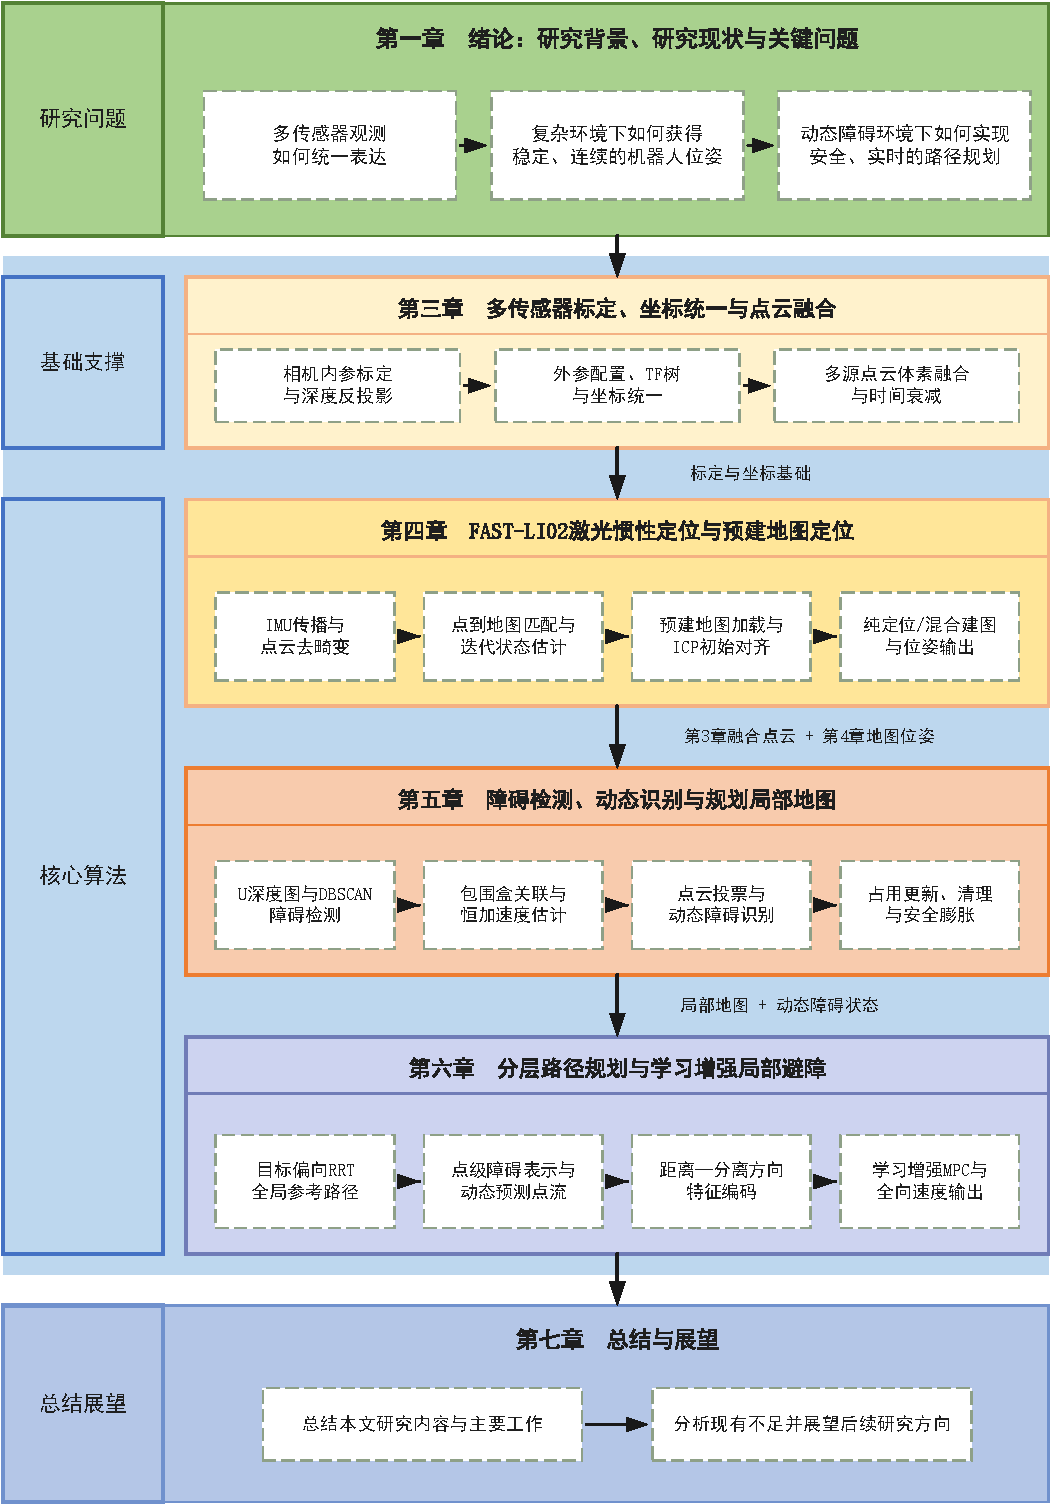
\includegraphics[width=\textwidth]{pic/论文框架图.pdf}
    \caption{本文研究内容与技术路线框架}
    \label{fig:论文框架图}
\end{figure}

围绕变电站运维搬运机器人在复杂、受限和动态环境中的自主导航需求，本文重点研究多传感器数据处理、激光惯性定位、障碍物检测与跟踪以及分层路径规划等关键问题，具体研究内容如下。

第三章阐述了多传感器标定与坐标变换方法。首先，定义了世界坐标系、机器人基坐标系、激光雷达坐标系和相机坐标系，并建立了各坐标系之间的齐次变换关系；其次，针对双目深度相机介绍了针孔成像模型、镜头畸变模型和张正友标定法，并完成了Gemini335L深度相机红外图像流的内参标定；然后，结合传感器的机械安装关系配置激光雷达、深度相机与机器人基坐标系之间的静态外参及TF变换；最后，研究了深度图像反投影、点云坐标变换以及多传感器点云融合方法，采用局部体素地图对激光雷达和深度相机观测进行统一表达，并通过差异化融合和时间衰减机制为后续障碍物检测与路径规划提供稳定的局部环境观测。

第四章研究了基于FAST\_LIO2的激光里程计定位方法。首先分析了激光雷达与惯性测量单元紧耦合定位的基本原理，介绍了IMU状态传播、点云去畸变、直接点到地图匹配、迭代误差状态卡尔曼滤波以及基于ikd-Tree的增量地图维护方法；在此基础上，面向变电站等具有预建地图的应用场景，设计了预建点云地图加载、地图降采样、初始位姿估计和ICP精配准相结合的定位初始化流程；进一步研究了固定预建地图下的纯定位模式和允许在线更新的混合建图模式，明确了定位系统向上层感知和规划模块输出全局位姿、连续轨迹及当前帧点云的接口，为机器人在复杂环境中的稳定定位提供基础。

第五章研究了运维机器人障碍检测与环境感知方法。针对小型移动机器人计算资源有限、深度相机视场受限以及复杂环境中单一传感器容易误检的问题，构建了基于深度图像和点云数据融合的轻量级障碍物检测与跟踪框架。首先介绍了K-Means和DBSCAN点云聚类方法，并分别利用U深度图检测器和DBSCAN检测器提取障碍物信息；随后对不同检测器的结果进行关联与融合，结合包围盒运动状态、点云运动一致性和点云投票机制识别动态障碍物，并利用滤波方法估计障碍物的速度和加速度状态；最后，基于第3章输出的多传感器融合观测以及本章获得的障碍物检测与跟踪结果，研究障碍物检测后的局部地图更新、自由空间确认、陈旧占用清理和障碍物膨胀方法，构建面向路径规划安全约束的局部环境表示。

第六章研究了分层路径规划与学习增强局部避障方法。针对变电站环境中设备密集、通道狭窄、障碍物形状复杂以及动态障碍物持续变化等问题，构建了“全局参考引导—局部滚动优化—底盘速度执行”的分层规划框架。全局规划层采用目标偏向RRT生成二维拓扑可行的参考路径，并通过直连检查、线段碰撞检测、超时处理、路径裁剪、路径平滑及平滑后碰撞复检提高全局路径的工程可用性；局部规划层建立全向移动底盘运动模型，将第5章输出的障碍物边界点和动态状态估计结果转换为点级障碍表示及预测点流，并引入点级几何编码器学习障碍边界与机器人轮廓之间的距离和分离方向特征，在此基础上构建带误差补偿、控制约束和松弛变量的学习增强MPC；最后，设计了优化失败、求解超时、碰撞风险和目标到达等异常状态处理机制，将MPC输出的首个最优控制量直接映射为全向底盘的速度指令，并通过仿真与实物实验对规划方法的可行性和实时性进行验证。

综上，本文围绕机器人导航系统中的“传感器数据统一—机器人状态估计—环境障碍理解—路径规划与控制执行”这一技术链条展开研究，形成了从多源感知输入到全向底盘速度输出的导航算法体系。

\chapter{机器人系统框架总体设计}
\section{机器人功能需求分析}
对于面向变电站辅助作业的运维机器人，为满足其特殊应用场景对可靠性、高性能的综合要求结合其工作内容，要求机器人具备以下功能：
（1）具备环境感知模块，可通过传感器与周围环境进行信息交互，感知自身作业环境；
（2）具备实时处理复杂空间信息的能力，实现高精度环境地图构建，以及在动态环境中的厘米级自我定位。
（3）具备基于先验地图自主导航模块，导航过程中能够自主规划出从当前位置到目标点的最优全局路径。
（4）具备任务执行过程中的未知障碍物规避能力，即在遵循全局路径的同时，实时感知并绕开未预见的障碍，并在必要时触发路径重规划机制以应对复杂的突发状况。
\section{机器人系统方案设计}
针对第~2.1节提出的环境感知、定位建图、自主导航与动态避障四项功能需求，本文采用”感知--决策--执行”的分层模块化方案设计运维机器人系统。整体方案在逻辑上划分为感知层、决策层和执行层三个层次，在物理上对应传感器模块、中央控制模块、底层运动控制模块和电源模块四类硬件，并以中央控制模块为核心实现各层之间的数据流转与指令下发。系统总体方案如图~\ref{fig:系统总体方案}所示。

\begin{figure}[!htb]
	\centering
	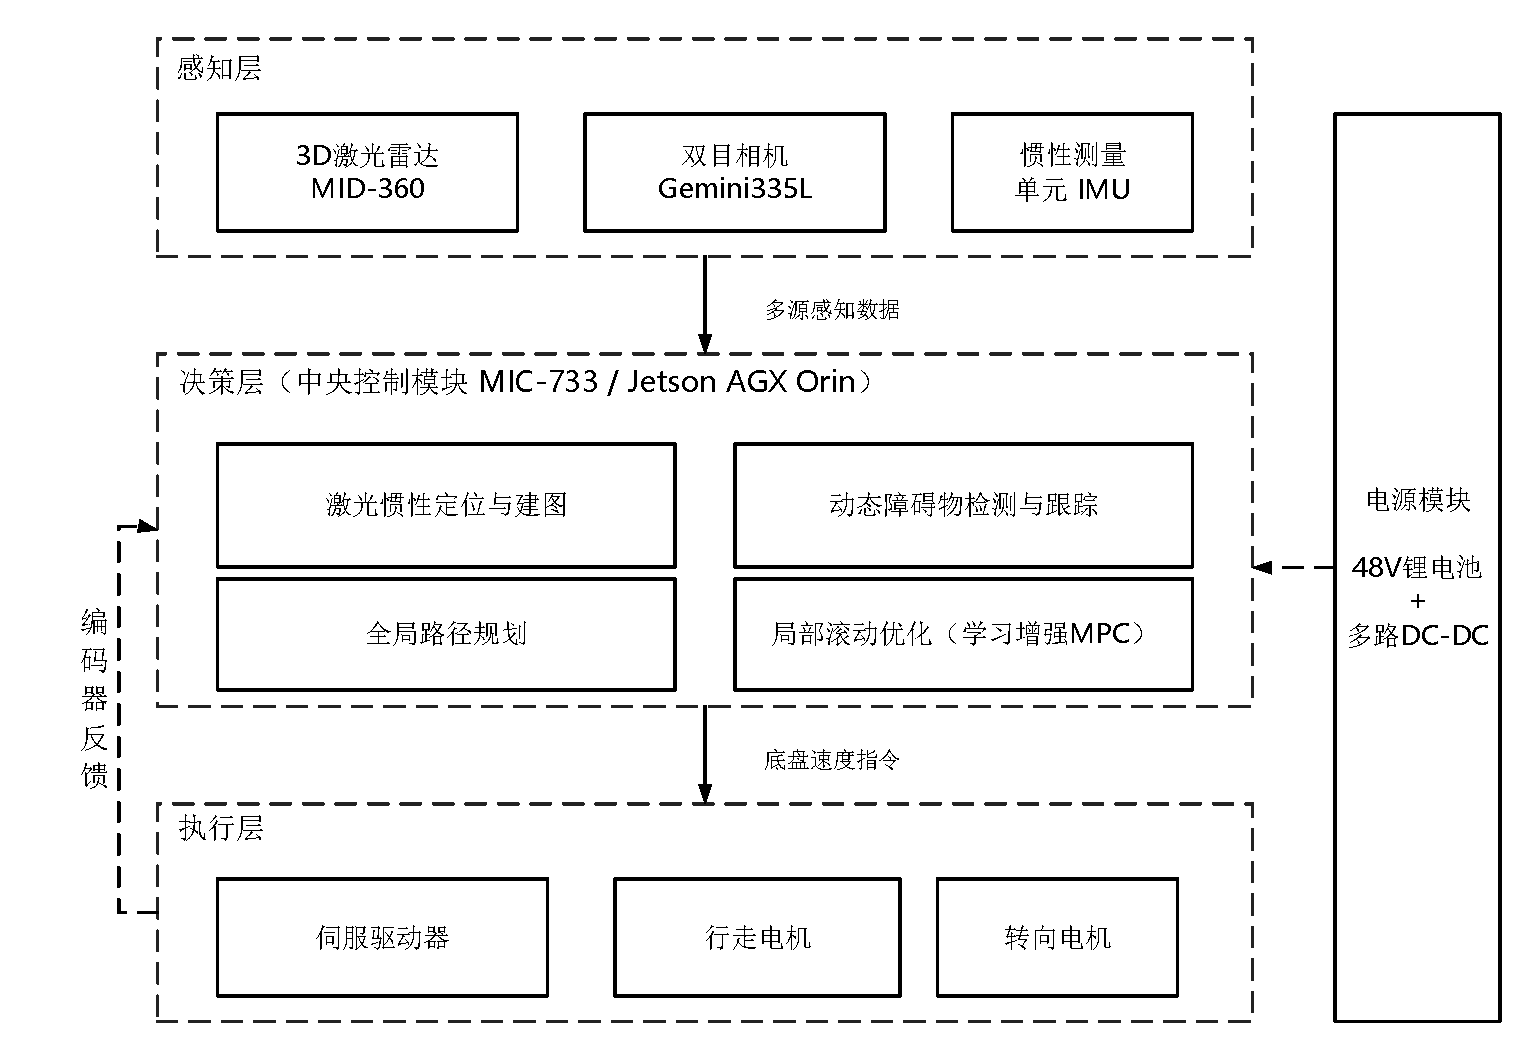
\includegraphics[width=0.95\textwidth]{pic/系统总体方案.pdf}
	\caption{机器人系统总体方案}
	\label{fig:系统总体方案}
\end{figure}

感知层位于系统底端，负责将物理环境转化为可计算的数字信息。该层由3D激光雷达、双目相机及雷达内置惯性测量单元（IMU）构成：激光雷达提供周围环境的三维点云，用于定位建图与障碍物几何提取；双目相机提供RGB图像与深度图像，用于工作目标识别与近场障碍感知；IMU提供高频角速度和加速度测量，为激光惯性里程计提供运动预测。各传感器以统一时间基准采集数据，经标准接口上传至中央控制模块。

决策层是系统的运算核心，由搭载高性能嵌入式计算平台的中央控制模块承担。该层订阅感知层上传的多源数据，依次完成激光惯性定位与地图构建、动态障碍物检测与跟踪、全局路径规划与局部滚动优化等任务，最终解算出满足运动学约束与避障要求的速度指令。考虑到激光点云配准、障碍物检测和模型预测控制等算法对算力的较高要求，决策层选用具备GPU并行加速能力的边缘计算平台，以保证导航算法的实时性。

执行层位于系统顶端，负责将决策层输出的速度指令转化为机器人的实际运动。该层由伺服驱动器、驱动电机和转向电机组成，通过CAN总线接收速度或位姿指令，驱动底盘按期望线速度和角速度运动，并将编码器反馈的实时转速、转角回传至中央控制模块，形成闭环控制。电源模块为上述各层提供稳定的多路供电，是系统持续可靠运行的能量基础。

上述分层方案使各模块职责清晰、接口规范，便于功能扩展与故障定位。下文将分别从硬件平台架构和软件系统架构两方面，对该方案的具体实现进行详细说明。

\section{机器人硬件平台架构}
\subsection{硬件选型}
机器人硬件结构包括传感器模块、中央控制模块、底层运动控制模块以及移动电源。传感器模块负责采集环境信息发送给中央控制器;
中央控制器处理传感器数据，计算出机器人运动控制指令并发送给底层运动控制模块；底层电机和舵机接受控制指令驱动机器人一定速度运动或变换到指定位姿。

\subsubsection{传感器模块}
传感器模块包括两部分：激光雷达和双目摄像头。3D激光雷达选用大疆览沃的MID-360，该激光雷达是4线束非重复扫描固态激光雷达，
由于体积小、重量轻、视场较大、分辨率较高，因此被广泛部署使用在机器人、割草机、无人车、工业和教育等智能产品中。
内部集成了IMU芯片（3轴加速度计和3轴陀螺仪），可结合点云数据构建高精地图并实现自主定位过程中的雷达坐标系、机器人坐标系、世界坐标系三者之间的转换关系。
激光雷达具体尺寸图如图~\ref{fig:Mid-360具体尺寸}所示，其性能参数如表~\ref{tab:mid360_params_centered}所示。

\begin{figure}[!htb]
	\centering
	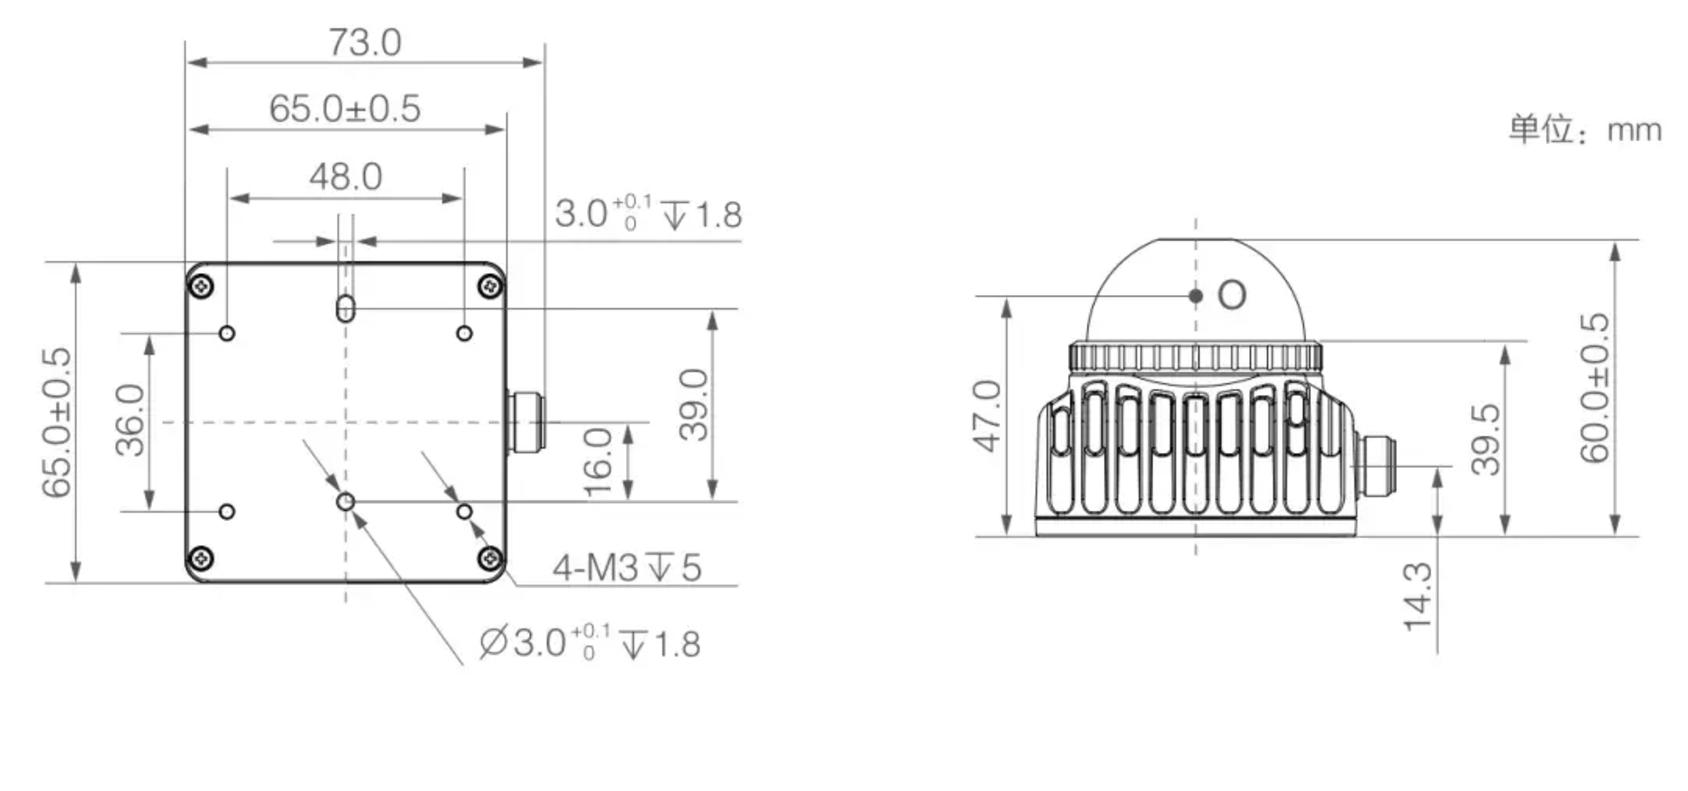
\includegraphics[width=\textwidth]{pic/激光雷达具体尺寸.pdf}
	\caption{激光雷达具体尺寸}
	\label{fig:Mid-360具体尺寸}
\end{figure}


\begin{table}[htbp]
  \centering
  \caption{MID360激光雷达性能参数}
  \label{tab:mid360_params_centered}
  \renewcommand{\arraystretch}{1.5} % 增大行间距
  \begin{tabularx}{\textwidth}{>{\centering\arraybackslash}X c c c c >{\centering\arraybackslash}X}
      \toprule[1.2pt]
      \textbf{项目} & \textbf{最小值} & \textbf{典型值} & \textbf{最大值} & \textbf{单位} & \textbf{备注} \\
      \midrule
      测距范围 & 0.1 & 10 & 40 & m & 100klux照度 \\
      测距精度 & - & ±5 & - & cm & 90\%反射率 \\
      水平视场角 & - & 360 & - & ° & 全向扫描 \\
      垂直视场角 & -7.0 & - & 52.0 & ° & - \\
      扫描模式 & - & 非重复扫描 & - & - & - \\
      虚警率 & - & <0.01\% & - & - & 100klux照度 \\
      工作温度 & -20 & - & 55 & °C & - \\
      工作电压 & 9 & - & 27 & V DC & - \\
      功耗 & - & 11 & - & W & 典型功耗 \\
      网络接口 & - & 千兆以太网 & - & - & 支持PTP、PPS \\
      \bottomrule[1.2pt]
  \end{tabularx}
\end{table}

图像采集模块包含两个双目摄像头，选用奥比中光公司的Gemini335L型号的摄像头，输出深度图像和RGB图像。
可用于目标检测、距离检测以及3D环境构建，本课题中双目摄像头主要用于移动机器人移动过程中对工作目标的识别。
双目摄像头参数见表~\ref{tab:gemini335l_params_adjusted}所示。
\begin{table}[h]
  \centering
  \caption{双目摄像头 Gemini335L 性能参数} 
  \label{tab:gemini335l_params_adjusted}
  \renewcommand{\arraystretch}{1.5} % 增大行间距
  \begin{tabularx}{\textwidth}{>{\centering\arraybackslash}X >{\centering\arraybackslash}X}
      \toprule[1.2pt] % 加粗顶线
      \textbf{规格参数} & \textbf{数值} \\
      \midrule
      最大工作范围 & 0.17-20m \\
      推荐工作范围 & 0.25-6m   \\
      基线        & 95mm         \\
      视场角      & 90°×65° @ 2m（1280×800）      \\
      分辨率      & 1280×800 @ 60fps         \\
      供电建议    & DC 5V \& $\geq$1.5A \\
      平均功耗    & < 3W \\
      工作温度    & -10-50°C \\
      \bottomrule[1.2pt] % 加粗底线
  \end{tabularx}
\end{table}

\subsubsection{中央控制模块}
中央控制模块是机器人系统的运算核心，需在有限的体积和功耗下同时承担激光惯性定位、点云处理、障碍物检测跟踪以及模型预测控制等计算密集型任务。综合考虑算力、接口丰富度、工业级可靠性和嵌入式部署要求，本文选用研华（Advantech）公司的MIC-733边缘AI推理计算机作为中央控制模块。该计算机以NVIDIA Jetson AGX Orin微型计算机为核心，集成Arm架构CPU与Ampere架构GPU，具备强大的并行计算与深度学习推理能力，可满足点云配准和滚动优化的实时性需求。同时，其工业级设计支持宽温、宽压工作，适应变电站等复杂工业环境。MIC-733的主要性能参数如表~\ref{tab:mic733_params}所示。

\begin{table}[htbp]
  \centering
  \caption{MIC-733中央控制器主要性能参数}
  \label{tab:mic733_params}
  \renewcommand{\arraystretch}{1.5}
  \begin{tabularx}{\textwidth}{>{\centering\arraybackslash}X >{\centering\arraybackslash}X}
      \toprule[1.2pt]
      \textbf{规格参数} & \textbf{数值} \\
      \midrule
      核心模块      & NVIDIA Jetson AGX Orin \\
      内存          & 32GB / 64GB LPDDR5 \\
      存储          & 64GB eMMC 5.1，支持M.2 2280 NVMe扩展 \\
      网络接口      & 4 $\times$ 10/100/1000 Mbps 千兆以太网 \\
      USB接口       & 2 $\times$ USB 2.0，4 $\times$ USB 3.2 Gen 2 \\
      串口          & 2 $\times$ RS-232/RS-422/RS-485 \\
      扩展接口      & 2 $\times$ Mini PCIe，1 $\times$ iDoor \\
      供电类型      & AT/ATX，DC 9$\sim$36V \\
      工作温度      & 0 $\sim$ +60°C \\
      尺寸 / 重量   & 192 $\times$ 230 $\times$ 87 mm / 4.5 kg \\
      \bottomrule[1.2pt]
  \end{tabularx}
\end{table}

MIC-733提供4个千兆以太网口，其中一个用于连接MID-360激光雷达并支持PTP时间同步，保证点云与IMU数据的时间一致性；USB 3.2接口用于连接双目相机，传输RGB与深度图像。由于底层伺服驱动器采用CAN总线通信，而Jetson平台默认不提供工业级CAN接口，本文通过其Mini PCIe扩展槽加装研华PCM-26D2CA双口隔离CAN扩展卡，该卡提供2路隔离CAN总线接口（DB9接插件），支持总线终端电阻跳线配置，从而实现中央控制模块与伺服驱动器之间的可靠通信。

\subsubsection{底层运动控制模块}
底层运动控制模块负责将中央控制模块输出的速度指令转化为底盘的实际运动。为满足运维机器人在变电站狭窄通道、设备密集区域灵活移动以及负载搬运的需求，底盘采用全向移动方案，选用凤凰动力（Phoenix Power）公司的PH210DS-A3-008-15卧式舵轮作为驱动与转向一体化执行单元。该舵轮将行走电机与转向电机集成于同一模块，行走部分负责提供前进驱动力，转向部分负责调整轮系朝向，二者协同实现底盘的全向运动。舵轮的主要参数如表~\ref{tab:steering_wheel_params}所示。

\begin{table}[htbp]
  \centering
  \caption{PH210DS卧式舵轮主要参数}
  \label{tab:steering_wheel_params}
  \renewcommand{\arraystretch}{1.4}
  \begin{tabularx}{\textwidth}{>{\centering\arraybackslash}X c c >{\centering\arraybackslash}X}
      \toprule[1.2pt]
      \textbf{部件} & \textbf{参数} & \textbf{数值} & \textbf{单位} \\
      \midrule
      \multirow{6}{*}{行走部分} & 额定电压 & 48 & V DC \\
                               & 额定功率 & 1100 & W \\
                               & 额定扭矩 / 峰值扭矩 & 4.2 / 12.6 & N$\cdot$m \\
                               & 额定转速 / 额定电流 & 2500 / 25 & rpm / A \\
                               & 驱动轮径 / 速比 & 210 / 24.685 & mm / -- \\
                               & 编码器 & 增量式 2500ppr & -- \\
      \midrule
      \multirow{5}{*}{转向部分} & 额定电压 & 48 & V DC \\
                               & 额定功率 & 400 & W \\
                               & 额定扭矩 / 峰值扭矩 & 1.27 / 3.81 & N$\cdot$m \\
                               & 最大转向速度 & 81.82 & °/s \\
                               & 编码器 & 17bit 绝对值 & -- \\
      \midrule
      \multirow{4}{*}{整机}    & 驱动轮载荷 & 800 & kg \\
                               & 机械限位 / 电子限位 & $\pm$135 / $\pm$125 & ° \\
                               & 制动器电压 / 扭矩 & 24 / 6 & V DC / N$\cdot$m \\
                               & 防护等级 & IP65 & -- \\
      \bottomrule[1.2pt]
  \end{tabularx}
\end{table}

舵轮的行走电机与转向电机均为交流伺服电机，需配套伺服驱动器进行闭环控制。行走电机额定功率1100W、额定电流25A，转向电机额定功率400W、额定电流10A，二者功率与电流等级差异较大。为此，本文针对不同电机分别选配伺服驱动器：行走电机选用凤凰动力PLD2L-CAN系列驱动器，转向电机选用步科（Kinco）FD1X5系列驱动器。两类驱动器均支持CANopen（CiA DSP402）总线协议，可与中央控制模块的CAN扩展卡组网通信，并支持位置、速度、转矩多种控制模式。两款伺服驱动器的主要参数对比如表~\ref{tab:servo_driver_params}所示。

\begin{table}[htbp]
  \centering
  \caption{伺服驱动器主要参数对比}
  \label{tab:servo_driver_params}
  \renewcommand{\arraystretch}{1.4}
  \begin{tabularx}{\textwidth}{>{\centering\arraybackslash}X >{\centering\arraybackslash}X >{\centering\arraybackslash}X}
      \toprule[1.2pt]
      \textbf{参数} & \textbf{凤凰 PLD2L-CAN} & \textbf{步科 FD1X5} \\
      \midrule
      适配电机      & 行走电机（1100W）     & 转向电机（400W） \\
      主电源电压    & 24 $\sim$ 70V DC      & 24 $\sim$ 60V DC \\
      额定输出电流  & 5 $\sim$ 30 Arms（分档） & 15 / 30 / 50 Arms（分档） \\
      控制方式      & SVPWM正弦波控制       & 矢量控制 \\
      总线协议      & CANopen (DSP402)      & CAN / Modbus / EtherCAT \\
      控制模式      & 位置 / 速度 / 转矩    & 位置 / 速度 / 转矩 \\
      反馈信号      & 多摩川协议编码器      & 多摩川协议编码器 \\
      抱闸输出      & 支持（直接驱动）      & 支持（24V直接驱动） \\
      \bottomrule[1.2pt]
  \end{tabularx}
\end{table}

工作时，中央控制模块将解算得到的底盘速度指令分解为各舵轮的行走速度和转向角度，经CAN总线下发至对应伺服驱动器；驱动器驱动电机运动，并将编码器测得的实时转速、转角通过CAN总线回传，实现速度与位置的闭环控制。转向部分采用17bit绝对值编码器，可在上电时直接获取绝对转角，无需回零操作，提高了系统启动效率与定位精度。

\subsubsection{电源模块}
电源模块为机器人各功能单元提供稳定可靠的电能。系统内不同部件的供电需求各异：舵轮行走与转向电机需48V直流供电，制动器与驱动器逻辑电路需24V直流供电，中央控制模块支持9$\sim$36V宽压输入，激光雷达需9$\sim$27V直流供电，双目相机需5V直流供电。为统一管理上述多路供电，本文采用以48V锂电池组为主电源、配合多路DC-DC变换的供电架构：48V母线直接为舵轮电机供电，并经DC-DC降压模块分别转换为24V、12V和5V，为驱动器逻辑、工控机、激光雷达和相机等部件供电。各供电支路独立布线并设置过流、过压保护，避免电机启停时的电流冲击影响控制与感知系统的稳定运行。

\subsection{硬件结构连接}
在完成各功能模块选型的基础上，本节阐述机器人硬件各部件之间的物理连接与信号交互关系，整体硬件连接拓扑如图~\ref{fig:硬件连接拓扑}所示。系统以MIC-733中央控制模块为核心，向上通过标准数据接口连接感知设备，向下通过CAN总线连接执行设备，形成”传感器--控制器--驱动器--电机”的完整信号链路。

\begin{figure}[!htb]
	\centering
	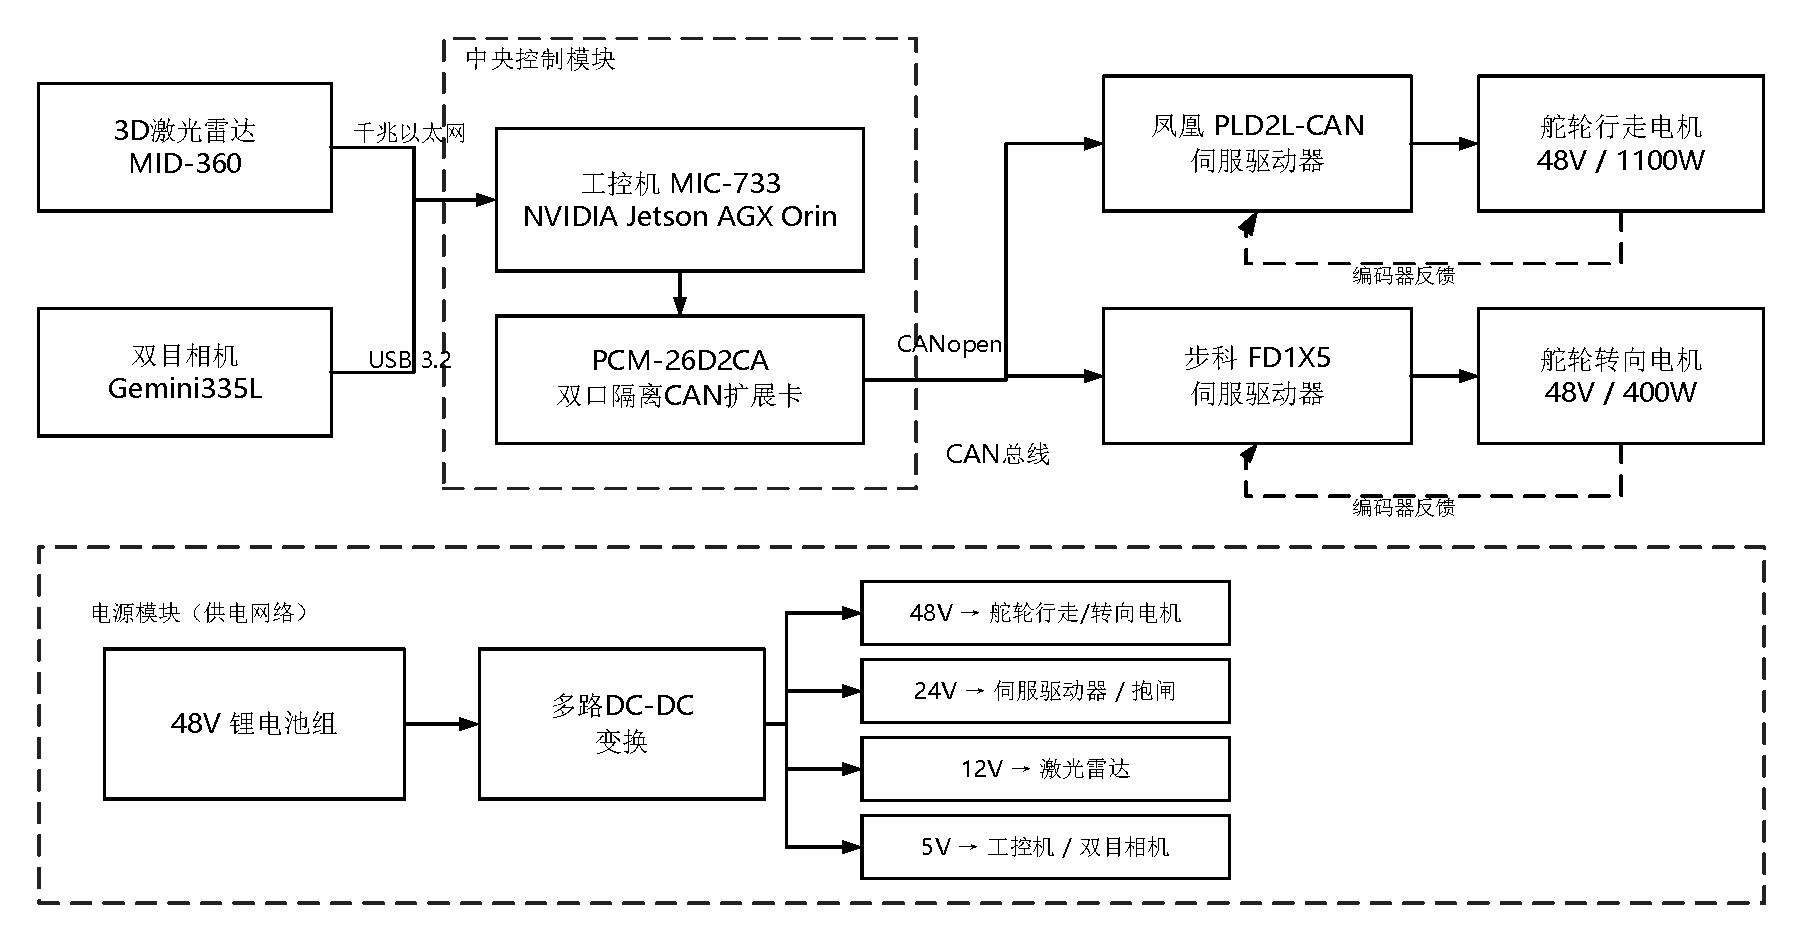
\includegraphics[width=\textwidth]{pic/硬件连接拓扑.pdf}
	\caption{机器人硬件连接拓扑}
	\label{fig:硬件连接拓扑}
\end{figure}

在感知数据链路上，MID-360激光雷达通过千兆以太网接入MIC-733的LAN口，利用PTP/PPS实现与系统时钟的硬件同步；双目相机通过USB 3.2接口连接工控机，传输RGB与深度图像数据。在控制指令链路上，工控机经Mini PCIe扩展的PCM-26D2CA双口CAN卡引出两路隔离CAN总线，分别连接行走电机驱动器（凤凰PLD2L-CAN）和转向电机驱动器（步科FD1X5）。CAN总线采用主从结构，工控机作为主站周期性下发速度与位置指令，驱动器作为从站执行指令并反馈电机状态，总线终端按规范配置120\,$\Omega$终端电阻以保证通信质量。在能量供给链路上，48V锂电池组经配电单元和DC-DC变换为各部件分配相应电压等级的电源。通过上述连接方式，各模块在统一的硬件框架下协同工作，为软件系统的运行提供物理基础。

\section{机器人软件系统架构}
机器人软件系统基于机器人操作系统（Robot Operating System, ROS）构建，运行于Ubuntu 20.04操作系统与ROS Noetic发行版之上。ROS采用分布式节点架构，各功能模块以独立节点（Node）形式运行，节点之间通过话题（Topic）、服务（Service）和动作（Action）等机制进行消息通信，并借助参数服务器和坐标变换（TF）工具统一管理系统参数与多坐标系关系。这种松耦合的设计使感知、定位、规划和控制等模块能够独立开发、测试与替换，便于系统的迭代与维护。机器人软件系统总体架构如图~\ref{fig:软件系统架构}所示，自下而上可划分为传感器驱动层、感知与定位层、规划决策层和运动控制层四个层次。

\begin{figure}[!htb]
	\centering
	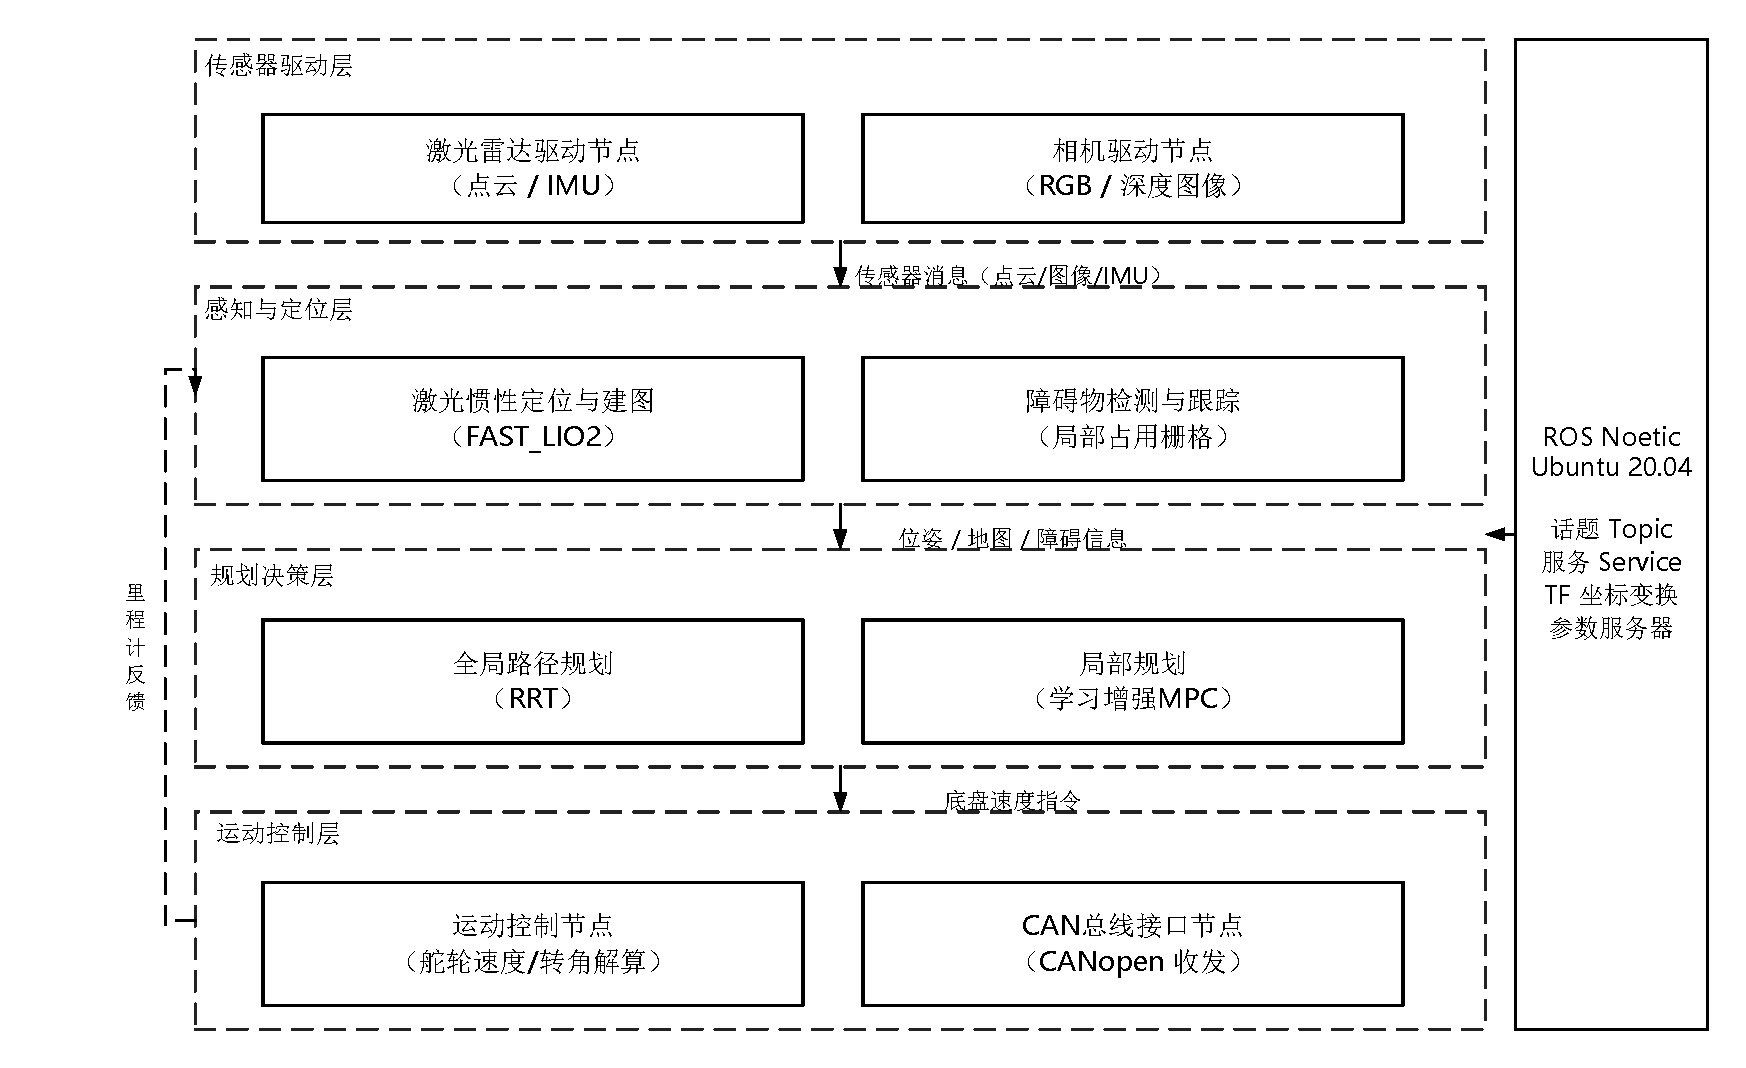
\includegraphics[width=0.92\textwidth]{pic/软件系统架构.pdf}
	\caption{机器人软件系统架构}
	\label{fig:软件系统架构}
\end{figure}

传感器驱动层负责采集并发布原始传感器数据。激光雷达驱动节点发布三维点云与IMU数据，相机驱动节点发布RGB图像与深度图像，各驱动节点将数据封装为标准ROS消息（如\texttt{sensor\_msgs/PointCloud2}、\texttt{sensor\_msgs/Image}、\texttt{sensor\_msgs/Imu}）并以话题形式向上层发布，为后续处理提供统一的数据输入。

感知与定位层是环境理解的核心。该层包含激光惯性定位建图节点和障碍物检测跟踪节点：前者基于FAST\_LIO2算法融合点云与IMU数据，在预建地图坐标系下输出机器人的全局位姿与里程计信息；后者融合深度图像与点云数据，检测并跟踪环境中的静态与动态障碍物，输出障碍物包围盒与状态估计结果，同时维护局部占用栅格地图。该层输出的位姿、地图和障碍信息为规划决策提供环境约束。

规划决策层根据导航任务和环境信息生成运动轨迹。全局规划节点基于预建地图和目标点，采用RRT算法生成全局参考路径；局部规划节点以全局路径为参考，融合实时障碍信息，通过学习增强MPC在滚动时域内求解满足运动学约束、平滑约束和避障要求的局部轨迹，并输出底盘速度指令。

运动控制层负责将速度指令转化为电机执行动作。运动控制节点将规划层输出的底盘速度指令分解为各舵轮的行走速度与转向角度，通过CAN总线接口节点按CANopen协议下发至伺服驱动器，并接收编码器反馈，实现底盘运动的闭环控制。

上述四层结构与硬件平台一一对应，数据自下而上逐层抽象、指令自上而下逐层细化，共同构成功能完整、层次清晰的机器人导航软件系统。

\section{本章小结}
本章面向变电站运维机器人的应用需求，完成了机器人系统框架的总体设计。首先，结合变电站高安全性、高可靠性和复杂空间约束的特点，分析了机器人在环境感知、定位建图、自主导航和动态避障四个方面的功能需求。其次，提出了”感知--决策--执行”的分层模块化系统方案，明确了传感器模块、中央控制模块、底层运动控制模块和电源模块的职责划分与协作关系。在此基础上，完成了硬件平台选型：感知模块选用MID-360激光雷达和Gemini335L双目相机，中央控制模块选用基于NVIDIA Jetson AGX Orin的研华MIC-733计算机并扩展CAN接口，底层运动控制模块选用凤凰动力PH210DS卧式舵轮，并分别为行走电机和转向电机配套凤凰PLD2L-CAN和步科FD1X5伺服驱动器，电源模块采用48V锂电池配合多路DC-DC变换的供电架构。随后，阐述了各部件之间的硬件连接拓扑与信号交互关系。最后，基于ROS设计了由传感器驱动层、感知与定位层、规划决策层和运动控制层构成的软件系统架构。本章设计的软硬件框架为后续各章的定位、感知与路径规划算法研究提供了统一的实现平台。




\chapter{基于FAST-LIO2的激光里程计定位算法研究}
\section{引言}
稳定可靠的自身定位是移动机器人在复杂动态环境中完成运输、巡检、侦察和辅助作业的前提。机器人只有在统一坐标系下持续获得准确的全局位姿，才能为后续的环境感知、障碍物检测与路径规划提供可信的空间基准。厂房、仓储空间、地下通道和大型设施内部往往结构重复、纹理单一且GNSS信号受限，单纯依靠轮式里程计或二维激光定位难以长期维持精度，容易产生累积漂移并在退化区域失效。因此，需要一种能够融合多源信息、在已知环境中提供稳定绝对定位的方法。

实时定位与地图构建（Simultaneous Localization and Mapping，SLAM）是移动机器人与自动驾驶领域的核心技术。其核心任务可归结为一种耦合估计问题：在未知环境中，移动平台利用传感器数据，同步完成对自身运动状态的描述与对环境空间结构的建模。二者相互依赖，定位精度依赖于地图的准确性，而一致地图的构建又需以精确的位姿轨迹为前提。在众多SLAM方案中，紧耦合激光惯性里程计因其高精度、低延迟和对退化环境的鲁棒性，逐渐成为三维定位的主流选择，其中FAST-LIO2以直接点到地图配准和迭代卡尔曼滤波取得了良好的精度与实时性平衡。

然而，原始FAST-LIO2更侧重在线里程计与建图，其输出轨迹仍可能随运行距离产生累积漂移，难以直接满足已知场景重复作业对可复现绝对位姿的需求。针对这一问题，本章在FAST-LIO2直接激光惯性里程计框架基础上，引入预建点云地图约束与有初值重定位机制，将在线里程计问题转化为地图坐标系下的连续位姿估计问题，并从定位精度、初始对齐鲁棒性和计算开销三个方面对所述方法进行仿真验证。

本章的主要内容如下：

（1）系统阐述SLAM的基本架构与技术分类，并重点剖析FAST-LIO2的核心原理，包括IMU状态传播、激光点云运动畸变补偿、直接点到地图残差、流形迭代卡尔曼滤波以及ikd-Tree增量地图维护机制。

（2）提出面向预建PCD地图的定位与启动重定位方法。通过加载预建地图构建空间索引，采用“近似初值 + ICP精配准”的两阶段策略完成地图坐标系下的初始对齐，并在滤波器量测更新阶段利用固定全局地图提供几何先验，抑制纯里程计运行中的坐标漂移。

（3）区分纯定位模式与混合建图模式，使所述方法能够在固定地图重复作业与地图扩展两类任务之间灵活切换，为不同工业与特种作业场景提供统一的状态估计框架。

（4）在Gazebo仿真环境中设置走廊、迷宫和圆柱体林三类场景，对比纯定位、混合建图与纯里程计三种模式的绝对轨迹误差和相对位姿误差，评估初始对齐在不同初值扰动下的收敛性能，并统计各模块计算耗时以验证算法的实时性。

\section{SLAM方法架构及技术分类}
同步定位与地图构建是一个由前端里程计、后端优化、回环检测和地图维护等模块共同完成的状态估计问题。前端对相邻时刻的传感器观测进行关联与配准，实时估计平台的增量运动并形成局部一致的轨迹；回环检测在机器人重访历史区域时提供非连续时刻之间的约束；后端将里程计约束与回环约束组织为概率估计问题，以减小累积漂移；建图模块则依据估计轨迹将传感器观测融合至统一坐标系。按主要传感器可分为激光雷达SLAM、视觉SLAM和多传感器融合SLAM；按估计框架可分为基于滤波器的方法与基于图优化的方法。

\subsection{基于滤波器的SLAM}
基于滤波器的SLAM方法将系统的状态（包括机器人位姿与环境路标点）建模为一个随时间演进的概率分布。
其核心思想是采用递归的贝叶斯估计框架，在每一时刻，根据当前的控制输入和传感器观测，对系统状态的置信度（后验概率）进行更新。
最具代表性的方法是扩展卡尔曼滤波器（EKF-SLAM）及其改进算法。EKF-SLAM通过线性化非线性运动与观测模型，在状态向量的高斯分布假设下，进行均值和协方差的递推更新。
此类方法的优势在于能够提供状态的在线估计及其不确定性度量，且计算复杂度与路标数量相关。然而，其线性化误差可能导致滤波器发散，且通常假设数据关联是已知或准确的。
FastSLAM算法通过粒子滤波估计路径，结合EKF估计路标，部分克服了EKF-SLAM的局限性，但粒子退化问题依然存在。在计算资源受限、强调实时性的应用场景中，基于滤波器的轻量化变体（如迭代卡尔曼滤波）仍具有重要价值。

\subsection{基于图优化的SLAM}
基于图优化的SLAM是当前主流的高精度SLAM框架。该方法将SLAM问题转化为一个大规模非线性最小二乘优化问题。其模型是一个图结构：节点表示机器人不同时刻的位姿（有时也包括环境路标），边则表示位姿节点之间的空间约束。
边主要分为两种：一是由前端里程计产生的连续位姿间的约束（里程计边），二是由回环检测产生的非连续位姿间的约束（回环边）。当检测到回环时，相当于在图中添加了新的强约束，
从而能够有效校正累积的里程计漂移。优化目标是寻找一组最优的节点状态（位姿），使得图中所有边代表的预测观测与实际观测之间的误差平方和最小。常用的优化工具包括高斯-牛顿法、列文伯格-马夸尔特算法等。
与滤波器方法相比，图优化方法能更自然地融合回环约束，进行全局一致性优化，从而获得精度更高的轨迹和地图，但其通常作为后端批量或滑动窗口优化运行，对计算资源要求较高。g2o、GTSAM、Ceres Solver等开源库为图优化SLAM的实现提供了强大支撑。

\subsection{紧耦合激光-惯性SLAM}
紧耦合激光-惯性SLAM是当前实现高鲁棒性、高频率状态估计的主流方案，其核心在于对激光雷达与惯性测量单元（IMU）的数据进行深层次融合。IMU能够以数百赫兹的频率测量角速度和加速度，在短时间内积分可提供高频但快速发散的位姿预测。
激光雷达则提供低频但绝对精度较高的三维几何观测。紧耦合方法并非将二者独立处理后再进行结果融合，而是在一个统一的状态估计框架内，直接使用原始的激光雷达点云和IMU测量值，共同约束系统状态（通常包括位置、姿态、速度、传感器偏置等）。
具体而言，激光雷达的每一个或多个原始点都可以直接作为观测方程，与IMU预测的运动方程一起，构建一个状态估计问题。这种深度融合方式充分利用了IMU的高频动态信息来辅助激光雷达点云的运动畸变矫正和数据关联，同时利用激光雷达的精确观测来抑制IMU积分漂移。
以FAST-LIO系列为代表的算法，通过将紧耦合的激光-惯性里程计建模在迭代卡尔曼滤波框架下，实现了在剧烈运动场景中的鲁棒、实时、高精度状态估计，是紧耦合SLAM的典型代表\textsuperscript{\cite{Xu2021FASTLIO}}。

\section{FAST-LIO2激光惯性里程计原理}
FAST-LIO2是一类面向实时三维建图与定位的紧耦合激光惯性里程计方法，其核心思想是在误差状态迭代卡尔曼滤波框架内融合IMU传播模型与激光点云到局部地图的几何约束\textsuperscript{\cite{Xu2022FASTLIO2}}。与LOAM类方法先提取边缘点、平面点再进行特征匹配的流程不同\textsuperscript{\cite{Zhang2014LOAM}}，FAST-LIO2取消了手工特征提取模块，直接使用降采样后的原始激光点与地图进行配准。这种直接法能够保留更多环境几何信息，降低算法对雷达扫描模式和特征阈值的依赖，因此更适合Livox MID360等非重复扫描或小型移动平台常用的三维激光雷达。

FAST-LIO2的系统流程可概括为：首先，利用IMU高频测量对状态进行前向传播，并在传播过程中对一帧激光点云内部的运动畸变进行补偿；其次，将去畸变后的点云变换到世界坐标系，在增量地图中搜索近邻点并拟合局部平面；最后，根据点到局部平面的残差构造量测模型，通过迭代卡尔曼滤波更新位姿、速度、IMU偏置以及外参等状态。为保证实时性，FAST-LIO2采用增量式$k$维树（ikd-Tree）维护点云地图，使地图能够在线支持点插入、删除、重平衡和近邻搜索，避免每一帧重新构建静态KD树带来的高计算开销\textsuperscript{\cite{Cai2021ikdTree}}。

\begin{figure}[htbp]
  \centering
  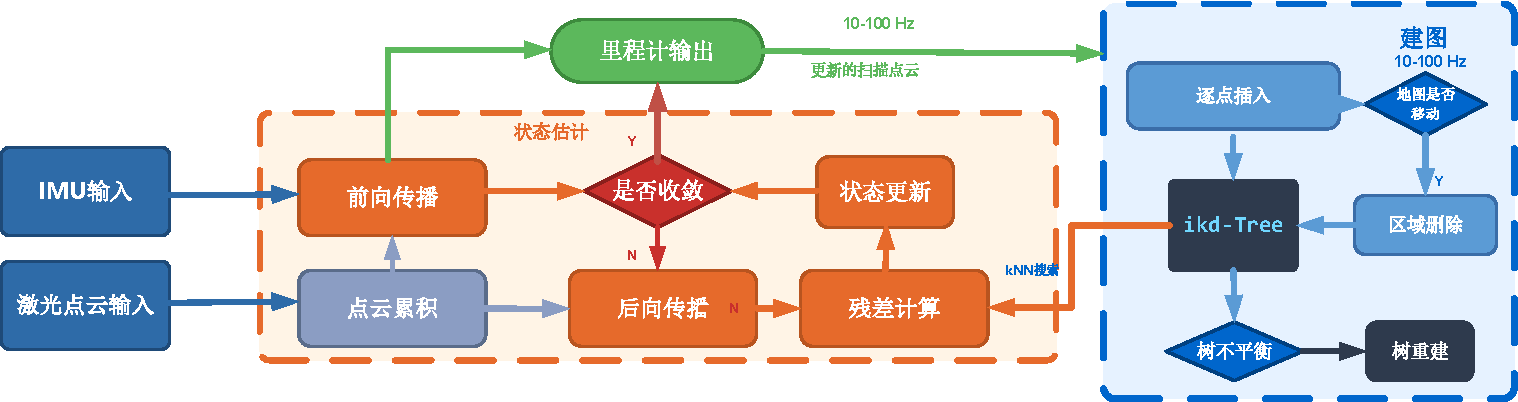
\includegraphics[width=\linewidth]{pic/激光惯性里程计系统架构.pdf}
  \caption{FAST-LIO2激光惯性里程计系统架构}
  \label{fig:fastlio_arch}
\end{figure}

FAST-LIO2由状态估计与增量地图维护两部分构成。状态估计模块采用迭代误差状态卡尔曼滤波（Iterated Error-State Kalman Filter, IESKF），依次完成IMU前向传播、点云运动畸变补偿、点到局部平面残差构造和迭代量测更新，输出高频位姿估计；地图维护模块采用增量式$k$维树（ikd-Tree）执行近邻搜索、树上降采样、增量插入、区域删除与动态重平衡。状态估计结果既作为导航系统的位姿反馈，也用于将当前点云变换至地图坐标系并更新空间索引。

\subsection{状态变量与IMU传播模型}
图~\ref{fig:fastlio_arch}展示了FAST-LIO2的系统流程。每组同步数据到达后，系统首先利用IMU测量传播状态，并按点的相对时间戳补偿一帧点云内部的运动畸变；随后将去畸变点云变换至世界坐标系，在ikd-Tree地图中搜索近邻并拟合局部平面；最后在当前线性化点处构造点到平面残差与雅可比，通过迭代量测更新修正状态。若状态增量满足收敛阈值，则输出当前位姿；否则在新的线性化点重新构造量测并继续迭代，直至收敛或达到最大迭代次数。地图维护模块根据当前位姿移动局部地图窗口，删除窗口外点云，并将具有新增几何信息的当前帧点增量插入ikd-Tree。

设系统状态定义为
\begin{equation}
    \mathbf{x}
    =
    \left[
    {}^{G}\mathbf{p}_{I}^{T},
    {}^{G}\mathbf{R}_{I},
    {}^{I}\mathbf{R}_{L},
    {}^{I}\mathbf{p}_{L}^{T},
    {}^{G}\mathbf{v}_{I}^{T},
    \mathbf{b}_{g}^{T},
    \mathbf{b}_{a}^{T},
    {}^{G}\mathbf{g}^{T}
    \right],
    \label{eq:fastlio_state}
\end{equation}
其中${}^{G}\mathbf{p}_{I}$、${}^{G}\mathbf{R}_{I}$分别表示IMU坐标系相对于全局坐标系的位置和姿态，${}^{I}\mathbf{R}_{L}$、${}^{I}\mathbf{p}_{L}$表示激光雷达相对于IMU的外参，${}^{G}\mathbf{v}_{I}$为IMU速度，$\mathbf{b}_{g}$、$\mathbf{b}_{a}$分别为陀螺仪和加速度计偏置，${}^{G}\mathbf{g}$为重力向量。上述状态同时包含运动状态、传感器误差项和外参项，使激光几何约束能够与惯性传播约束在同一估计框架内共同作用。

IMU测量可表示为
\begin{equation}
    \boldsymbol{\omega}_{m}=\boldsymbol{\omega}+\mathbf{b}_{g}+\mathbf{n}_{g},
    \quad
    \mathbf{a}_{m}=\mathbf{a}+\mathbf{b}_{a}+\mathbf{n}_{a},
    \label{eq:imu_measurement}
\end{equation}
其中$\boldsymbol{\omega}_{m}$和$\mathbf{a}_{m}$为IMU输出的角速度和加速度，$\mathbf{n}_{g}$、$\mathbf{n}_{a}$为测量噪声。连续时间状态传播可写为
\begin{equation}
\begin{aligned}
    {}^{G}\dot{\mathbf{p}}_{I} &= {}^{G}\mathbf{v}_{I},\\
    {}^{G}\dot{\mathbf{R}}_{I} &= {}^{G}\mathbf{R}_{I}
    \left(\boldsymbol{\omega}_{m}-\mathbf{b}_{g}-\mathbf{n}_{g}\right)^{\wedge},\\
    {}^{G}\dot{\mathbf{v}}_{I} &= {}^{G}\mathbf{R}_{I}
    \left(\mathbf{a}_{m}-\mathbf{b}_{a}-\mathbf{n}_{a}\right)
    +{}^{G}\mathbf{g},\\
    \dot{\mathbf{b}}_{g} &= \mathbf{n}_{bg},\quad
    \dot{\mathbf{b}}_{a} = \mathbf{n}_{ba}.
\end{aligned}
    \label{eq:imu_propagation}
\end{equation}
式中$(\cdot)^{\wedge}$表示李代数向量到反对称矩阵的映射。由于激光雷达在采集一帧点云时平台仍在连续运动，若直接将整帧点云视为同一时刻采集，会在快速转弯或加减速时产生明显运动畸变。FAST-LIO2利用IMU传播得到的连续位姿，对每个点按照其相对时间戳进行反向补偿，将其统一到该帧结束时刻，从而提升后续点云配准的一致性。

\subsection{直接点到地图量测模型}
在量测更新阶段，FAST-LIO2将去畸变后的激光点${}^{L}\mathbf{p}_{j}$根据当前状态变换到全局坐标系：
\begin{equation}
    {}^{G}\mathbf{p}_{j}
    =
    {}^{G}\mathbf{R}_{I}
    \left(
    {}^{I}\mathbf{R}_{L}{}^{L}\mathbf{p}_{j}
    +{}^{I}\mathbf{p}_{L}
    \right)
    +{}^{G}\mathbf{p}_{I}.
    \label{eq:point_transform}
\end{equation}
随后在ikd-Tree维护的地图中搜索该点的若干近邻点，并利用近邻点拟合局部平面
\begin{equation}
    \mathbf{u}_{j}^{T}\mathbf{p}+d_{j}=0,
    \label{eq:local_plane}
\end{equation}
其中$\mathbf{u}_{j}$为平面单位法向量，$d_{j}$为平面参数。对应的点到平面残差为
\begin{equation}
    r_{j}
    =
    \mathbf{u}_{j}^{T}{}^{G}\mathbf{p}_{j}
    +d_{j}.
    \label{eq:point_plane_residual}
\end{equation}
该残差直接反映当前状态估计下激光点与局部地图几何的一致性。实际量测构造过程包括坐标变换、近邻搜索、局部平面估计、残差筛选和量测雅可比计算等步骤。当有效点数量不足或近邻无法稳定拟合平面时，系统应降低该帧几何约束的可信度，以避免退化环境对滤波器造成错误修正。

设一帧中所有有效点残差堆叠为$\mathbf{r}$，量测模型可近似写为
\begin{equation}
    \mathbf{0}
    =
    \mathbf{h}(\mathbf{x})+\mathbf{v},
    \quad
    \mathbf{h}(\mathbf{x})=
    \left[r_{1},r_{2},\cdots,r_{m}\right]^{T},
    \label{eq:fastlio_measurement}
\end{equation}
其中$m$为有效量测点数量，$\mathbf{v}$为激光量测噪声。由于位姿状态位于$SO(3)$流形上，FAST-LIO2采用流形上的误差状态迭代卡尔曼滤波进行求解：先由IMU传播得到预测状态，再在当前线性化点附近反复构建点到平面残差和雅可比，迭代修正误差状态，直至收敛或达到最大迭代次数。与传统ICP单独输出刚体变换不同，该过程将点云几何约束直接融入包含IMU偏置、速度和外参的统一状态估计中，因此能够同时获得低延迟和较高鲁棒性。

\subsection{基于ikd-Tree的增量地图维护}
\label{subsec:ikdtree_maintenance}
激光里程计需要在每帧点云到来时进行地图近邻搜索和地图更新。若每次都对全局点云重新构建KD树，计算复杂度会随着地图规模迅速上升，难以满足在线定位需求。FAST-LIO2使用ikd-Tree维护局部稠密点云地图，该结构除支持近邻搜索外，还支持增量插入、按空间区域删除、树结构重平衡以及树上体素降采样。

如图~\ref{fig:fastlio_arch}右侧所示，ikd-Tree除提供$k$近邻搜索外，还需随机器人运动动态维护局部地图窗口。当机器人接近当前地图窗口边界时，系统平移局部窗口并删除窗口外的历史点，以限制内存与查询规模。插入新点前，ikd-Tree执行树上降采样（On-Tree Downsampling）：若对应体素内已有更具代表性的地图点，且新点不能提供额外几何约束，则跳过插入；否则将新点增量加入树结构。频繁插入与删除可能导致树结构失衡，当不平衡度超过阈值时，系统触发局部或全局重构，以恢复近邻查询效率。

本文采用的地图维护策略与FAST-LIO2一致：系统首先将当前帧降采样点云变换到世界坐标系，再依据体素分辨率判断新观测是否能够补充地图几何信息。若某一体素内已经存在更具代表性的地图点，则当前点不再重复插入；若当前点能够提供新的空间约束，则将其作为增量点加入地图索引。对于预建地图定位任务，地图更新可以被关闭，使所有量测始终约束在固定的全局地图中；对于未知区域探索或地图扩展任务，则可在完成初始定位后开启增量更新，使新观测逐步并入原有地图。该策略使定位模式和建图扩展模式能够在同一状态估计框架下统一描述。

\section{面向预建地图的FAST-LIO2定位与重定位方法}
\label{sec:prebuilt_map_localization}
原始FAST-LIO2更侧重在线里程计与建图，其输出轨迹不可避免地存在长距离累积漂移。对于移动机器人在已知厂房、仓储空间、地下通道或大型设施内部执行重复作业的任务，系统更需要在预先构建的全局点云地图中获得稳定、可复现的绝对位姿。因此，本文在FAST-LIO2直接激光惯性里程计框架基础上，引入预建点云地图约束和有初值重定位机制，将在线里程计问题转化为地图坐标系下的连续位姿估计问题。该方法并非改变FAST-LIO2的紧耦合状态估计本质，而是在滤波器量测更新阶段使用固定全局地图提供几何先验，从而抑制纯里程计运行中的坐标漂移。

本文所提出的定位框架如图~\ref{fig:map_localization}所示，系统分为初始化（阶段A）和在线定位（阶段B）两个阶段。阶段A完成地图加载与ikd-Tree索引构建、IMU静态初始化以及近似初值与ICP相结合的两阶段初始对齐，为后续状态估计提供可靠的初始位姿；阶段B在每帧数据到来时执行IMU传播、点云去畸变、地图坐标变换、ikd-Tree近邻搜索与IEKF状态更新，持续输出地图坐标系下的全局连续位姿，并可根据任务需求在纯定位模式与混合建图模式之间切换。

\begin{figure}[htbp]
  \centering
  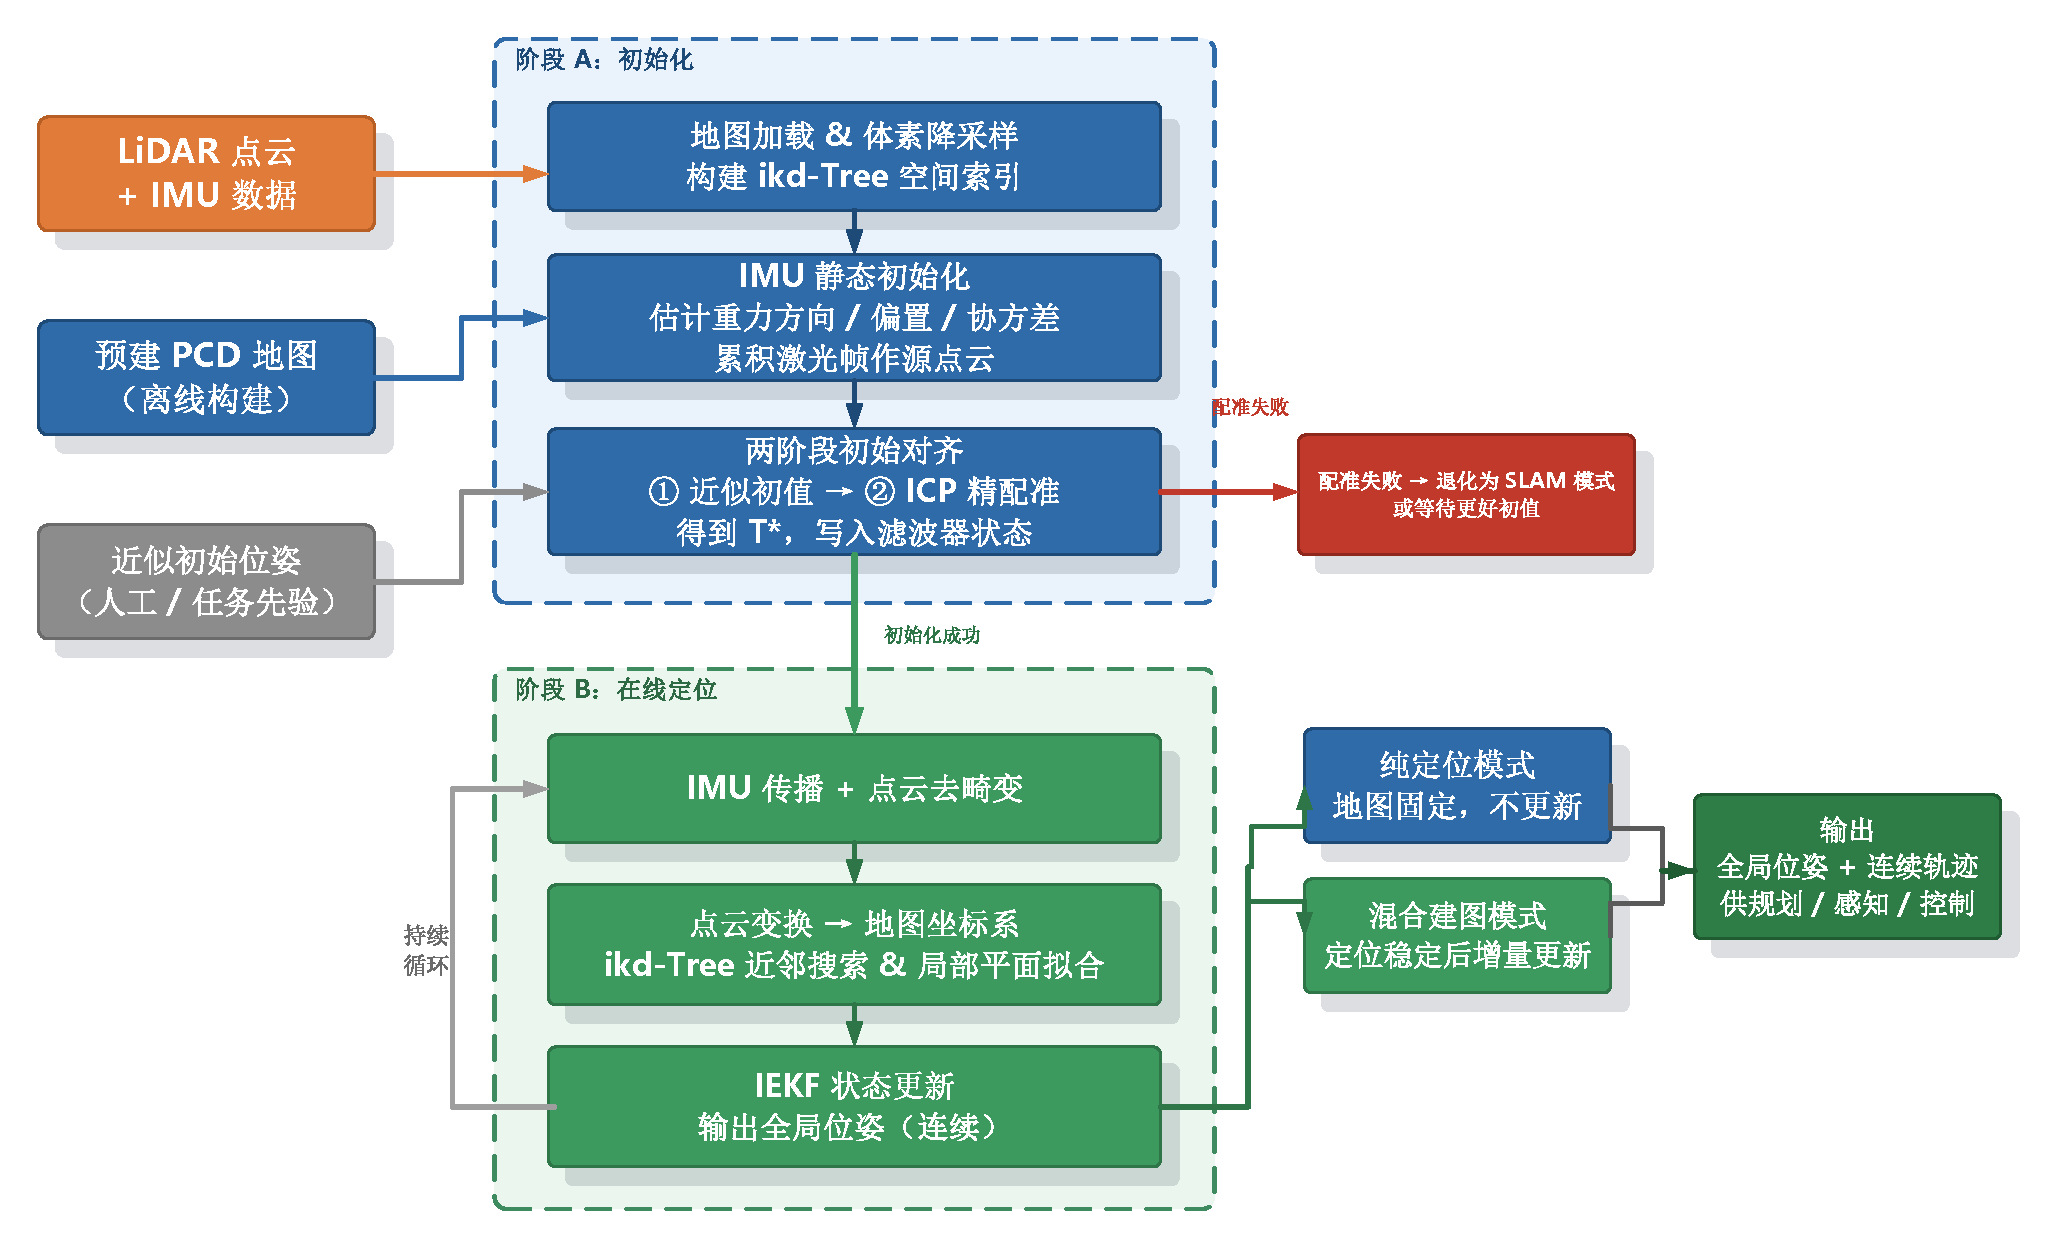
\includegraphics[width=0.92\linewidth]{pic/预建地图定位框架.pdf}
  \caption{基于预建地图的FAST-LIO2定位框架}
  \label{fig:map_localization}
\end{figure}

\subsection{预建地图定位框架}
预建地图定位系统的输入由三部分构成：一是连续到达的激光雷达点云和IMU测量，二是离线构建得到的全局点云地图，三是机器人在地图坐标系中的初始位姿近似。激光与惯性数据用于提供高频运动预测和局部几何观测，预建地图用于提供全局坐标基准，初始位姿近似则用于保证启动阶段点云配准能够收敛到正确邻域。

系统输出为地图坐标系下的机器人位姿、连续轨迹以及经位姿变换后的当前帧点云。对于上层路径规划和运动控制模块而言，该输出相当于全局定位反馈；对于感知和地图更新模块而言，该输出提供了将局部观测投影到统一坐标系的时变位姿。为了避免导航任务在定位尚未收敛前启动，系统在初始化完成前应保持任务锁定状态，待地图加载、IMU初始化和初始配准均满足条件后再向上层模块释放定位可用信号。

\subsection{预建地图加载与初始位姿对齐}
\label{subsec:map_init_align}
定位流程启动后，系统首先读取离线构建的PCD点云地图，并通过均匀采样或体素滤波降低冗余点密度。随后，以预建地图初始化增量式空间索引，使后续点云配准能够直接在全局地图中进行近邻搜索。完成该步骤后，地图不再只是里程计运行过程中逐步生成的局部几何集合，而是作为固定的全局几何先验参与后续每帧激光量测更新。

由于点云配准通常是局部优化问题，启动阶段需要较可靠的初始位姿。本文采用“近似初值 + ICP精配准”的两阶段初始化策略：首先由人工设定、停靠位置或上层先验给出机器人在预建地图中的粗略位姿；然后在IMU静态初始化完成后，累积若干帧激光点云形成局部源点云，并将其与预建地图进行ICP配准\textsuperscript{\cite{Besl1992ICP}}。ICP的目标可表示为
\begin{equation}
    \mathbf{T}^{*}
    =
    \arg\min_{\mathbf{T}\in SE(3)}
    \sum_{i}
    \left\|
    \mathbf{T}\mathbf{p}_{i}
    -
    \mathbf{q}_{\pi(i)}
    \right\|^{2},
    \label{eq:icp_init}
\end{equation}
其中$\mathbf{p}_{i}$为启动阶段累积的局部点云，$\mathbf{q}_{\pi(i)}$为预建地图中的对应点，$\mathbf{T}^{*}$为源点云到地图坐标系的最优刚体变换。ICP收敛后，得到的位姿修正被写入滤波器初始状态，使后续激光惯性状态估计直接在预建地图坐标系下展开。若初始配准无法收敛，则说明粗略位姿、当前观测或地图几何之间存在较大不一致，此时不应继续启动导航任务，以避免错误初值引起持续定位发散。

上述两阶段初始对齐过程如图~\ref{fig:icp_align}所示。首先由近似初值将启动阶段累积的源点云$\mathbf{p}_{i}$粗略摆放到预建地图的正确邻域，此时源点云与地图之间仍存在明显的旋转和平移偏差（图~\ref{fig:icp_align}(a)）；随后进入ICP迭代精配准，在每次迭代中先为源点建立到地图的最近邻对应$\mathbf{p}_{i}\leftrightarrow\mathbf{q}_{\pi(i)}$，再求解使式~\eqref{eq:icp_init}最小的刚体变换并更新源点云位姿（图~\ref{fig:icp_align}(b)），如此反复直至点对残差收敛至阈值$\varepsilon$；最终得到的最优变换$\mathbf{T}^{*}$将源点云精确对齐到地图坐标系（图~\ref{fig:icp_align}(c)），并写入滤波器初始状态。其中点对残差是否收敛至阈值$\varepsilon$可作为初始化是否成功的判据，若残差无法收敛则放弃本次启动对齐。

\begin{figure}[htbp]
  \centering
  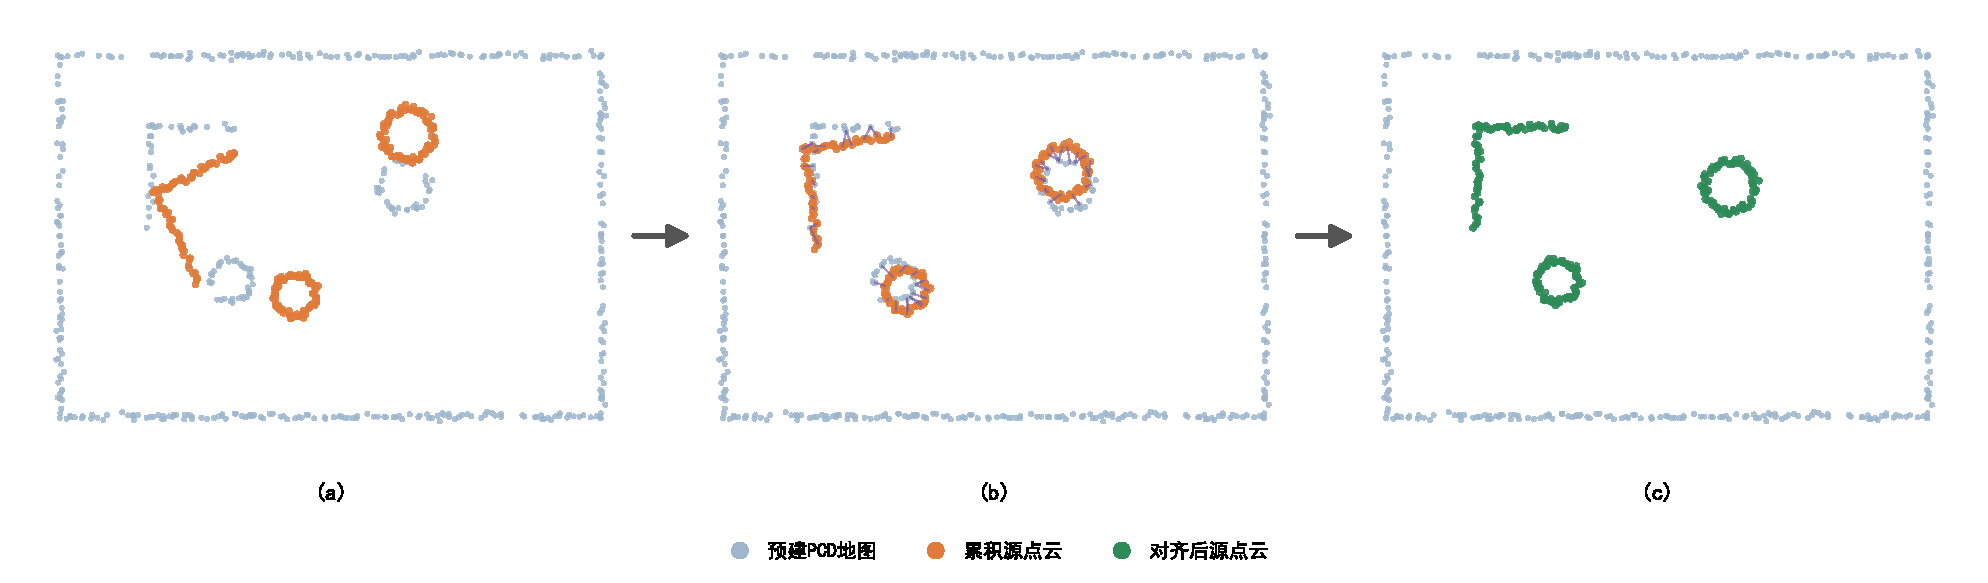
\includegraphics[width=\linewidth]{pic/两阶段ICP初始对齐.pdf}
  \caption{两阶段初始对齐过程示意}
  \label{fig:icp_align}
\end{figure}

\subsection{地图约束下的在线定位更新}
完成初始对齐后，系统进入逐帧定位阶段。每当激光点云与IMU数据完成时间同步，状态估计器首先根据IMU序列进行状态传播，并对当前帧点云进行运动畸变补偿；随后，将去畸变点云变换到地图坐标系，在预建地图中搜索近邻点并拟合局部平面，构造点到平面的残差；最后，通过迭代误差状态卡尔曼滤波更新机器人位姿、速度和IMU偏置。由于纯定位模式下地图保持固定，激光量测始终约束在同一全局地图坐标系内，输出位姿也自然具有全局一致性。

从算法结构看，该流程可抽象为以下步骤：

（1）加载预建点云地图，对地图点云进行降采样，并构建空间索引。

（2）利用启动阶段IMU数据估计重力方向、陀螺仪偏置和初始协方差，同时累积若干帧激光点云作为初始配准源点云。

（3）若预建地图有效，则以近似初值执行ICP配准，将得到的修正变换写入滤波器状态，并将定位状态标记为可用；若预建地图为空或点数不足，则退化为普通SLAM模式。

（4）在每一帧同步后的激光和IMU数据到来时，先进行IMU传播和点云去畸变，再将当前帧点云降采样并变换到地图坐标系。

（5）在地图索引中搜索近邻点并拟合局部平面，构造点到平面残差和量测雅可比，通过迭代卡尔曼滤波更新状态。若系统处于混合建图模式，则将满足条件的新观测增量并入地图。

\subsection{纯定位模式与混合建图模式}
\label{subsec:loc_mapping_modes}
根据地图是否随在线观测更新，本文方法可分为纯定位模式和混合建图模式。纯定位模式仅使用预建地图进行位姿估计，不将当前帧点云写入地图。这种模式适用于已经完成地图采集、作业路线相对固定的场景，能够避免动态障碍物、临时设备或点云噪声污染全局地图。混合建图模式则在完成初始定位并稳定运行后允许地图增量更新，适用于预建地图不完整或机器人需要探索扩展区域的场景。此时新采集点云会在当前地图坐标系下并入地图，使扩展区域与原始地图保持同一坐标基准。

需要注意的是，本文所述重定位主要指系统启动或任务重启时基于近似初值的地图坐标恢复，而不是完全无先验的全局定位。由于ICP属于局部优化方法，初始位姿误差过大、环境几何重复、视场内有效结构过少或预建地图与当前环境差异过大时，配准可能收敛到错误局部最优。因此，在实际部署中应结合机器人停靠点、人工给定初值、二维码/定位桩、轮速里程计或上层任务先验提供合理初始位姿。同时，机器人应在地图加载和初始化期间保持静止，以保证IMU初始化和点云累积质量。
\section{仿真实验与结果分析}
为验证本章所述基于FAST-LIO2的预建地图定位方法，本节在Gazebo仿真环境中设置三类场景，从定位精度、初始对齐鲁棒性与计算开销三个维度对纯定位、混合建图和纯里程计模式进行比较。

% ──────────────────────────────────────────────────────────────────────────────
\subsection{仿真平台与实验设置}
% ──────────────────────────────────────────────────────────────────────────────
\subsubsection{仿真环境与硬件配置}
实验采用Gazebo 11与ROS Noetic搭建测试平台，仿真Livox MID-360激光雷达（非重复扫描，帧率$10\,\mathrm{Hz}$）和$100\,\mathrm{Hz}$ IMU，二者通过仿真插件生成带时间戳的点云与惯性测量。仿真底盘按预设轨迹运动，定位算法仅使用激光雷达与IMU数据，不使用Gazebo真值参与状态估计。Gazebo通过\texttt{model\_states}话题或P3D插件输出的机器人位姿仅作为评价基准，用于计算绝对轨迹误差（Absolute Trajectory Error, ATE）与相对位姿误差（Relative Pose Error, RPE）。

实验在Intel i7-11800H CPU（8核16线程，2.3 GHz）、16 GB内存的笔记本电脑上运行，操作系统为Ubuntu 20.04。FAST-LIO2定位算法运行于单独的ROS节点，与Gazebo仿真器并行但独立计算，不占用仿真器资源。

\subsubsection{实验场景设计}
为覆盖不同几何结构特征与定位退化条件，设计三个典型仿真场景，其参数如表~\ref{tab:exp_scenarios}所示。

\begin{table}[htbp]
\centering
\caption{仿真实验场景参数}
\label{tab:exp_scenarios}
\begin{tabular}{lcccc}
\toprule
\textbf{场景名称} & \textbf{环境特征} & \textbf{轨迹时长 (s)} & \textbf{帧数} & \textbf{里程 (m)} \\
\midrule
走廊          & 长直通道，几何退化敏感            & 145   & $\sim$2900  & 78  \\
迷宫          & 结构丰富，多转弯，特征密集        & 180   & $\sim$3600  & 112 \\
圆柱体林      & 稀疏重复结构，对称性干扰          & 160   & $\sim$3200  & 95  \\
\bottomrule
\end{tabular}
\end{table}

走廊场景模拟大型厂房或地下设施内部的长直通道，墙面平行且特征单一，易产生沿走廊方向的定位退化；迷宫场景包含多个拐角与分支路径，几何约束充分，对应复杂室内环境；圆柱体林场景由若干圆柱体障碍物随机分布构成，考察算法在重复结构下的鲁棒性。三个仿真场景的Gazebo模型如图~\ref{fig:exp_gazebo}所示。每个场景均以匀速或变速方式完成完整轨迹采集，雷达频率10 Hz，单帧点云约8000--12000点。

\begin{figure}[htbp]
  \centering
  \subfloat[走廊场景]{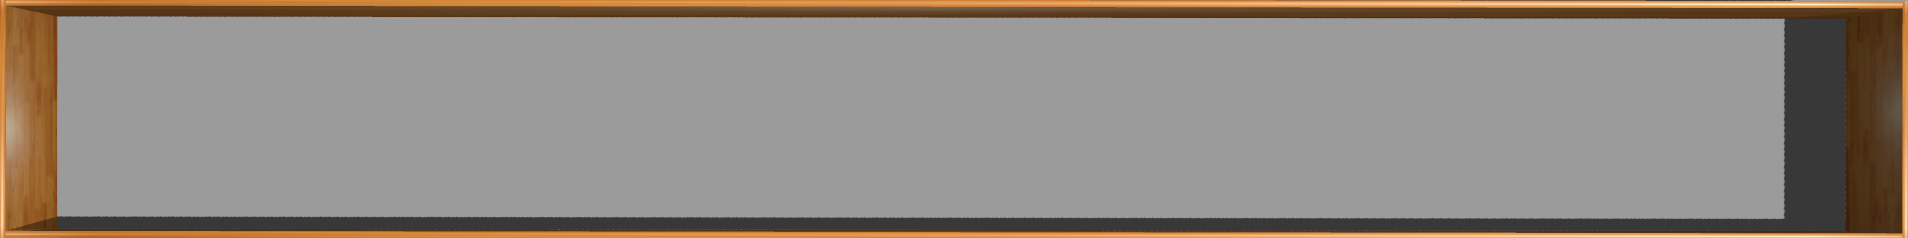
\includegraphics[width=0.78\textwidth]{pic/gazebo走廊.png}\label{fig:gazebo_corridor}}\\
  \vspace{4pt}
  \subfloat[迷宫场景]{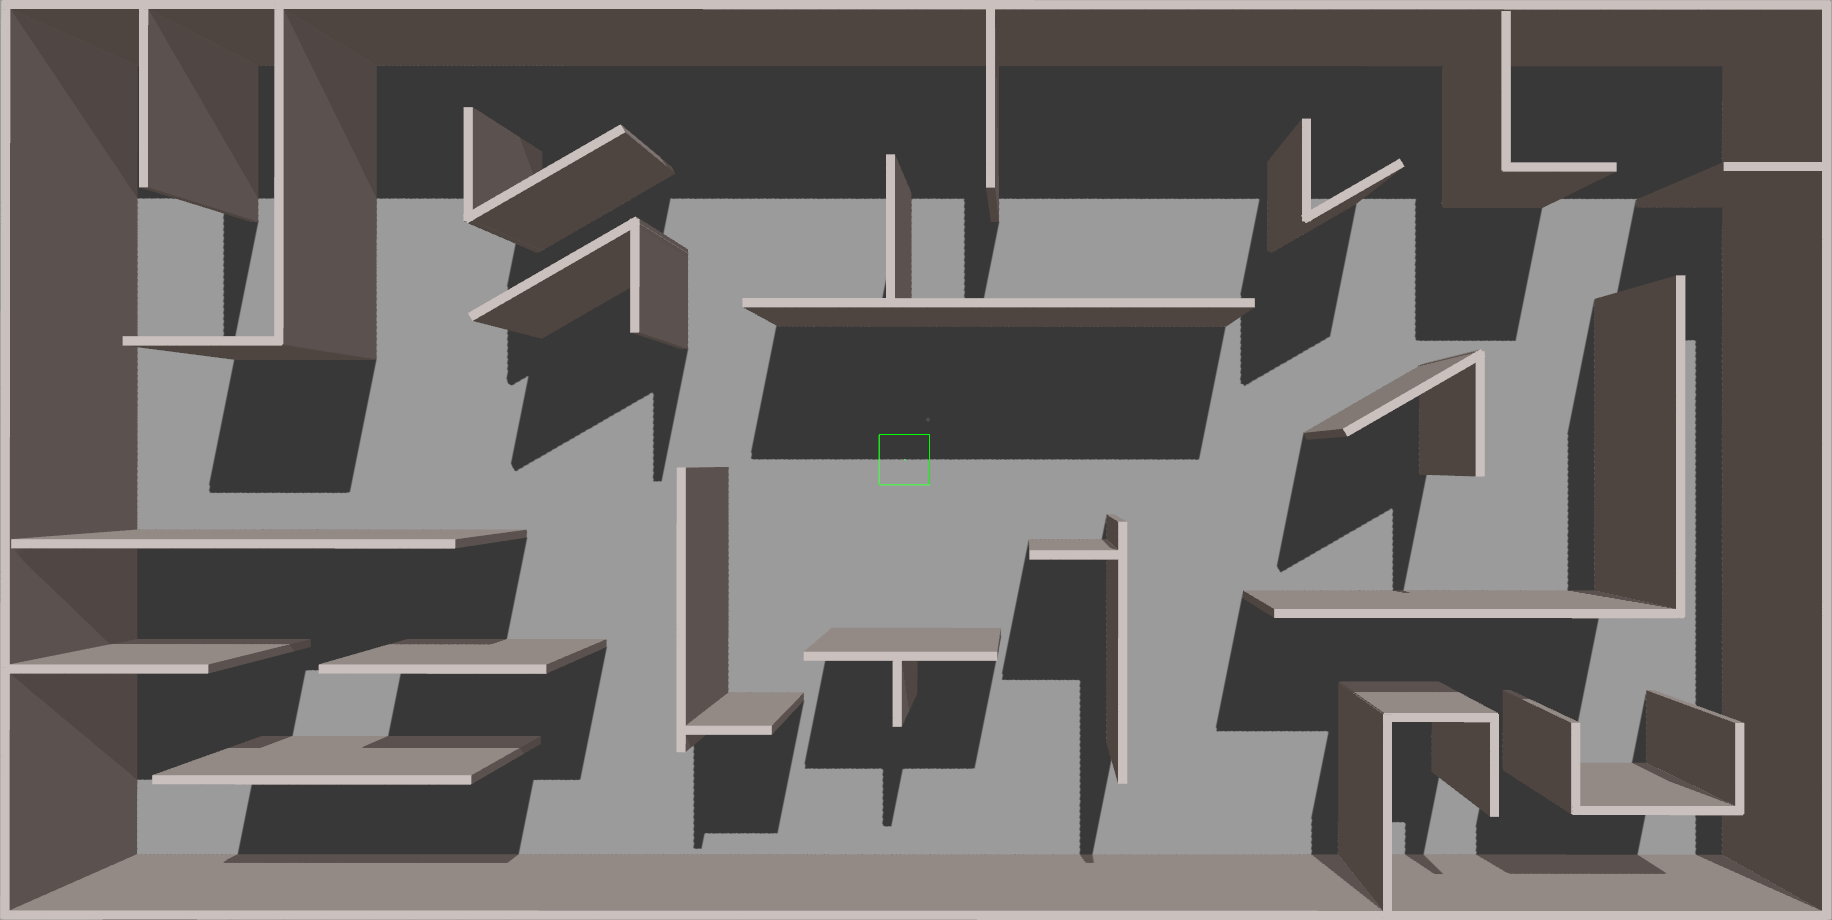
\includegraphics[width=0.55\textwidth]{pic/gazebo迷宫.png}\label{fig:gazebo_maze}}
  \hfill
  \subfloat[圆柱体林场景]{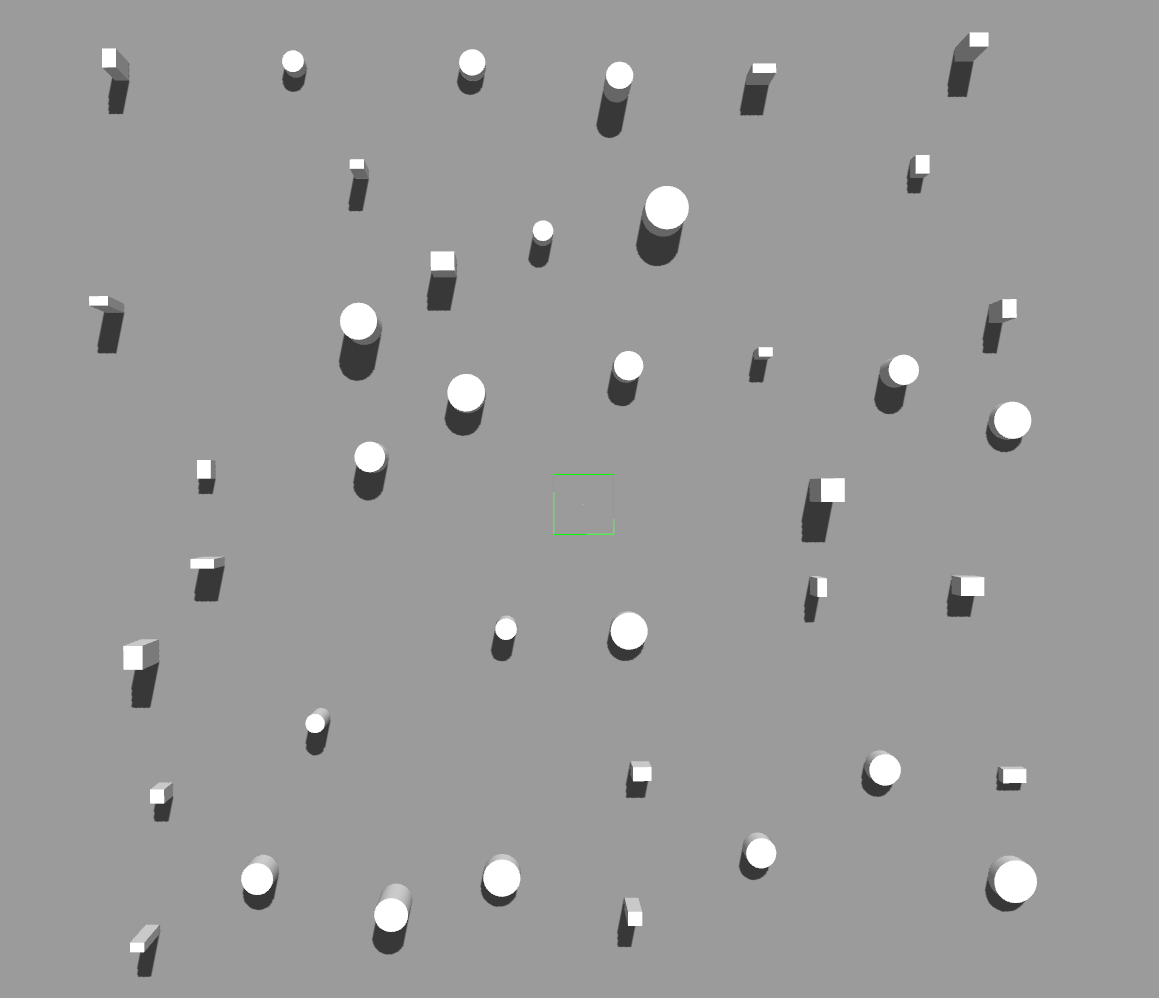
\includegraphics[width=0.40\textwidth]{pic/gazebo柱体.png}\label{fig:gazebo_cylinder}}
  \caption{三类仿真实验场景的Gazebo环境模型}
  \label{fig:exp_gazebo}
\end{figure}

\subsubsection{实验流程与评价指标}
实验流程分为两阶段：第一阶段，机器人在各场景以SLAM模式（无预建地图）运行，累积点云并构建全局地图，保存为PCD格式；第二阶段，加载预建地图，在纯定位模式或混合建图模式下重复相同轨迹，记录估计位姿与真值位姿，离线计算误差指标。

定位精度评价采用如下指标：
\begin{itemize}
    \item \textbf{绝对轨迹误差（ATE）}：估计轨迹与真值轨迹在相同时间戳下的欧氏距离，统计均方根误差（RMSE）、均值与最大值。ATE反映全局定位精度。
    \item \textbf{相对位姿误差（RPE）}：相邻时刻位姿变化的估计值与真值之间的差异，分别统计平移误差（m/m）与旋转误差（deg/m）。RPE反映局部一致性与漂移速率。
\end{itemize}
误差计算采用开源工具\texttt{evo}\footnote{\url{https://github.com/MichaelGrupp/evo}}，自动对齐时间戳并生成统计报告。实时性评价通过ROS节点内部计时记录单帧处理耗时，并统计各模块占比。

% ──────────────────────────────────────────────────────────────────────────────
\subsection{定位精度评估}
% ──────────────────────────────────────────────────────────────────────────────
本实验对比三种运行模式在三个场景下的定位精度：（1）\textbf{纯定位模式}：加载预建地图，地图固定不更新（对应\texttt{update\_tree\_frame = -1}）；（2）\textbf{混合建图模式}：加载预建地图，80帧后开启增量更新（对应\texttt{update\_tree\_frame = 80}）；（3）\textbf{纯里程计模式}：不加载预建地图，仅依赖FAST-LIO2里程计，作为漂移对照基准。

\subsubsection{轨迹对比}
图~\ref{fig:exp_trajectory}给出了三个场景下估计轨迹与真值轨迹的叠加结果。两种地图约束模式的轨迹与真值轨迹基本重合，而纯里程计轨迹的偏差随运行时间逐渐累积。走廊场景中，纯里程计轨迹沿通道方向出现明显偏移，与长直通道内该方向几何约束不足的特点一致；迷宫场景转角与几何结构较丰富，三种模式的轨迹偏差均相对较小；圆柱体林场景由于重复结构造成近邻匹配存在歧义，纯里程计轨迹出现局部波动。

\begin{figure}[htbp]
  \centering
  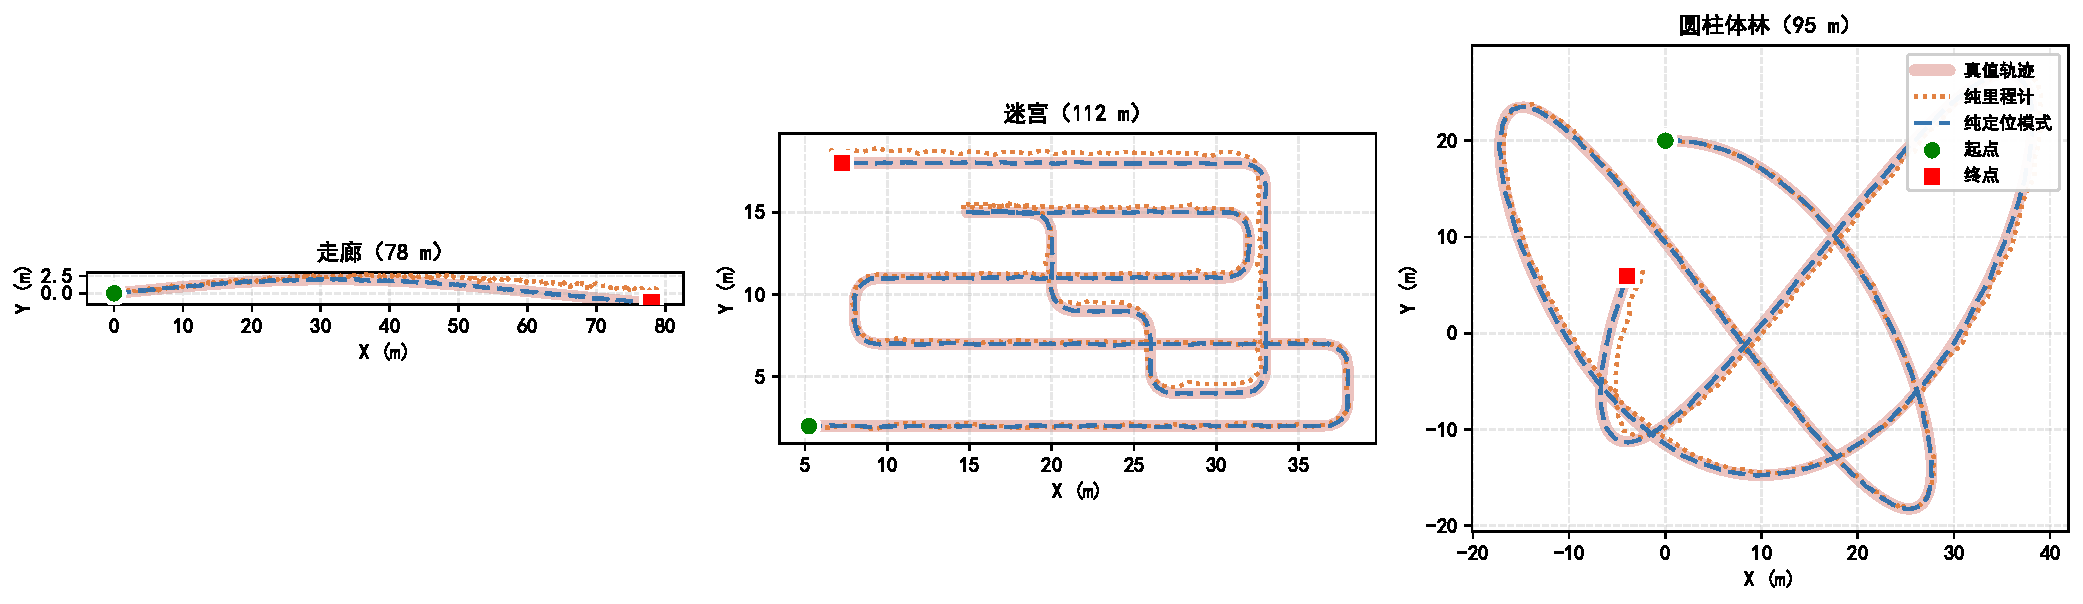
\includegraphics[width=\linewidth]{pic/实验_轨迹对比图.pdf}
  \caption{三场景轨迹对比：估计轨迹与真值叠加}
  \label{fig:exp_trajectory}
\end{figure}

\subsubsection{绝对轨迹误差统计}
表~\ref{tab:ate_results}给出了ATE统计结果。两种地图约束模式的定位精度均显著优于纯里程计模式：以走廊场景为例，ATE-RMSE由纯里程计的$0.410\,\mathrm{m}$降至纯定位模式的$0.082\,\mathrm{m}$和混合建图模式的$0.071\,\mathrm{m}$，降幅分别为$80.0\%$和$82.7\%$；迷宫与圆柱体林场景的相应降幅分别达到$77.4\%$和$79.3\%$。这说明预建地图提供的全局几何约束能够有效抑制里程计的累积漂移。

在两种地图约束模式之间，混合建图模式的ATE-RMSE在三个场景中均略低于纯定位模式，分别由$0.082\,\mathrm{m}$、$0.046\,\mathrm{m}$和$0.061\,\mathrm{m}$降至$0.071\,\mathrm{m}$、$0.043\,\mathrm{m}$和$0.058\,\mathrm{m}$，改善幅度在$5\%$至$13\%$之间。其原因在于增量更新补充了预建地图中因视角遮挡或采样稀疏而缺失的局部结构，使近邻匹配可用的平面约束更充分；但由于预建地图已提供主要几何约束，该项改善量明显小于地图约束相对纯里程计带来的提升。就场景差异而言，迷宫场景误差最低（纯定位$0.046\,\mathrm{m}$），走廊场景误差最高（纯定位$0.082\,\mathrm{m}$），圆柱体林场景介于二者之间（纯定位$0.061\,\mathrm{m}$），该顺序与迷宫转角丰富、约束方向完备，而长直走廊沿通道方向约束较弱、圆柱体林存在重复结构歧义的场景特征相符。三个场景中最大ATE均不超过$0.16\,\mathrm{m}$，可满足后续路径规划与运动控制对位姿输入的精度需求。

\begin{table}[htbp]
\centering
\caption{绝对轨迹误差（ATE）统计结果}
\label{tab:ate_results}
\begin{tabular}{lcccc}
\toprule
\textbf{场景} & \textbf{模式} & \textbf{RMSE (m)} & \textbf{Mean (m)} & \textbf{Max (m)} \\
\midrule
\multirow{3}{*}{走廊}   & 纯定位      & 0.082  & 0.076  & 0.158 \\
                        & 混合建图    & 0.071  & 0.065  & 0.142 \\
                        & 纯里程计    & 0.410  & 0.385  & 0.782 \\
\midrule
\multirow{3}{*}{迷宫}   & 纯定位      & 0.046  & 0.042  & 0.095 \\
                        & 混合建图    & 0.043  & 0.039  & 0.088 \\
                        & 纯里程计    & 0.190  & 0.175  & 0.398 \\
\midrule
\multirow{3}{*}{圆柱体林} & 纯定位    & 0.061  & 0.056  & 0.125 \\
                        & 混合建图    & 0.058  & 0.053  & 0.118 \\
                        & 纯里程计    & 0.280  & 0.262  & 0.545 \\
\bottomrule
\end{tabular}
\end{table}

图~\ref{fig:exp_accuracy}左侧给出迷宫场景的绝对位姿误差（Absolute Pose Error, APE）时间序列，右侧给出三个场景的ATE分布箱线图。两种地图约束模式的APE曲线在整个运行时段内保持平稳，未出现随时间单调增长的趋势；纯里程计模式的APE则随里程累积而抬升。箱线图显示，地图约束模式的误差分布区间更窄、离群点更少，表明其定位输出在时间上更为稳定。

\begin{figure}[htbp]
  \centering
  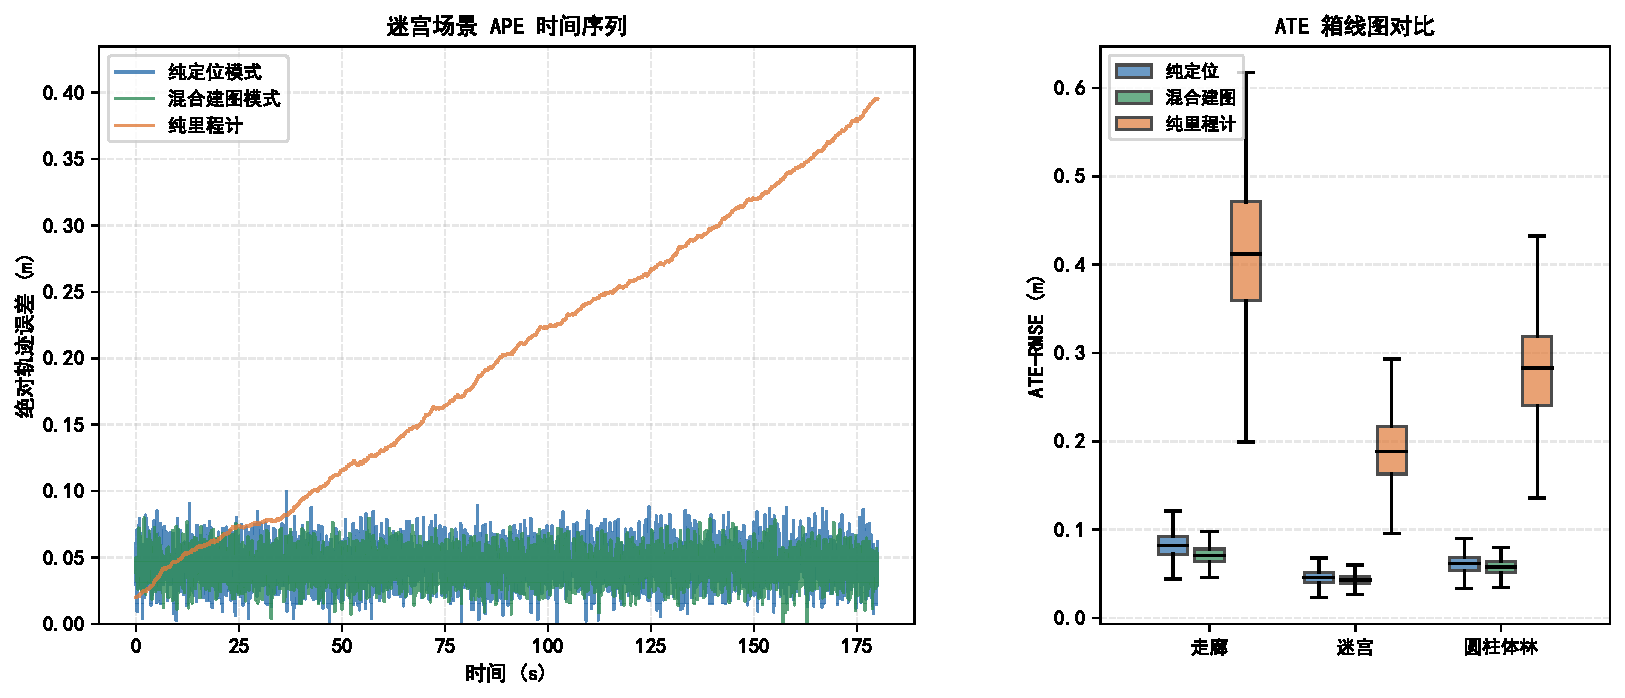
\includegraphics[width=\linewidth]{pic/实验_定位精度对比图.pdf}
  \caption{定位精度对比：APE时间序列（左）与ATE箱线图（右）}
  \label{fig:exp_accuracy}
\end{figure}

\subsubsection{相对位姿误差}
表~\ref{tab:rpe_results}给出了RPE统计结果。平移RPE以单位里程的平移偏差衡量局部轨迹一致性，旋转RPE用于衡量单位里程的姿态偏差，二者反映漂移速率而不受全局对齐方式影响。三个场景中，地图约束模式的平移RPE均不超过$0.0012\,\mathrm{m/m}$，旋转RPE均不超过$0.028\,\mathrm{deg/m}$；纯里程计模式的相应指标则达到$0.0025$--$0.0052\,\mathrm{m/m}$与$0.048$--$0.092\,\mathrm{deg/m}$，约为地图约束模式的$3$至$4$倍。以走廊场景为例，混合建图模式的平移RPE为$0.0010\,\mathrm{m/m}$，仅为纯里程计模式$0.0052\,\mathrm{m/m}$的$19.2\%$。RPE与ATE的趋势一致，说明地图约束模式的精度提升来自漂移速率本身的降低，而非全局对齐带来的表观改善。

\begin{table}[htbp]
\centering
\caption{相对位姿误差（RPE）统计结果}
\label{tab:rpe_results}
\begin{tabular}{lcccc}
\toprule
\textbf{场景} & \textbf{模式} & \textbf{平移RPE (m/m)} & \textbf{旋转RPE (deg/m)} \\
\midrule
\multirow{3}{*}{走廊}   & 纯定位      & 0.0012  & 0.028  \\
                        & 混合建图    & 0.0010  & 0.025  \\
                        & 纯里程计    & 0.0052  & 0.092  \\
\midrule
\multirow{3}{*}{迷宫}   & 纯定位      & 0.0008  & 0.019  \\
                        & 混合建图    & 0.0007  & 0.017  \\
                        & 纯里程计    & 0.0025  & 0.048  \\
\midrule
\multirow{3}{*}{圆柱体林} & 纯定位    & 0.0010  & 0.023  \\
                        & 混合建图    & 0.0009  & 0.021  \\
                        & 纯里程计    & 0.0035  & 0.065  \\
\bottomrule
\end{tabular}
\end{table}

% ──────────────────────────────────────────────────────────────────────────────
\subsection{初始对齐（ICP）有效性}
% ──────────────────────────────────────────────────────────────────────────────
本节按“初值扰动—ICP收敛—位姿误差”的流程评估两阶段初始对齐策略。以迷宫场景为例，对配置参数\texttt{approximate\_init\_pose}施加不同幅度的平移与旋转扰动，并在每组扰动条件下重复运行，记录收敛成功率、迭代次数及配准RMSE。成功判据统一取为“在最大迭代次数内残差降至设定阈值以下，且最终位姿误差低于阈值”，扰动网格与重复次数在实验前固定，以保证各组条件可比。

\subsubsection{收敛成功率}
图~\ref{fig:exp_icp}左侧的成功率热力图给出了平移与旋转扰动对ICP收敛的联合影响。结果表明，初值越接近真实位姿，点云间的最近邻对应越可靠，收敛成功率越高；随着平移或旋转扰动增大，成功率逐步下降，失败样本主要表现为陷入错误局部最优或达到迭代上限。热力图中平移扰动小于$1\,\mathrm{m}$、旋转扰动小于$20^{\circ}$的区域成功率保持在较高水平，可作为该场景下初始位姿给定精度的参考范围。

\begin{figure}[htbp]
  \centering
  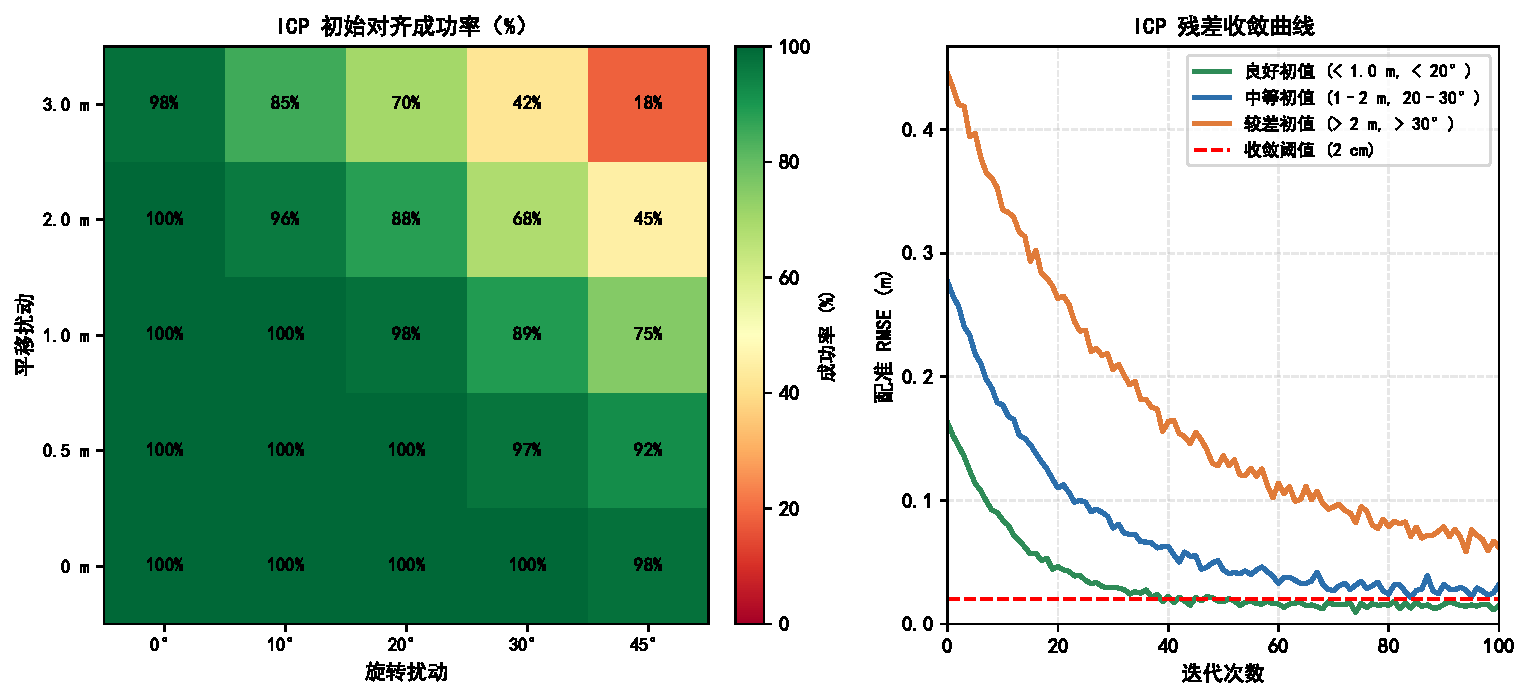
\includegraphics[width=\linewidth]{pic/实验_ICP对齐分析图.pdf}
  \caption{ICP初始对齐分析：成功率热力图（左）与收敛曲线（右）}
  \label{fig:exp_icp}
\end{figure}

\subsubsection{收敛速度与配准精度}
图~\ref{fig:exp_icp}右侧给出不同初值等级下的ICP残差收敛曲线，表~\ref{tab:icp_results}给出对应的成功率、平均迭代次数与配准RMSE。初值良好（平移扰动小于$1\,\mathrm{m}$、旋转扰动小于$20^{\circ}$）时，成功率为$99.5\%$，平均迭代$25$次即收敛，配准RMSE为$2.1\,\mathrm{cm}$；初值中等（平移$1$--$2\,\mathrm{m}$、旋转$20^{\circ}$--$30^{\circ}$）时，成功率降至$88.3\%$，平均迭代次数增至$52$次，配准RMSE增至$3.2\,\mathrm{cm}$；初值较差（平移大于$2\,\mathrm{m}$、旋转大于$30^{\circ}$）时，成功率仅为$51.7\%$，平均迭代次数达$78$次，配准RMSE为$4.6\,\mathrm{cm}$。可见随扰动增大，残差下降速度变缓、最终配准精度下降，且迭代次数的增幅大于精度的降幅，说明失败样本多因初始对应关系错误而在迭代上限附近才被判定，而非缓慢收敛至正确解。结合迷宫场景存在多处相似转角结构可以解释部分异常收敛：当初值偏差超过相邻相似结构的间距时，最近邻搜索会建立跨结构的错误对应，使ICP收敛到错误位姿。因此在实际部署中，应将近似初始位姿的给定精度控制在平移$1\,\mathrm{m}$、旋转$20^{\circ}$以内，以保证启动重定位的可靠性。

\begin{table}[htbp]
\centering
\caption{ICP初始对齐性能}
\label{tab:icp_results}
\begin{tabular}{lccc}
\toprule
\textbf{扰动等级} & \textbf{成功率 (\%)} & \textbf{平均迭代次数} & \textbf{配准RMSE (cm)} \\
\midrule
良好 ($<$ 1 m, $<$ 20°)     & 99.5   & 25   & 2.1  \\
中等 (1–2 m, 20–30°)       & 88.3   & 52   & 3.2  \\
较差 ($>$ 2 m, $>$ 30°)    & 51.7   & 78   & 4.6  \\
\bottomrule
\end{tabular}
\end{table}

% ──────────────────────────────────────────────────────────────────────────────
\subsection{实时性与计算开销}
% ──────────────────────────────────────────────────────────────────────────────
\subsubsection{模块耗时分解}
实时性评价记录单帧处理总耗时及IMU传播与降采样、近邻匹配、IESKF更新和地图增量维护等模块耗时。图~\ref{fig:exp_timing}和表~\ref{tab:timing_results}给出了统计结果。由于混合建图模式包含地图增量更新开销，表中数据取自该模式，即三种运行模式中计算负担最重的情形。从模块占比看，近邻匹配是主要开销来源，在走廊、迷宫和圆柱体林场景中分别占单帧总耗时的$45.9\%$、$50.6\%$和$48.8\%$，这与该步骤需在ikd-Tree上为每个降采样点执行近邻查询有关；IESKF更新占比约$20\%$--$25\%$，IMU传播与降采样、地图增量维护的开销相对较小。

\begin{figure}[htbp]
  \centering
  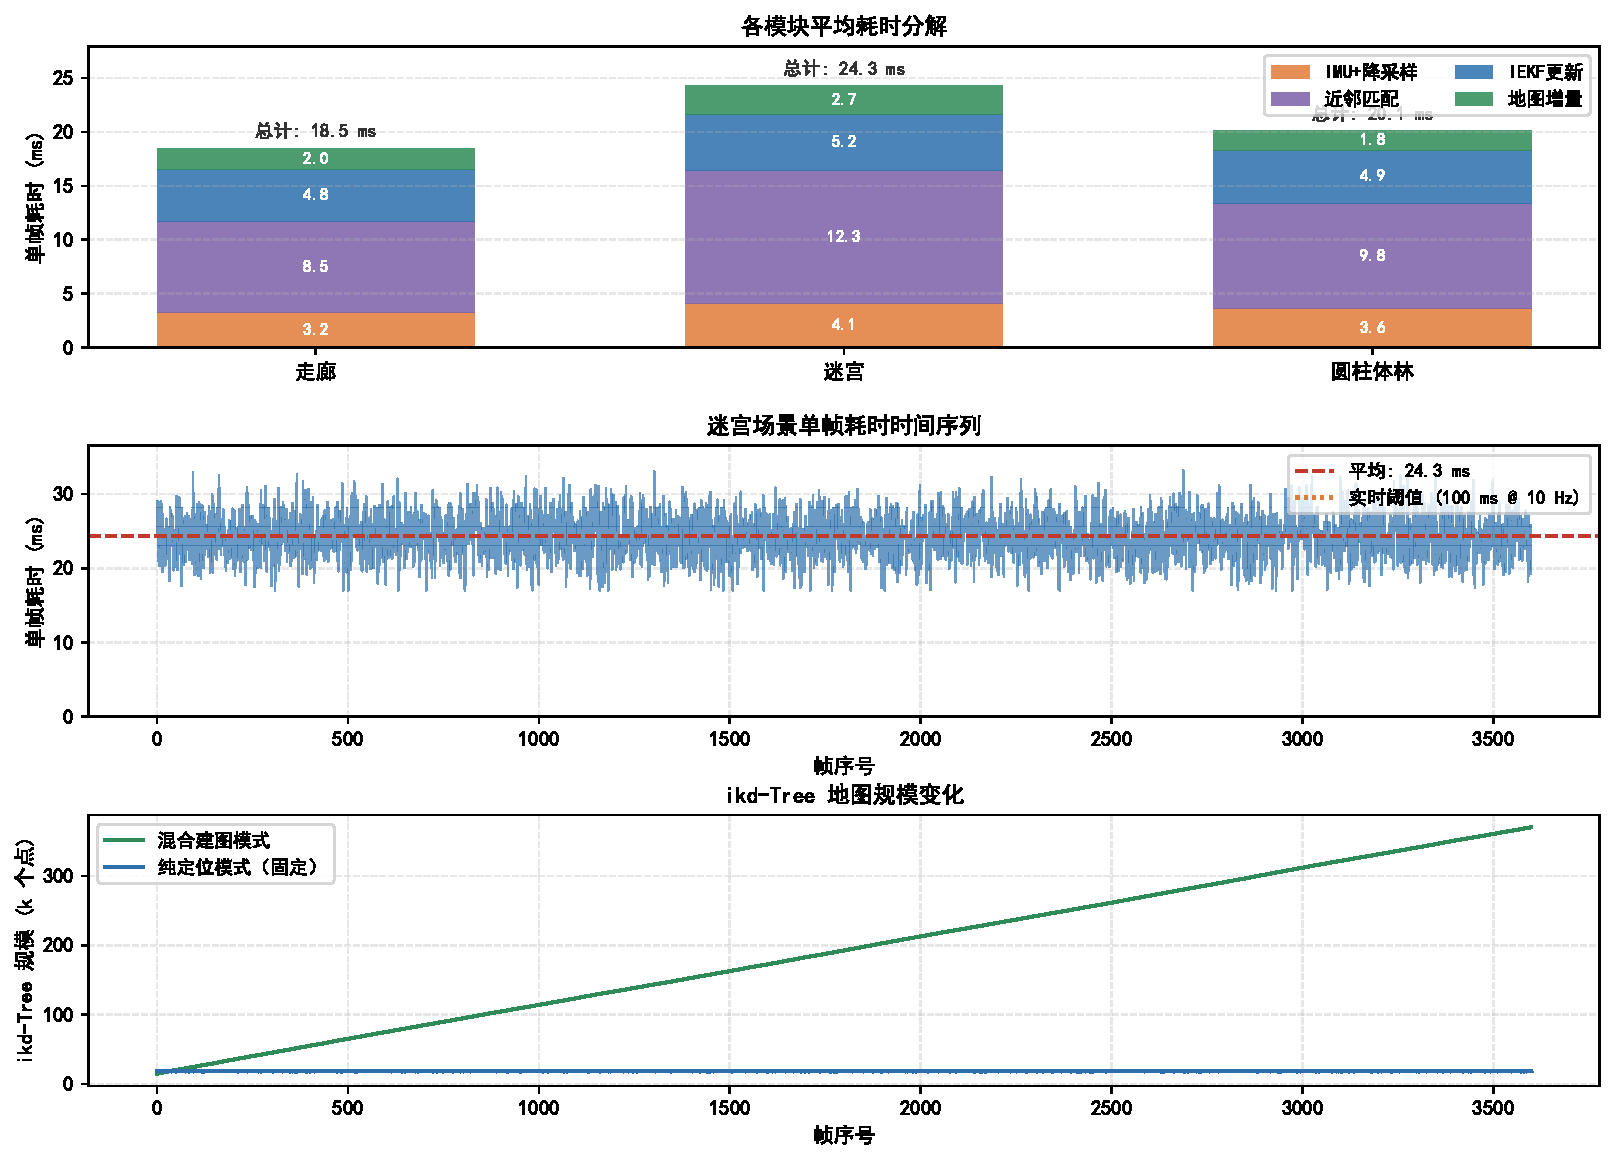
\includegraphics[width=\linewidth]{pic/实验_实时性能分析图.pdf}
  \caption{实时性能分析：模块耗时分解（上）、单帧耗时序列（中）、ikd-Tree规模变化（下）}
  \label{fig:exp_timing}
\end{figure}

三个场景的单帧平均总耗时分别为$18.5\,\mathrm{ms}$、$24.3\,\mathrm{ms}$和$20.1\,\mathrm{ms}$，对应的可达处理帧率分别为$54\,\mathrm{Hz}$、$41\,\mathrm{Hz}$和$50\,\mathrm{Hz}$，均远高于激光雷达$10\,\mathrm{Hz}$的输出频率，即单帧耗时仅占$100\,\mathrm{ms}$雷达周期的$18.5\%$--$24.3\%$。迷宫场景耗时最高，与其点云特征密集、有效近邻点数量较多相符；走廊场景几何结构单一，参与匹配的点数较少，耗时最低。由于混合建图模式下的高负载情形仍保留约四倍的周期余量，定位节点可在该计算平台上稳定实时运行，并为同一平台上的感知与规划模块留有算力空间。

\begin{table}[htbp]
\centering
\caption{混合建图模式下各模块计算耗时与帧率统计}
\label{tab:timing_results}
\begin{tabular}{lcccccc}
\toprule
\textbf{场景} & \textbf{IMU+降采样} & \textbf{近邻匹配} & \textbf{IEKF更新} & \textbf{地图增量} & \textbf{总耗时} & \textbf{帧率} \\
              & \textbf{(ms)}       & \textbf{(ms)}    & \textbf{(ms)}    & \textbf{(ms)}    & \textbf{(ms)}  & \textbf{(Hz)} \\
\midrule
走廊          & 3.2   & 8.5   & 4.8  & 2.0  & 18.5  & 54  \\
迷宫          & 4.1   & 12.3  & 5.2  & 2.7  & 24.3  & 41  \\
圆柱体林      & 3.6   & 9.8   & 4.9  & 1.8  & 20.1  & 50  \\
\bottomrule
\end{tabular}
\end{table}

\subsubsection{单帧耗时波动与地图规模}
图~\ref{fig:exp_timing}中图给出单帧耗时序列，下图给出ikd-Tree的地图规模变化。单帧耗时在平均值附近小幅波动，未出现超过雷达周期的突发峰值；耗时相对较高的片段集中在机器人转弯和进入新区域时，此时视场内结构变化较快、有效近邻点增多。对比两种模式可见，纯定位模式下地图规模固定，耗时序列的波动幅度更小；混合建图模式下地图节点数随增量更新持续增长，但单帧耗时并未随之同比例上升。这说明ikd-Tree的局部重构与树上降采样机制将新增点合并到已有体素中，使近邻查询的实际搜索范围保持在局部区域，从而把地图规模增长对计算开销的影响控制在有限范围内。

% ──────────────────────────────────────────────────────────────────────────────
\subsection{实验结果讨论}
% ──────────────────────────────────────────────────────────────────────────────
综合上述实验结果，可得到以下四点结论。第一，预建地图提供的全局几何约束能够有效抑制里程计漂移。两种地图约束模式的ATE-RMSE相对纯里程计模式下降$77\%$以上，且RPE呈现同样的趋势，说明改善来自漂移速率的降低，而非全局轨迹对齐造成的表观效果。第二，两种地图约束模式的精度差异有限。混合建图模式的ATE-RMSE比纯定位模式低$5\%$至$13\%$，改善来自对预建地图局部缺失结构的补充；由于主要几何约束已由预建地图提供，该增益远小于地图约束相对纯里程计的提升。第三，启动重定位的可靠性取决于近似初值精度。当平移扰动小于$1\,\mathrm{m}$、旋转扰动小于$20^{\circ}$时，ICP收敛成功率达$99.5\%$、配准RMSE为$2.1\,\mathrm{cm}$；扰动超过$2\,\mathrm{m}$或$30^{\circ}$后成功率降至$51.7\%$，主要失败原因是相似结构间建立了错误的最近邻对应。第四，算法满足实时性要求。混合建图模式下单帧平均总耗时不超过$24.3\,\mathrm{ms}$，约为雷达周期的四分之一，且地图规模增长未引起耗时同比例上升。

在模式选择上，纯定位模式避免在线观测污染固定地图，适合环境相对稳定的重复作业任务；混合建图模式可补充地图缺失结构并获得略高的精度，适合环境存在局部变化的场景，但需配合动态目标剔除以避免错误观测破坏地图一致性。需要说明的是，本节结论建立在Gazebo仿真条件下，其传感器噪声模型与真实硬件仍存在差异，机械振动、动态遮挡和长期环境变化的影响未能完全反映；上述定位方法在典型工业与特种作业场景中的表现，将结合第6章的实物实验进一步验证。

\section{本章小结}
本章围绕移动机器人定位需求，研究了基于FAST-LIO2的激光里程计定位算法。首先介绍了SLAM系统的基本架构和技术分类，分析了基于滤波器、基于图优化以及紧耦合激光惯性SLAM方法的特点。随后重点阐述FAST-LIO2的核心原理，包括IMU状态传播、激光点云运动畸变补偿、直接点到地图残差、流形迭代卡尔曼滤波以及ikd-Tree增量地图维护机制。

在此基础上，本章说明了面向预建PCD地图的定位与启动重定位流程。系统通过加载预建地图构建空间索引，以近似初始位姿和ICP完成地图坐标系下的初始对齐，并在后续运行中利用FAST-LIO2的点到平面量测更新持续输出全局位姿。通过区分纯定位模式和混合建图模式，所述方法能够在固定地图重复作业和地图扩展两类任务之间切换，为后续路径规划、障碍物检测和导航控制模块提供稳定的位姿基础。

Gazebo仿真实验在走廊、迷宫和圆柱体林三类场景中验证了上述方法。两种地图约束模式的ATE-RMSE相对纯里程计模式下降$77\%$以上，最大绝对轨迹误差不超过$0.16\,\mathrm{m}$，相对位姿误差呈现一致趋势，表明预建地图约束有效抑制了累积漂移；在平移扰动小于$1\,\mathrm{m}$、旋转扰动小于$20^{\circ}$的初值条件下，ICP初始对齐成功率为$99.5\%$，配准RMSE为$2.1\,\mathrm{cm}$；混合建图模式下单帧平均处理耗时不超过$24.3\,\mathrm{ms}$，约为激光雷达输出周期的四分之一，满足实时定位需求。

从算法特点与适用性来看，相较于仅依赖轮式里程计或AMCL粒子滤波的二维定位方法，基于FAST-LIO2的三维激光惯性定位具有以下优势。首先，三维点云能够直接利用墙面、设备支架、电缆沟边缘和立体障碍物等空间结构，在平面纹理不明显或二维激光可见特征不足时仍可提供较强约束。其次，IMU传播为高频状态估计和点云去畸变提供支撑，可提升机器人在转弯、加减速和短时遮挡条件下的定位连续性。再次，直接点到地图配准减少了特征提取阈值对不同雷达型号和扫描模式的依赖，有利于系统在不同传感器平台上的迁移。该方法也存在一定局限：其一，FAST-LIO2本质上仍是局部里程计框架，若脱离预建地图或回环后端，长距离运行会产生漂移，本文通过固定预建地图定位减轻该问题，但地图本身的质量会直接影响定位效果；其二，激光几何约束依赖足够丰富的空间结构，在长直走廊、开阔区域、单一大平面或近距离遮挡严重场景中可能出现退化；其三，该启动重定位策略依赖近似初值和ICP收敛性，不适合直接处理完全未知初始位置。针对上述问题，后续可进一步引入全局点云描述子、回环检测或多源传感器辅助定位，以提升全局重定位能力和长期运行稳定性。


\chapter{移动机器人障碍检测与环境感知算法设计}
\section{引言}
自主移动机器人广泛应用于制造、仓储、施工、能源设施维护和应急救援等工业与特种作业场景，工作环境通常由设备、货架、作业人员、车辆、其他移动机器人以及临时堆放物等静态和动态障碍物共同构成。要确保机器人在这种复杂动态环境中安全、平稳地导航并完成作业任务，需要实时、准确地感知周围环境，为机器人定位、地图更新和路径规划提供可靠信息。

移动机器人的机载检测与跟踪面临三个挑战。首先，有限的机载计算资源难以支撑对GPU算力要求较高的学习类检测方法\textsuperscript{\cite{10372107,9157234}}；在计算约束下，处理规模庞大的点云数据或部署重型激光雷达系统均不现实。其次，适用于小型移动机器人的深度相机量程与视场（Field of View, FOV）有限，障碍物过近或过远时均难以稳定观测，在动态环境中无法及时获取周围障碍物信息。第三，相机输出的深度值存在不可忽略的噪声，不仅会在点云计算环节引入误差、影响障碍物状态估计精度，还会产生高频的假阳性与假阴性结果，导致下游规划器做出错误决策。

对于计算能力受限的小型机器人，可按所用传感器对检测与跟踪方法进行分类，常见的有激光雷达、事件相机、RGB-D相机和深度相机等。激光雷达与深度相机可直接获取空间点云数据以提取三维障碍物；此外，也可基于采集到的图像进行障碍检测，即利用深度图像生成U深度图和V深度图来估计障碍物状态。然而，由于噪声的存在以及动态环境的复杂性，上述两类检测方法均可能出现不同程度的误检。为此，本章研究一种基于图像与点云数据融合的轻量级障碍物检测与跟踪方法，以获得优于单一检测器的检测精度。

该方法结合传统点云检测与图像检测计算效率较高的特点，并通过数据融合减轻两类检测器各自的局限。检测框架可接收图像数据或点云数据，以适应不同的传感器配置，使移动机器人能够实时感知复杂动态环境中的静态和动态障碍物。

本章主要包括以下内容：

（1）介绍K-Means与DBSCAN两类点云聚类方法，分析二者在处理非凸簇、噪声点和未知簇数量时的差异，为点云检测器选择聚类内核提供依据。

（2）构建适合资源受限移动机器人的轻量级障碍物检测框架。分别设计基于U深度图的图像检测器和基于DBSCAN的点云检测器，并通过交并比双向校验与保守融合策略对两类检测结果进行集成，以降低单一检测器在传感器噪声下的误检率。

（3）研究障碍物关联跟踪与动态障碍物识别方法。采用匈牙利算法完成基于特征的跨帧数据关联，利用恒加速度卡尔曼滤波估计障碍物的速度与加速度状态，并针对目标短暂离开视场的情况设计视距外补偿机制；在包围盒速度判据基础上引入点云投票策略，抑制仅依靠速度判别所产生的假阳性结果。

（4）研究面向规划安全约束的局部地图更新方法。以第2章输出的多传感器融合观测和本章的检测跟踪结果为输入，通过Bresenham射线遍历与对数几率贝叶斯更新完成自由空间确认和陈旧占用清理，并在占用层上执行形态学膨胀，为第5章的路径规划提供局部环境表示。

\section{点云聚类算法基础}
\label{sec:clustering}
如前所述，本章的点云检测器需要从第2章得到的三维点云中提取出离散的障碍物个体。由于第2章输出的点云仅是空间中大量无序的三维坐标点，其本身并不包含“哪些点属于同一个障碍物”这一语义信息，因此在进行包围盒估计之前，必须先将属于同一物体的点归并到一起。聚类算法正是完成这一任务的核心手段，它无需预先标注数据，即可依据点在空间中的分布自动划分出若干簇，每一个簇对应一个潜在的障碍物。因此，本节先对聚类算法的基本原理进行介绍，为后续点云检测器的设计奠定基础。

聚类是一类无监督学习方法，旨在根据样本间的相似性将数据集划分为若干簇，使簇内样本尽可能相近、簇间样本尽可能分离。该方法无需预先提供类别标签，能够从数据分布中发现潜在结构，广泛应用于计算机视觉、图像分割与异常检测等领域。本节介绍K-Means与DBSCAN两种典型聚类方法，并结合障碍物点云的分布特征分析其适用性。

\subsection{K-Means聚类}
K-Means通过交替执行样本分配与质心更新，将数据集划分为预先指定的$k$个簇。设数据集包含$m$个$N$维样本$\mathbf{x}_j\in\mathbb{R}^{N}$，第$i$个簇及其质心分别记为$C_i$和$\boldsymbol{\mu}_i$，则其优化目标为
\begin{equation}
    \min_{\{C_i,\boldsymbol{\mu}_i\}_{i=1}^{k}}
    \sum_{i=1}^{k}\sum_{\mathbf{x}_j\in C_i}
    \left\|\mathbf{x}_j-\boldsymbol{\mu}_i\right\|_2^2.
    \label{eq:kmeans_objective}
\end{equation}

算法首先选取$k$个初始质心，再将每个样本分配至欧氏距离最近的质心所对应的簇；随后按下式重新计算各簇质心：
\begin{equation}
    \boldsymbol{\mu}_{i}^{(t+1)}
    =\frac{1}{\left|C_i^{(t)}\right|}
    \sum_{\mathbf{x}_j\in C_i^{(t)}}\mathbf{x}_j,
    \label{eq:kmeans_centroid}
\end{equation}
其中，$t$表示迭代次数，$\left|C_i^{(t)}\right|$表示第$t$次迭代后第$i$个簇中的样本数。样本分配与质心更新交替进行，直至质心变化量或目标函数变化量小于设定阈值。图~\ref{fig:K-Means聚类效果示意图}给出了K-Means对同一数据集进行聚类的示意结果。
\begin{figure}[!htb]
	\centering
	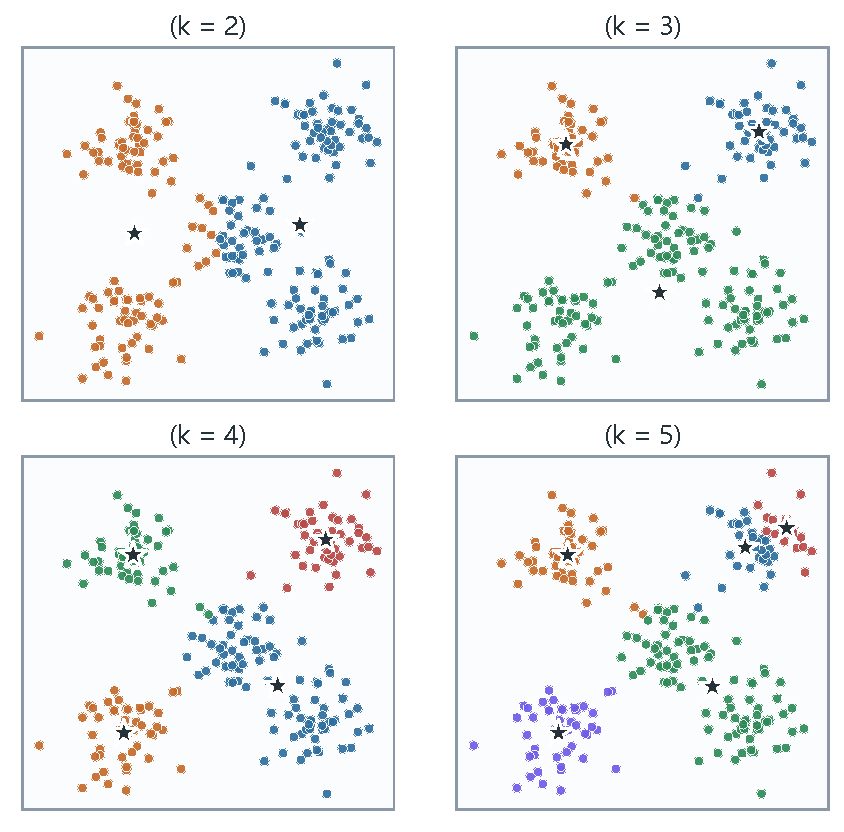
\includegraphics[width=0.72\textwidth]{pic/K-Means聚类效果示意图.pdf}
	\caption{K-Means聚类效果示意图}
	\label{fig:K-Means聚类效果示意图}
\end{figure}
\subsection{DBSCAN聚类}
DBSCAN是一种基于密度的聚类方法，无需预先指定簇数量，能够识别非凸形状的簇并将低密度离群点标记为噪声，因而适合处理形状不规则且含测量噪声的障碍物点云。其基本思想是通过密度可达关系连接高密度区域。对于数据集$D$中的任意点$p$，其$\varepsilon$邻域定义为
\begin{equation}
    N_{\varepsilon}(p)
    =\left\{q\in D\mid \operatorname{dist}(p,q)\leq\varepsilon\right\},
    \label{eq:dbscan_neighborhood}
\end{equation}
其中，$\varepsilon$为邻域半径，$\operatorname{dist}(\cdot)$为距离度量。若$\left|N_{\varepsilon}(p)\right|\geq \mathrm{MinPts}$，则$p$为核心点；位于某一核心点邻域内但自身不满足该条件的样本为边界点；既不是核心点、也不能由任何核心点密度可达的样本才被标记为噪声点。算法从未访问的核心点出发，将其邻域内所有密度可达的样本递归并入同一簇，直至无法继续扩展，再搜索下一个未访问的核心点。

DBSCAN的聚类效果主要受邻域半径$\varepsilon$和最小样本数$\mathrm{MinPts}$影响。$\varepsilon$过小时，同一障碍物的点云可能被分裂为多个簇；取值过大时，相邻障碍物可能被错误合并。$\mathrm{MinPts}$过小时，离群点容易形成伪簇；取值过大时，点云稀疏的真实障碍物可能被判为噪声。因此，两项参数需结合传感器分辨率、点云密度及目标距离进行设置。

在移动机器人环境感知中，DBSCAN可对激光雷达或深度相机点云进行聚类，并从各点簇提取障碍物边界与包围盒。图~\ref{fig:聚类效果对比示意图}展示了DBSCAN与K-Means处理非凸数据集时的聚类效果差异。
\begin{figure}[!htb]
    \centering
    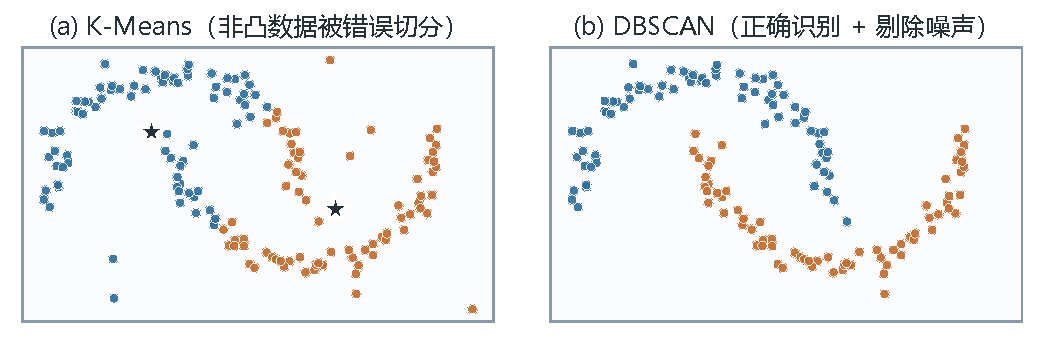
\includegraphics[width=0.92\textwidth]{pic/聚类效果对比示意图.pdf}
    \caption{聚类效果对比示意图}
    \label{fig:聚类效果对比示意图}
  \end{figure}

综合两种算法的特性可以看出，障碍物点云通常呈现任意形状、且不可预知簇数量、并伴随传感器噪声，这与DBSCAN算法所擅长处理的场景高度契合：它既无需预设障碍物数量，又能将离群噪声点自动剔除。因此，本章后续的点云检测器选用DBSCAN算法作为聚类内核，其检测流程将在下一节的障碍物检测跟踪系统中详细展开。

\section{障碍物检测跟踪系统}
受传感器配置与机载算力限制，移动机器人需要兼顾检测精度与计算效率。为此，本章构建如图~\ref{fig:障碍物检测与跟踪框架}所示的轻量级检测跟踪框架，主要包括障碍物检测、动态识别、状态跟踪和局部地图更新四个模块。

检测模块根据实际传感器配置接收深度图像或激光雷达点云。输入深度图像时，U深度图检测器直接从图像中提取障碍物，同时将深度图转换为点云并送入DBSCAN检测器；输入激光雷达点云时，则在裁剪与滤波后直接执行DBSCAN聚类。两个检测器输出的障碍物包围盒经过关联与融合后，由识别模块结合历史状态划分为静态目标和动态目标；跟踪模块完成跨帧数据关联并估计障碍物的运动状态；最后，地图更新模块将融合点云、障碍物边界及跟踪结果写入局部占用地图，为下游规划器提供环境约束。

\begin{figure}[!htb]
	\centering
	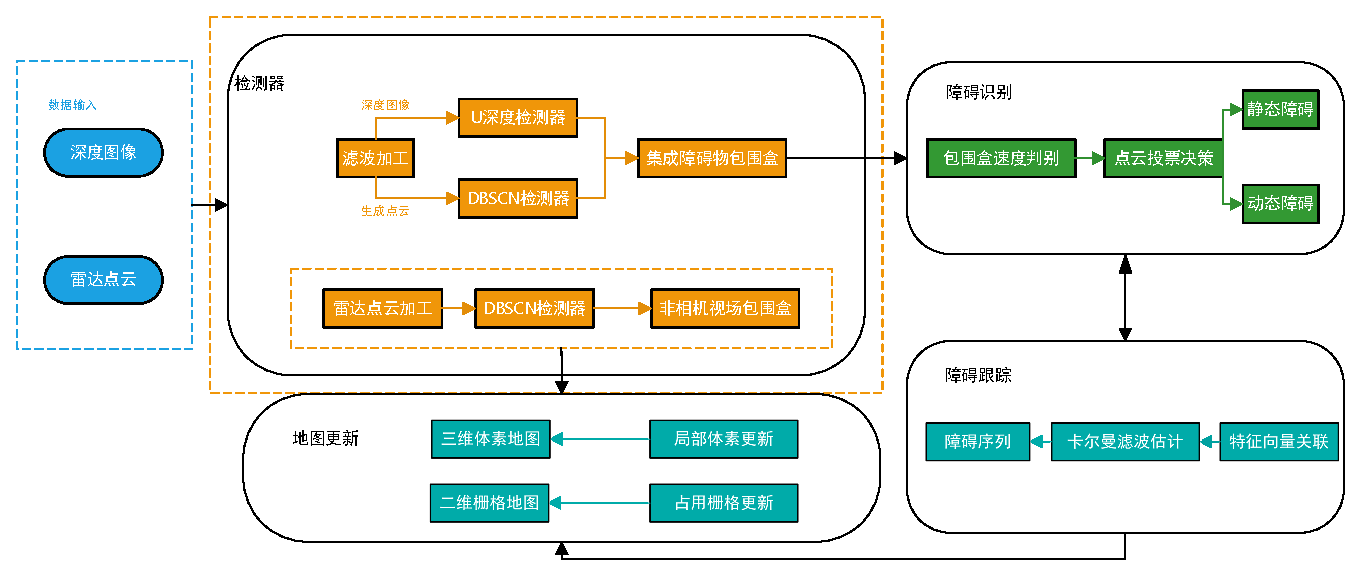
\includegraphics[width=\textwidth]{pic/检测流程.eps}
	\caption{障碍物检测与跟踪框架}
	\label{fig:障碍物检测与跟踪框架}
\end{figure}


\subsection{三维障碍物检测器}
环境检测由U深度图检测器与DBSCAN检测器组成。二者均采用非学习式方法，无需配置高算力推理硬件，适合部署于中小型移动机器人。U深度图检测器直接处理深度图像，DBSCAN检测器则处理由深度图反投影或由激光雷达获取的点云，两者对传感器噪声的敏感方式不同，可通过结果融合提高检测稳定性。

\textbf{（1）U深度图检测器。}U深度图方法已用于杂乱动态环境中的微型无人机避障\textsuperscript{\cite{7138979}}和拥挤室内环境中的动态目标检测\textsuperscript{\cite{10323166}}。该检测器通过三个步骤提取障碍物的三维轴对齐包围盒：生成U深度图、在U深度图中执行线段分组，以及在原始深度图中进行深度连续性搜索。

图~\ref{fig:检测器检测示意图}（a）和图~\ref{fig:检测器检测示意图}（b）分别为原始深度图像和U深度图像。系统按图像列统计深度值直方图生成U深度图，其横轴与原深度图像的列方向一致，纵轴表示离散深度区间。对U深度图中的连续区域进行分组，可得到图~\ref{fig:检测器检测示意图}（d）所示宽度为$w$、深度方向厚度为$t$的二维边界框；随后在原始深度图的对应列范围内执行深度连续性搜索，获得图~\ref{fig:检测器检测示意图}（a）所示的障碍物高度$h$。结合相机内参和深度值，即可将图像边界反投影至相机坐标系，再通过TF变换获得地图坐标系下障碍物的位置与三维尺寸。
\begin{figure}[!htb]
	\centering
	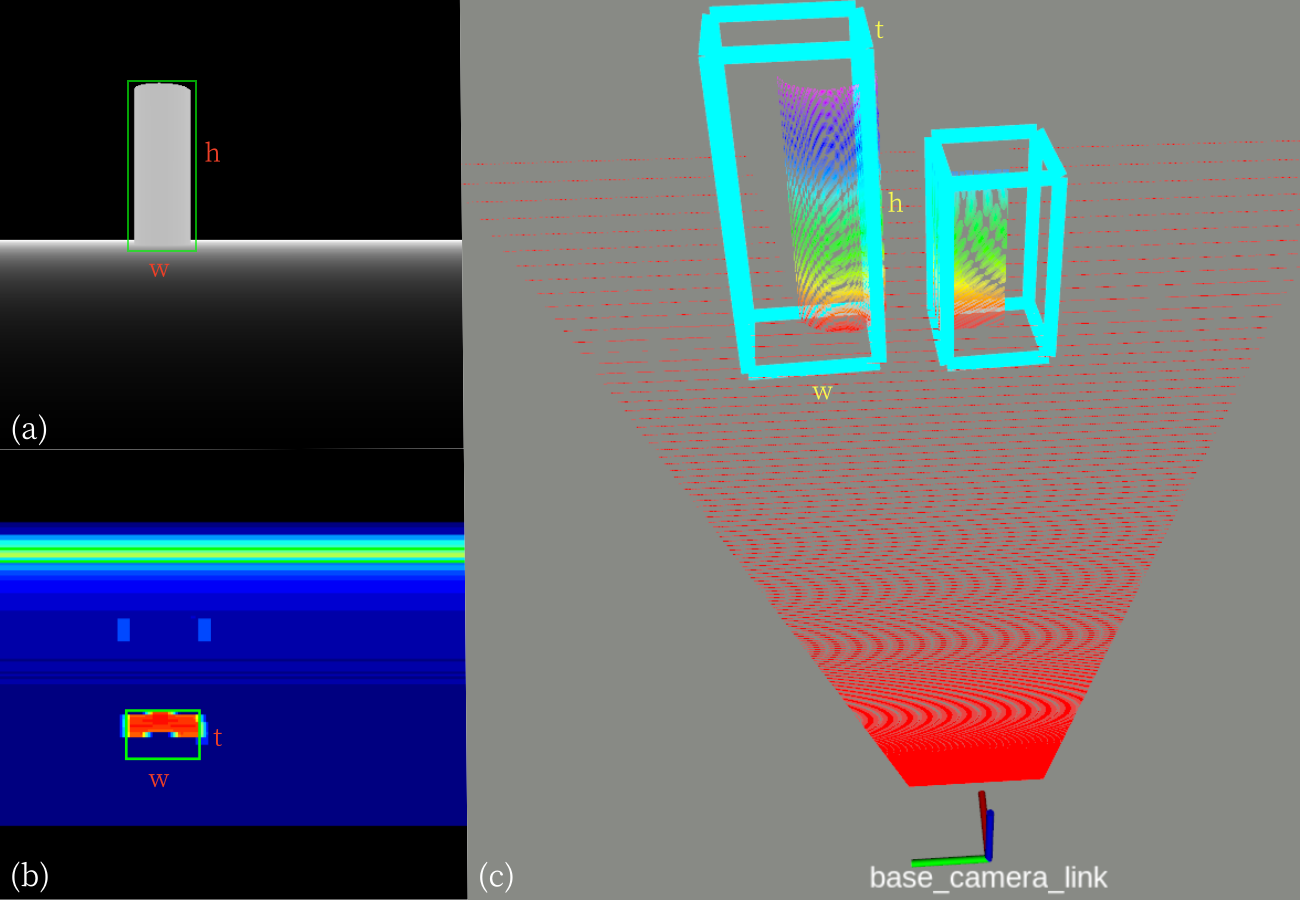
\includegraphics[width=0.85\textwidth]{pic/检测器检测示意图.png}
	\caption{检测器检测示意图}
	\label{fig:检测器检测示意图}
\end{figure}

\textbf{（2）DBSCAN检测器。}与基于图像的检测器不同，DBSCAN检测器直接处理点云数据。输入深度图像时，系统按第~\ref{sec:depth2cloud}节的方法将有效深度像素反投影为空间点；输入激光雷达点云时，则直接执行感兴趣区域裁剪。点云首先经过体素降采样和离群点过滤，再按第~\ref{sec:clustering}节所述DBSCAN方法聚类。对每个有效点簇分别计算最小、最大坐标，即可获得图~\ref{fig:检测器检测示意图}（c）所示的轴对齐包围盒。该检测器无需训练数据，且计算开销相对较低。

两个检测器并行运行并分别输出障碍物包围盒。由于深度图直方图与三维点云聚类具有不同的误差来源，同一真实障碍物通常会在两路结果中形成空间重叠，而单路噪声产生的伪检测往往缺少另一检测器的支持。因此，本文通过双向交并比（Intersection over Union, IoU）校验寻找两类结果中的一致检测，并采用保守策略融合相匹配的包围盒，以降低噪声对目标位置与尺寸估计的影响。

算法~\ref{alg:集成检测算法}给出了成对融合流程。对于检测器1输出的每个包围盒$b_{d1}$，先在检测器2的序列$B_{d2}$中搜索IoU最大的候选$b_{match1}$，再由$b_{match1}$反向搜索$B_{d1}$中的最佳匹配$b_{match2}$。仅当$b_{match2}=b_{d1}$且双向IoU均不低于阈值$S_{thr}$时，才将两者判定为互为最佳匹配。融合包围盒的中心取两者中心的平均值，各方向尺寸取两者对应尺寸的较大值，以避免低估障碍物范围。对于未通过匹配校验的检测结果，系统保留其原始包围盒，由后续跨帧跟踪进一步判断其有效性。

\begin{algorithm}[H]
    \KwIn{检测器1障碍物包围盒序列$B_{d1}$，检测器2障碍物包围盒序列$B_{d2}$，最小交并比阈值$S_{thr}$}
    \KwOut{集成包围盒序列$B_{en}$} 
    初始化$B_{en} \gets \emptyset$\;
    
    \For{$b_{d1} \in B_{d1}$}{
        $S_{iou1}, b_{match1} \gets \text{findBestIOUMatch}(b_{d1}, B_{d2})$\tcp{找到最佳匹配盒} 
        $S_{iou2}, b_{match2} \gets \text{findBestIOUMatch}(b_{match1}, B_{d1})$\tcp{反向验证匹配} 
        $flag \gets  (b_{match2} == b_{d1})$\; 
        
        \eIf{
            $S_{iou1} \geq S_{thr} \, \text{\normalfont\bfseries and} \, S_{iou2} \geq S_{thr} \, \text{\normalfont\bfseries and} \, flag$
        }{
            $b_{en} \gets \text{fuseBoxes}(b_{d1}, b_{match1})$\tcp{融合包围盒}
            $B_{en} \gets B_{en} \cup \{ b_{en} \}$\; 
        }{
            $B_{en} \gets B_{en} \cup \{ b_{d1} \}$\tcp{保留独立检测结果}
        }
    }
    返回$B_{en}$\;
    \caption{集成检测算法}
    \label{alg:集成检测算法}
\end{algorithm}

\subsection{障碍物关联跟踪}
当前帧检测得到的障碍物包围盒需与历史轨迹进行关联，以建立连续的目标身份并估计运动状态。本文采用基于特征相似度的匈牙利算法完成全局一一匹配\textsuperscript{\cite{JCDL202503143}}。与仅使用包围盒中心距离相比，联合考虑目标位置、尺寸和点云分布能够降低相邻动静态目标之间的错误关联概率。

深度相机可能因图像丢帧、目标遮挡或目标暂时离开视场而产生短时漏检。如图~\ref{fig:动态障碍物遮挡示意图}所示，机器人在前一时刻检测到墙后运动目标并生成避障轨迹；当目标短暂离开视场后，若立即删除其历史状态，规划器可能沿原路径继续运动，并在目标再次出现时来不及完成避让。为此，本文保留暂时失配目标的轨迹，并利用恒加速度模型在设定的最大丢失帧数内传播其状态；若后续观测重新匹配，则以新观测校正预测状态，否则在超过保留时限后删除该轨迹。该机制用于补偿短时观测中断，但预测不确定性会随失配时间增加，因此不能无限期保留外推结果。
\begin{figure}[!htb]
	\centering
	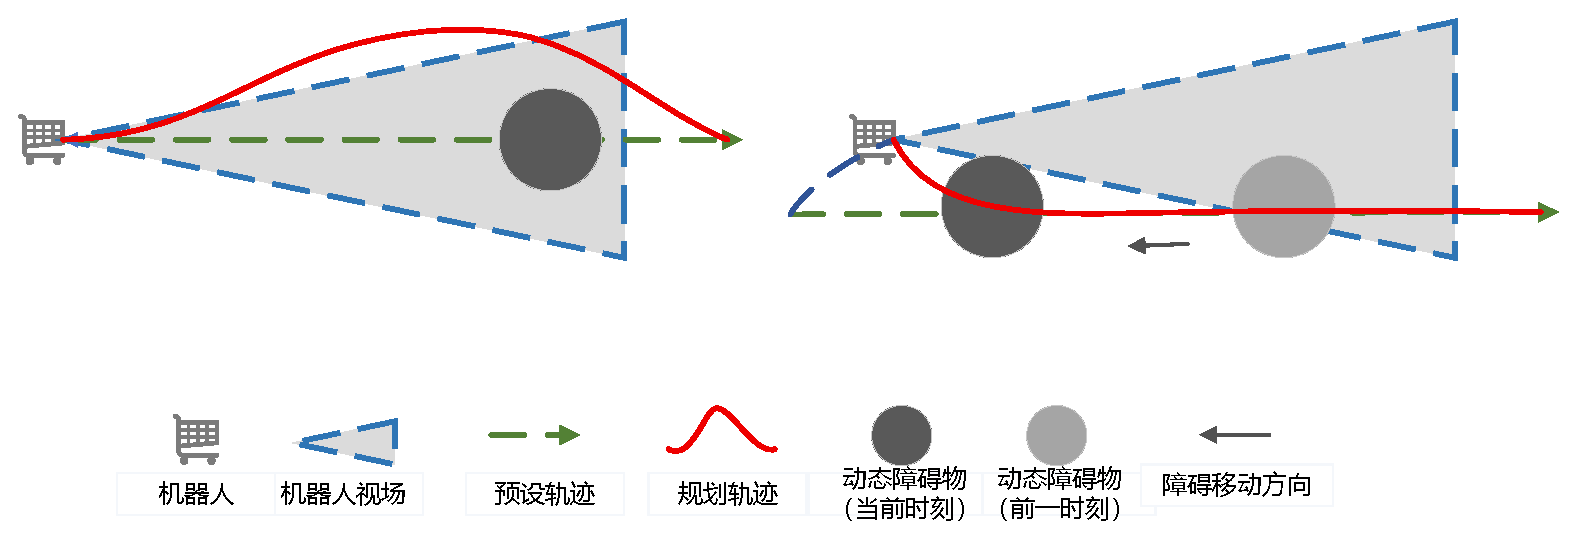
\includegraphics[width=1.0\textwidth]{pic/动态障碍物遮挡.eps}
	\caption{动态障碍物遮挡示意图}
	\label{fig:动态障碍物遮挡示意图}
\end{figure}

设第$i$个障碍物的归一化特征向量为
\begin{equation}
    \mathbf{f}(O_i)
    =\left[\mathbf{p}_i^{\mathrm{T}},\mathbf{d}_i^{\mathrm{T}},n_i,
    \boldsymbol{\sigma}_i^{\mathrm{T}}\right]^{\mathrm{T}},
    \label{eq:obstacle_feature}
\end{equation}
其中，$\mathbf{p}_i$为包围盒中心坐标，$\mathbf{d}_i$为包围盒在$x$、$y$、$z$方向上的尺寸，$n_i$为点簇所含点数，$\boldsymbol{\sigma}_i$为点簇坐标的标准差。各维特征按其统计尺度归一化后，定义障碍物$O_i$与$O_j$的相似度为
\begin{equation}
    s_{ij}
    =\exp\!\left(-\left\|\mathbf{f}(O_i)-\mathbf{f}(O_j)\right\|_2^2\right).
    \label{eq:obstacle_similarity}
\end{equation}
该函数将特征距离映射至$(0,1]$：距离越小，相似度越高。以$1-s_{ij}$构造关联代价矩阵，并通过匈牙利算法获得当前检测与历史轨迹之间的最小总代价匹配。为避免强制关联差异过大的目标，仅保留满足$s_{ij}\geq T_{sim}$的匹配对；未匹配检测用于初始化新轨迹，未匹配历史轨迹则进入短时预测保持状态。

障碍物完成数据关联后，采用二维恒加速度模型的卡尔曼滤波估计其运动状态。设地图坐标系下的状态向量为
\begin{equation}
    \mathbf{x}_t=[x_t,y_t,\dot{x}_t,\dot{y}_t,\ddot{x}_t,\ddot{y}_t]^{\mathrm{T}},
    \label{eq:ca_state}
\end{equation}
其中包含障碍物包围盒中心的二维位置、速度和加速度。采样间隔为$\Delta t$时，状态预测模型为
\begin{equation}
    \mathbf{x}_{t|t-1}=F\mathbf{x}_{t-1|t-1}+\mathbf{w}_t,
    \qquad \mathbf{w}_t\sim\mathcal{N}(\mathbf{0},Q),
    \label{eq:ca_prediction}
\end{equation}
其中
\begin{equation}
    F=\begin{bmatrix}
        1&0&\Delta t&0&\frac{1}{2}\Delta t^2&0\\
        0&1&0&\Delta t&0&\frac{1}{2}\Delta t^2\\
        0&0&1&0&\Delta t&0\\
        0&0&0&1&0&\Delta t\\
        0&0&0&0&1&0\\
        0&0&0&0&0&1
    \end{bmatrix}.
    \label{eq:ca_transition}
\end{equation}
若以零均值白噪声模拟模型未描述的平面加加速度，则可令$Q=GQ_jG^{\mathrm{T}}$，其中
\begin{equation}
    G=\begin{bmatrix}
        \Delta t^3/6&0\\0&\Delta t^3/6\\
        \Delta t^2/2&0\\0&\Delta t^2/2\\
        \Delta t&0\\0&\Delta t
    \end{bmatrix},\qquad Q_j=\sigma_j^2 I_2.
    \label{eq:ca_process_noise}
\end{equation}
参数$\sigma_j^2$表征真实目标运动偏离恒加速度假设的程度，其值越大，滤波器对新观测的响应越快，但状态估计的平滑性相应降低。

检测器直接观测的是包围盒中心位置，而非完整的六维运动状态。因此，观测模型写为
\begin{equation}
    \mathbf{z}_t=H\mathbf{x}_t+\mathbf{v}_t,
    \qquad \mathbf{v}_t\sim\mathcal{N}(\mathbf{0},R),
    \label{eq:ca_observation}
\end{equation}
\begin{equation}
    H=\begin{bmatrix}1&0&0&0&0&0\\0&1&0&0&0&0\end{bmatrix},
    \label{eq:ca_observation_matrix}
\end{equation}
其中，$R$为包围盒中心测量噪声协方差。卡尔曼滤波通过上述预测模型外推目标状态，并在获得新检测时利用位置观测完成校正；目标短时漏检时仅执行预测步骤，从而为视距外补偿提供连续的位置、速度与加速度估计。

\subsection{动态障碍物识别}
单独依据包围盒中心速度判断目标是否运动，容易将视场变化、包围盒尺寸抖动和关联误差造成的假位移误判为真实运动。为降低假阳性，本文采用“包围盒速度初筛—点云运动一致性复核”的两阶段判据：仅当包围盒中心速度超过阈值，且包围盒内足够比例的有效点与包围盒具有一致运动趋势时，才将目标标记为动态。对于连续多个历史帧均被判为动态的目标，采用有限时长的状态保持以避免短时漏检引起标签频繁切换。算法~\ref{alg:fusion1}给出了具体流程。

\begin{algorithm}[H]
	\caption{动态障碍物检测分类算法}
	\label{alg:fusion1}
	\SetAlgoLined
	\SetKw{Continue}{continue}
	\LinesNumbered
	\KwIn{目标障碍物列表$B_{tar}$，障碍物历史包围盒信息$BoxHist$，障碍物历史点云序列$PcHist$，强制执行帧数$forceFrame$，包围盒速度阈值$vbox_{th}$，点云速度阈值$vpc_{th}$，投票比例阈值$vote_{th}$}
    \KwOut{动态障碍物列表 $B_{dy}$} 
	
	\BlankLine
	$B_{dy} \leftarrow \emptyset$\;
	\For{$i \gets 0$ \KwTo $|B_{tar}|-1$} {
		$\texttt{DataAssociation}(B_{tar}[i], BoxHist)$ \tcp{关联当前包围盒与历史数据}
		$n \leftarrow |BoxHist[i]|$ \tcp{获取历史列表长度}
		\If{$\sum_{j=1}^{n} BoxHist[i][j].{is\_dynamic} \geq {forceFrame}$} 
		{
			$BoxHist[i][0].{is\_dynamic} \leftarrow {true}$\;
			$B_{dy}.{push\_back}(B_{tar}[i])$\tcp{添加到动态障碍物列表}
			\Continue\;	
		}
		${votes} \leftarrow 0$，$n_{valid}\leftarrow0$\tcp{初始化投票数与有效点数}
		$\mathbf{v}_{box}\leftarrow \left(\mathbf{P}_{box}(t)-\mathbf{P}_{box}(t-1)\right)/\Delta t$\;
		\ForEach{$p \in PcHist[i][0]$}{
			\If{$p$在$t-1$时刻存在有效对应点}{
				$n_{valid}\leftarrow n_{valid}+1$\;
				计算点速度$\mathbf{v}_{p}$\;
				\If{$\mathbf{v}_{p}^{\mathrm T}\mathbf{v}_{box}\geq0\;\&\&\;\|\mathbf{v}_{p}\|_2>vpc_{th}$}{
					$votes\leftarrow votes+1$\;
				}
			}
		}
		$r_{vote}\leftarrow votes/\max(n_{valid},1)$\;
		\If{$\|\mathbf{v}_{box}\|_2\geq vbox_{th}\;\&\&\;r_{vote}\geq vote_{th}$}{
			$B_{dy}.{push\_back}(B_{tar}[i])$\tcp{添加到动态障碍物列表}
		}
	}	
	返回$B_{dy}$\;
\end{algorithm}

算法首先将当前帧障碍物与历史轨迹关联，并检查对应轨迹的动态标签历史。若目标已连续多帧被判为动态，则在有限保持帧数内延续动态标签，以降低短时停顿或漏检造成的标签抖动。该滞回机制会延迟“运动转静止”的判定，因此保持帧数不宜过大。

对未触发标签保持的目标，包围盒中心速度由
\begin{equation}
    \mathbf{v}_{box}(t)
    =\frac{\mathbf{P}_{box}(t)-\mathbf{P}_{box}(t-1)}{\Delta t}
    \label{eq:bbox_velocity}
\end{equation}
计算。随后通过最近邻搜索建立当前点云与前一时刻点云之间的对应关系，并计算有效点速度$\mathbf{v}_p$。当$\mathbf{v}_p^{\mathrm T}\mathbf{v}_{box}\geq0$且$\|\mathbf{v}_p\|_2>vpc_{th}$时，该点为动态假设投一票。记有效对应点数为$n_{valid}$，则投票比例为$r_{vote}=votes/\max(n_{valid},1)$。仅当$\|\mathbf{v}_{box}\|_2\geq vbox_{th}$且$r_{vote}\geq vote_{th}$时，目标才被判为动态。

点云投票前还需剔除不具有跨帧对应关系的点。如图~\ref{fig:去除无效点云示意图}所示，机器人接近部分可见的静态障碍物时，视场扩大可能使包围盒中心由红色五角星位置移动至绿色五角星位置，从而产生较大的表观中心速度。当前帧中新出现的绿色点在前一帧不可见，无法形成可靠的速度观测；若将其计入投票，静态障碍物可能被误判为动态。因此，算法仅对两帧中均可见且匹配有效的点计算速度，并将新进入视场的点排除在投票集合之外。

\begin{figure}[!htb]
	\centering
	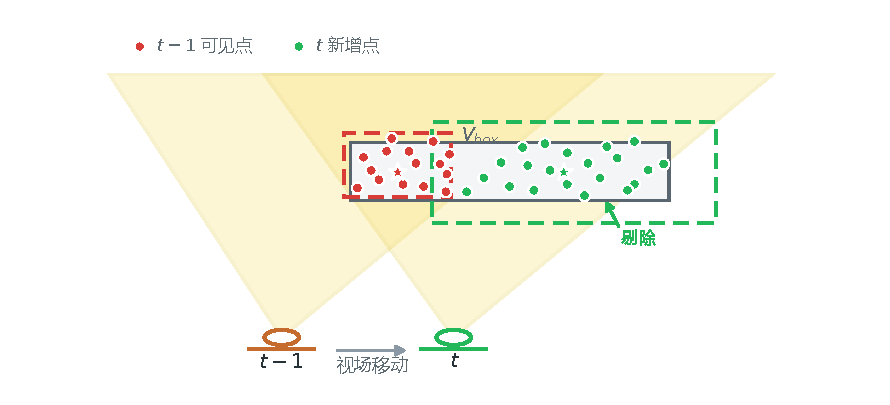
\includegraphics[width=1.0\textwidth]{pic/去除无效点云示意图.pdf}
	\caption{去除无效点云示意图}
	\label{fig:去除无效点云示意图}
\end{figure}

\section{局部地图构建策略}
本节与第2章的传感器级点云融合承担不同功能：第2章将激光雷达与深度相机观测统一到$\mathrm{base\_link}$坐标系，并发布去噪后的融合点云$\mathrm{/local\_pointcloud}$；本节以该点云以及障碍物检测、关联跟踪和动态状态识别结果为输入，构造直接服务于规划安全约束的局部占用地图。

系统首先结合同步位姿，将融合点云中的有效障碍点和包围盒边界点变换至地图坐标系；随后通过射线更新记录已观测自由空间与障碍占用，并在占用层上执行安全膨胀。输入观测与定位信息采用近似时间同步，以减小机器人运动造成的时空错位。为适应动态或半静态环境，系统同时维护局部更新窗口，使暂态误检和长期未被观测确认的陈旧占用能够被后续自由空间观测清除。

对于每个有效量测点，构造从传感器光心到量测端点的射线，并采用Bresenham算法\textsuperscript{\cite{9702849}}遍历射线覆盖的栅格单元。射线沿途单元记为自由，终端单元记为占用。设栅格$v$在时刻$t$的占用概率为$p_t(v)$，其对数几率表示为
\begin{equation}
    L_t(v)=\log\frac{p_t(v)}{1-p_t(v)}.
    \label{eq:local_map_logodds}
\end{equation}
使用对数几率后，多帧观测可通过增量累加完成融合。令自由观测增量$l_{free}<0$，占用命中增量$l_{occ}>0$，则栅格状态递推为
\begin{equation}
    L_t(v)=\operatorname{clip}\!\left(L_{t-1}(v)+\Delta L(v),L_{\min},L_{\max}\right),
    \label{eq:local_map_update}
\end{equation}
其中
\begin{equation}
    \Delta L(v)=
    \begin{cases}
        l_{free}, & v\in R_f,\\
        l_{occ},  & v=R_{end}.
    \end{cases}
    \label{eq:local_map_inverse_sensor}
\end{equation}
式中，$\operatorname{clip}(\cdot)$将对数几率限制在$[L_{\min},L_{\max}]$内，以避免重复观测造成数值饱和；$R_f$为射线沿途的自由栅格集合，$R_{end}$为射线终端栅格。连续自由观测可逐步降低陈旧占用的对数几率，从而释放已确认无障碍的空间。

为将机器人几何尺寸以及定位与控制误差纳入安全约束，系统在占用图上执行形态学膨胀。记阈值化后的占用集合为
\begin{equation}
    \mathcal{O}=\left\{v\mid p(v)>\tau\right\},
    \label{eq:occupied_set}
\end{equation}
其中$\tau$为占用概率阈值。设膨胀半径为$r_{infl}$，则膨胀后的障碍集合定义为
\begin{equation}
    \mathcal{O}^{\oplus}
    =\left\{u\mid \exists v\in\mathcal{O},\ \|u-v\|_2\leq r_{infl}\right\}.
    \label{eq:inflated_obstacle_set}
\end{equation}
实现中对新近更新的局部地图周期性执行膨胀，并生成布尔化的膨胀占用掩膜。由此，系统既保留障碍物边界信息，也记录视线内的自由空间证据，为下游路径规划提供可直接查询的安全约束。

\section{本章小结}
本章面向资源受限移动机器人在复杂动态环境中的障碍感知需求，研究了障碍物检测、关联跟踪、动态识别与局部地图更新方法。首先介绍K-Means和DBSCAN聚类原理，结合障碍物点云形状不规则、簇数量未知且含离群噪声的特点，选用DBSCAN作为点云检测器的聚类内核。

随后，构建了由U深度图检测器与DBSCAN点云检测器组成的轻量级并行检测框架，并通过双向IoU校验和保守包围盒融合降低单一检测器的误检影响。在跨帧跟踪阶段，采用归一化位置、尺寸和点云分布特征构造关联代价，通过匈牙利算法获得一一匹配；针对短时遮挡与目标暂时离开视场的情况，利用恒加速度卡尔曼滤波传播目标状态，为规划器提供连续的位置、速度与加速度估计。

在动态障碍物识别方面，采用包围盒中心速度进行初筛，并利用跨帧有效点的运动一致性进行投票复核；通过投票比例判据和有限时长的动态标签保持，降低包围盒抖动、视场变化和短时漏检引起的误判。最后，以第2章输出的多传感器融合点云及本章检测跟踪结果为输入，采用Bresenham射线遍历和对数几率更新记录自由空间与障碍占用，并通过形态学膨胀生成安全边界。

本章向第5章局部规划器提供三类信息：DBSCAN聚类后的障碍边界点及AABB包围盒，动态障碍物的位置、速度与加速度估计，以及包含自由空间和安全膨胀结果的局部占用地图。这些输出为动态预测点流构造和神经距离编码MPC的点级几何约束提供了环境输入。


\chapter{基于FAST\_LIO2的激光里程计定位算法研究}
\section{实时定位与地图构建（SLAM）}
实时定位与地图构建（Simultaneous Localization and Mapping）是移动机器人与自动驾驶领域的核心技术。其核心任务可归结为一种耦合估计问题：
在未知环境中，移动平台利用传感器数据，同步完成对自身运动状态的描述与对环境空间结构的建模。二者相互依赖，定位精度依赖于地图的准确性，
而一致地图的构建又需以精确的位姿轨迹为前提。
\section{SLAM方法架构及技术分类}
实时定位与地图构建作为一个复杂的状态估计问题，其解决方案已形成相对统一的系统架构。一个完整的SLAM系统通常包含以下几个关键模块：
前端里程计、后端优化、建图模块以及回环检测模块。传感器层面可分为激光雷达SLAM、视觉SLAM及多传感器融合SLAM，后端框架层面可分为基于滤波器的SLAM和基于图优化的SLAM。

前端里程计负责对相邻时刻的传感器数据进行关联与配准，实时估计传感器平台的增量运动，形成局部一致的轨迹与地图，
但其误差会随时间累积。后端优化则接收前端输出的位姿估计以及回环检测模块提供的非连续时刻的约束信息，构建一个以位姿为节点、以约束为边的概率图模型，
并通过非线性优化方法求解全局一致的最优轨迹。建图模块利用优化后的轨迹，将传感器观测数据融合到统一坐标系下，生成环境地图。
根据核心框架与传感器类型的不同，SLAM技术可进行如下分类：从传感器层面，主要分为激光雷达SLAM、视觉SLAM以及多传感器融合SLAM；
从后端框架层面，则主要分为基于滤波器的SLAM与基于图优化的SLAM两大类。

\subsection{基于滤波器的SLAM}
基于滤波器的SLAM方法将系统的状态（包括机器人位姿与环境路标点）建模为一个随时间演进的概率分布。
其核心思想是采用递归的贝叶斯估计框架，在每一时刻，根据当前的控制输入和传感器观测，对系统状态的置信度（后验概率）进行更新。
最具代表性的方法是扩展卡尔曼滤波器（EKF-SLAM）及其改进算法。EKF-SLAM通过线性化非线性运动与观测模型，在状态向量的高斯分布假设下，进行均值和协方差的递推更新。
此类方法的优势在于能够提供状态的在线估计及其不确定性度量，且计算复杂度与路标数量相关。然而，其线性化误差可能导致滤波器发散，且通常假设数据关联是已知或准确的。
FastSLAM算法通过粒子滤波估计路径，结合EKF估计路标，部分克服了EKF-SLAM的局限性，但粒子退化问题依然存在。在计算资源受限、强调实时性的应用场景中，基于滤波器的轻量化变体（如迭代卡尔曼滤波）仍具有重要价值。

\subsection{基于图优化的SLAM}
基于图优化的SLAM是当前主流的高精度SLAM框架。该方法将SLAM问题转化为一个大规模非线性最小二乘优化问题。其模型是一个图结构：节点表示机器人不同时刻的位姿（有时也包括环境路标），边则表示位姿节点之间的空间约束。
边主要分为两种：一是由前端里程计产生的连续位姿间的约束（里程计边），二是由回环检测产生的非连续位姿间的约束（回环边）。当检测到回环时，相当于在图中添加了新的强约束，
从而能够有效校正累积的里程计漂移。优化目标是寻找一组最优的节点状态（位姿），使得图中所有边代表的预测观测与实际观测之间的误差平方和最小。常用的优化工具包括高斯-牛顿法、列文伯格-马夸尔特算法等。
与滤波器方法相比，图优化方法能更自然地融合回环约束，进行全局一致性优化，从而获得精度更高的轨迹和地图，但其通常作为后端批量或滑动窗口优化运行，对计算资源要求较高。g2o、GTSAM、Ceres Solver等开源库为图优化SLAM的实现提供了强大支撑。

\subsection{紧耦合激光-惯性SLAM}
紧耦合激光-惯性SLAM是当前实现高鲁棒性、高频率状态估计的主流方案，其核心在于对激光雷达与惯性测量单元（IMU）的数据进行深层次融合。IMU能够以数百赫兹的频率测量角速度和加速度，在短时间内积分可提供高频但快速发散的位姿预测。
激光雷达则提供低频但绝对精度较高的三维几何观测。紧耦合方法并非将二者独立处理后再进行结果融合，而是在一个统一的状态估计框架内，直接使用原始的激光雷达点云和IMU测量值，共同约束系统状态（通常包括位置、姿态、速度、传感器偏置等）。
具体而言，激光雷达的每一个或多个原始点都可以直接作为观测方程，与IMU预测的运动方程一起，构建一个状态估计问题。这种深度融合方式充分利用了IMU的高频动态信息来辅助激光雷达点云的运动畸变矫正和数据关联，同时利用激光雷达的精确观测来抑制IMU积分漂移。
以FAST-LIO系列为代表的算法，通过将紧耦合的激光-惯性里程计建模在迭代卡尔曼滤波框架下，实现了在剧烈运动场景中的鲁棒、实时、高精度状态估计，是紧耦合SLAM的典型代表\textsuperscript{\cite{Xu2021FASTLIO}}。

\section{FAST\_LIO2激光惯性里程计原理}
FAST\_LIO2是一类面向实时三维建图与定位的紧耦合激光惯性里程计方法，其核心思想是在误差状态迭代卡尔曼滤波框架内融合IMU传播模型与激光点云到局部地图的几何约束\textsuperscript{\cite{Xu2022FASTLIO2}}。与LOAM类方法先提取边缘点、平面点再进行特征匹配的流程不同\textsuperscript{\cite{Zhang2014LOAM}}，FAST\_LIO2取消了手工特征提取模块，直接使用降采样后的原始激光点与地图进行配准。这种直接法能够保留更多环境几何信息，降低算法对雷达扫描模式和特征阈值的依赖，因此更适合Livox MID360等非重复扫描或小型移动平台常用的三维激光雷达。

FAST\_LIO2的系统流程可概括为：首先，利用IMU高频测量对状态进行前向传播，并在传播过程中对一帧激光点云内部的运动畸变进行补偿；其次，将去畸变后的点云变换到世界坐标系，在增量地图中搜索近邻点并拟合局部平面；最后，根据点到局部平面的残差构造量测模型，通过迭代卡尔曼滤波更新位姿、速度、IMU偏置以及外参等状态。为保证实时性，FAST\_LIO2采用增量式$k$维树（ikd-Tree）维护点云地图，使地图能够在线支持点插入、删除、重平衡和近邻搜索，避免每一帧重新构建静态KD树带来的高计算开销\textsuperscript{\cite{Cai2021ikdTree}}。

\begin{figure}[htbp]
  \centering
  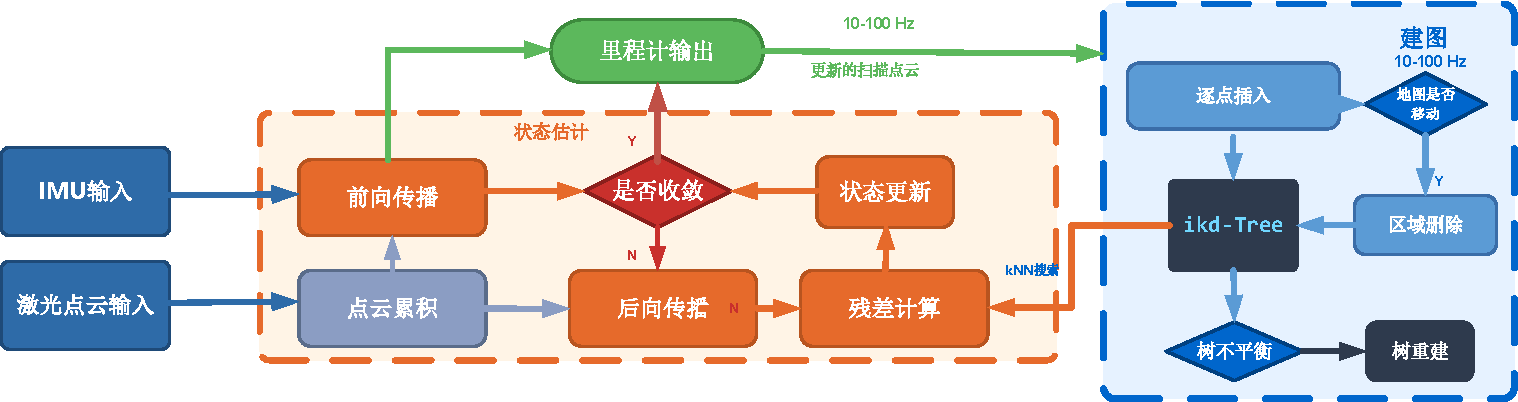
\includegraphics[width=\linewidth]{pic/激光惯性里程计系统架构.pdf}
  \caption{FAST-LIO2激光惯性里程计系统架构}
  \label{fig:fastlio_arch}
\end{figure}

系统由两大模块组成：
    （1）状态估计模块（橙色虚线框）：基于迭代误差状态卡尔曼滤波（IEKF），
    通过IMU前向传播、点云累积、后向传播、残差计算和状态更新的迭代循环，
    输出高频位姿估计；
   （2）建图模块（蓝色虚线框）：基于增量式kd树（ikd-Tree）维护局部点云地图，
    支持逐点插入、树上降采样、区域删除和动态重平衡，
    为状态估计提供kNN近邻搜索服务。
    输出的里程计位姿（绿色）既作为导航反馈，也驱动地图更新和前向传播的初值。

\subsection{状态变量与IMU传播模型}
图\ref{fig:fastlio_arch}展示了FAST\_LIO2的完整系统架构。其核心是状态估计与建图的紧密协同：IMU提供连续高频运动预测，激光雷达提供离散低频几何观测，二者在误差状态迭代卡尔曼滤波框架内深度融合。具体而言，系统在每帧同步数据到来时，首先利用IMU测量进行前向传播并补偿点云运动畸变；随后将去畸变点云累积并变换到世界坐标系，在ikd-Tree维护的增量地图中搜索近邻点，拟合局部平面并计算点到平面残差；最后通过迭代优化更新状态。当残差收敛时，输出当前位姿作为里程计结果并反馈至下一帧的前向传播初值；若未收敛，则继续后向传播进行下一轮迭代。建图模块根据输出位姿判断是否需要地图移动或区域删除，并将新观测点按体素分辨率插入ikd-Tree，保持地图的实时性与紧凑性。

设系统状态定义为
\begin{equation}
    \mathbf{x}
    =
    \left[
    {}^{G}\mathbf{p}_{I}^{T},
    {}^{G}\mathbf{R}_{I},
    {}^{I}\mathbf{R}_{L},
    {}^{I}\mathbf{p}_{L}^{T},
    {}^{G}\mathbf{v}_{I}^{T},
    \mathbf{b}_{g}^{T},
    \mathbf{b}_{a}^{T},
    {}^{G}\mathbf{g}^{T}
    \right],
    \label{eq:fastlio_state}
\end{equation}
其中${}^{G}\mathbf{p}_{I}$、${}^{G}\mathbf{R}_{I}$分别表示IMU坐标系相对于全局坐标系的位置和姿态，${}^{I}\mathbf{R}_{L}$、${}^{I}\mathbf{p}_{L}$表示激光雷达相对于IMU的外参，${}^{G}\mathbf{v}_{I}$为IMU速度，$\mathbf{b}_{g}$、$\mathbf{b}_{a}$分别为陀螺仪和加速度计偏置，${}^{G}\mathbf{g}$为重力向量。上述状态同时包含运动状态、传感器误差项和外参项，使激光几何约束能够与惯性传播约束在同一估计框架内共同作用。

IMU测量可表示为
\begin{equation}
    \boldsymbol{\omega}_{m}=\boldsymbol{\omega}+\mathbf{b}_{g}+\mathbf{n}_{g},
    \quad
    \mathbf{a}_{m}=\mathbf{a}+\mathbf{b}_{a}+\mathbf{n}_{a},
    \label{eq:imu_measurement}
\end{equation}
其中$\boldsymbol{\omega}_{m}$和$\mathbf{a}_{m}$为IMU输出的角速度和加速度，$\mathbf{n}_{g}$、$\mathbf{n}_{a}$为测量噪声。连续时间状态传播可写为
\begin{equation}
\begin{aligned}
    {}^{G}\dot{\mathbf{p}}_{I} &= {}^{G}\mathbf{v}_{I},\\
    {}^{G}\dot{\mathbf{R}}_{I} &= {}^{G}\mathbf{R}_{I}
    \left(\boldsymbol{\omega}_{m}-\mathbf{b}_{g}-\mathbf{n}_{g}\right)^{\wedge},\\
    {}^{G}\dot{\mathbf{v}}_{I} &= {}^{G}\mathbf{R}_{I}
    \left(\mathbf{a}_{m}-\mathbf{b}_{a}-\mathbf{n}_{a}\right)
    +{}^{G}\mathbf{g},\\
    \dot{\mathbf{b}}_{g} &= \mathbf{n}_{bg},\quad
    \dot{\mathbf{b}}_{a} = \mathbf{n}_{ba}.
\end{aligned}
    \label{eq:imu_propagation}
\end{equation}
式中$(\cdot)^{\wedge}$表示李代数向量到反对称矩阵的映射。由于激光雷达在采集一帧点云时平台仍在连续运动，若直接将整帧点云视为同一时刻采集，会在快速转弯或加减速时产生明显运动畸变。FAST\_LIO2利用IMU传播得到的连续位姿，对每个点按照其相对时间戳进行反向补偿，将其统一到该帧结束时刻，从而提升后续点云配准的一致性。

\subsection{直接点到地图量测模型}
在量测更新阶段，FAST\_LIO2将去畸变后的激光点${}^{L}\mathbf{p}_{j}$根据当前状态变换到全局坐标系：
\begin{equation}
    {}^{G}\mathbf{p}_{j}
    =
    {}^{G}\mathbf{R}_{I}
    \left(
    {}^{I}\mathbf{R}_{L}{}^{L}\mathbf{p}_{j}
    +{}^{I}\mathbf{p}_{L}
    \right)
    +{}^{G}\mathbf{p}_{I}.
    \label{eq:point_transform}
\end{equation}
随后在ikd-Tree维护的地图中搜索该点的若干近邻点，并利用近邻点拟合局部平面
\begin{equation}
    \mathbf{u}_{j}^{T}\mathbf{p}+d_{j}=0,
    \label{eq:local_plane}
\end{equation}
其中$\mathbf{u}_{j}$为平面单位法向量，$d_{j}$为平面参数。对应的点到平面残差为
\begin{equation}
    r_{j}
    =
    \mathbf{u}_{j}^{T}{}^{G}\mathbf{p}_{j}
    +d_{j}.
    \label{eq:point_plane_residual}
\end{equation}
该残差直接反映当前状态估计下激光点与局部地图几何的一致性。实际量测构造过程包括坐标变换、近邻搜索、局部平面估计、残差筛选和量测雅可比计算等步骤。当有效点数量不足或近邻无法稳定拟合平面时，系统应降低该帧几何约束的可信度，以避免退化环境对滤波器造成错误修正。

设一帧中所有有效点残差堆叠为$\mathbf{r}$，量测模型可近似写为
\begin{equation}
    \mathbf{0}
    =
    \mathbf{h}(\mathbf{x})+\mathbf{v},
    \quad
    \mathbf{h}(\mathbf{x})=
    \left[r_{1},r_{2},\cdots,r_{m}\right]^{T},
    \label{eq:fastlio_measurement}
\end{equation}
其中$m$为有效量测点数量，$\mathbf{v}$为激光量测噪声。由于位姿状态位于$SO(3)$流形上，FAST\_LIO2采用流形上的误差状态迭代卡尔曼滤波进行求解：先由IMU传播得到预测状态，再在当前线性化点附近反复构建点到平面残差和雅可比，迭代修正误差状态，直至收敛或达到最大迭代次数。与传统ICP单独输出刚体变换不同，该过程将点云几何约束直接融入包含IMU偏置、速度和外参的统一状态估计中，因此能够同时获得低延迟和较高鲁棒性。

\subsection{基于ikd-Tree的增量地图维护}
激光里程计需要在每帧点云到来时进行地图近邻搜索和地图更新。若每次都对全局点云重新构建KD树，计算复杂度会随着地图规模迅速上升，难以满足在线定位需求。FAST\_LIO2使用ikd-Tree维护局部稠密点云地图，该结构除支持近邻搜索外，还支持增量插入、按空间区域删除、树结构重平衡以及树上体素降采样。

如图\ref{fig:fastlio_arch}右侧建图模块所示，ikd-Tree不仅提供kNN近邻搜索服务，还需动态响应传感器移动和环境变化。当机器人移动导致地图边界发生偏移时（地图移动?判断为真），系统触发区域删除操作，移除视野外的历史点云以控制内存占用。插入新点时，ikd-Tree首先执行树上降采样（On-Tree Downsampling），判断新点是否能够补充地图几何信息：若该体素内已有代表点且新点不提供额外约束，则跳过插入；否则将其增量加入树结构。此外，频繁的插入和删除会导致树的不平衡，当不平衡度超过阈值时，系统触发局部或全局重平衡（树重建），恢复树的查询效率。该动态维护机制使FAST\_LIO2能够在长时间运行中保持稳定的计算开销。

本文采用的地图维护策略与FAST\_LIO2一致：系统首先将当前帧降采样点云变换到世界坐标系，再依据体素分辨率判断新观测是否能够补充地图几何信息。若某一体素内已经存在更具代表性的地图点，则当前点不再重复插入；若当前点能够提供新的空间约束，则将其作为增量点加入地图索引。对于预建地图定位任务，地图更新可以被关闭，使所有量测始终约束在固定的全局地图中；对于未知区域探索或地图扩展任务，则可在完成初始定位后开启增量更新，使新观测逐步并入原有地图。该策略使定位模式和建图扩展模式能够在同一状态估计框架下统一描述。

\section{面向预建地图的FAST\_LIO2定位与重定位方法}
原始FAST\_LIO2更侧重在线里程计与建图，其输出轨迹不可避免地存在长距离累积漂移。对于运维机器人在变电站、厂房或室内走廊等已知场景中的重复巡检任务，系统更需要在预先构建的全局点云地图中获得稳定、可复现的绝对位姿。因此，本文在FAST\_LIO2直接激光惯性里程计框架基础上，引入预建点云地图约束和有初值重定位机制，将在线里程计问题转化为地图坐标系下的连续位姿估计问题。该方法并非改变FAST\_LIO2的紧耦合状态估计本质，而是在滤波器量测更新阶段使用固定全局地图提供几何先验，从而抑制纯里程计运行中的坐标漂移。

本文所提出的定位框架如图\ref{fig:map_localization}所示，系统分为初始化（阶段A）和在线定位（阶段B）两个阶段。阶段A完成地图加载与ikd-Tree索引构建、IMU静态初始化以及近似初值与ICP相结合的两阶段初始对齐，为后续状态估计提供可靠的初始位姿；阶段B在每帧数据到来时执行IMU传播、点云去畸变、地图坐标变换、ikd-Tree近邻搜索与IEKF状态更新，持续输出地图坐标系下的全局连续位姿，并可根据任务需求在纯定位模式与混合建图模式之间切换。

\begin{figure}[htbp]
  \centering
  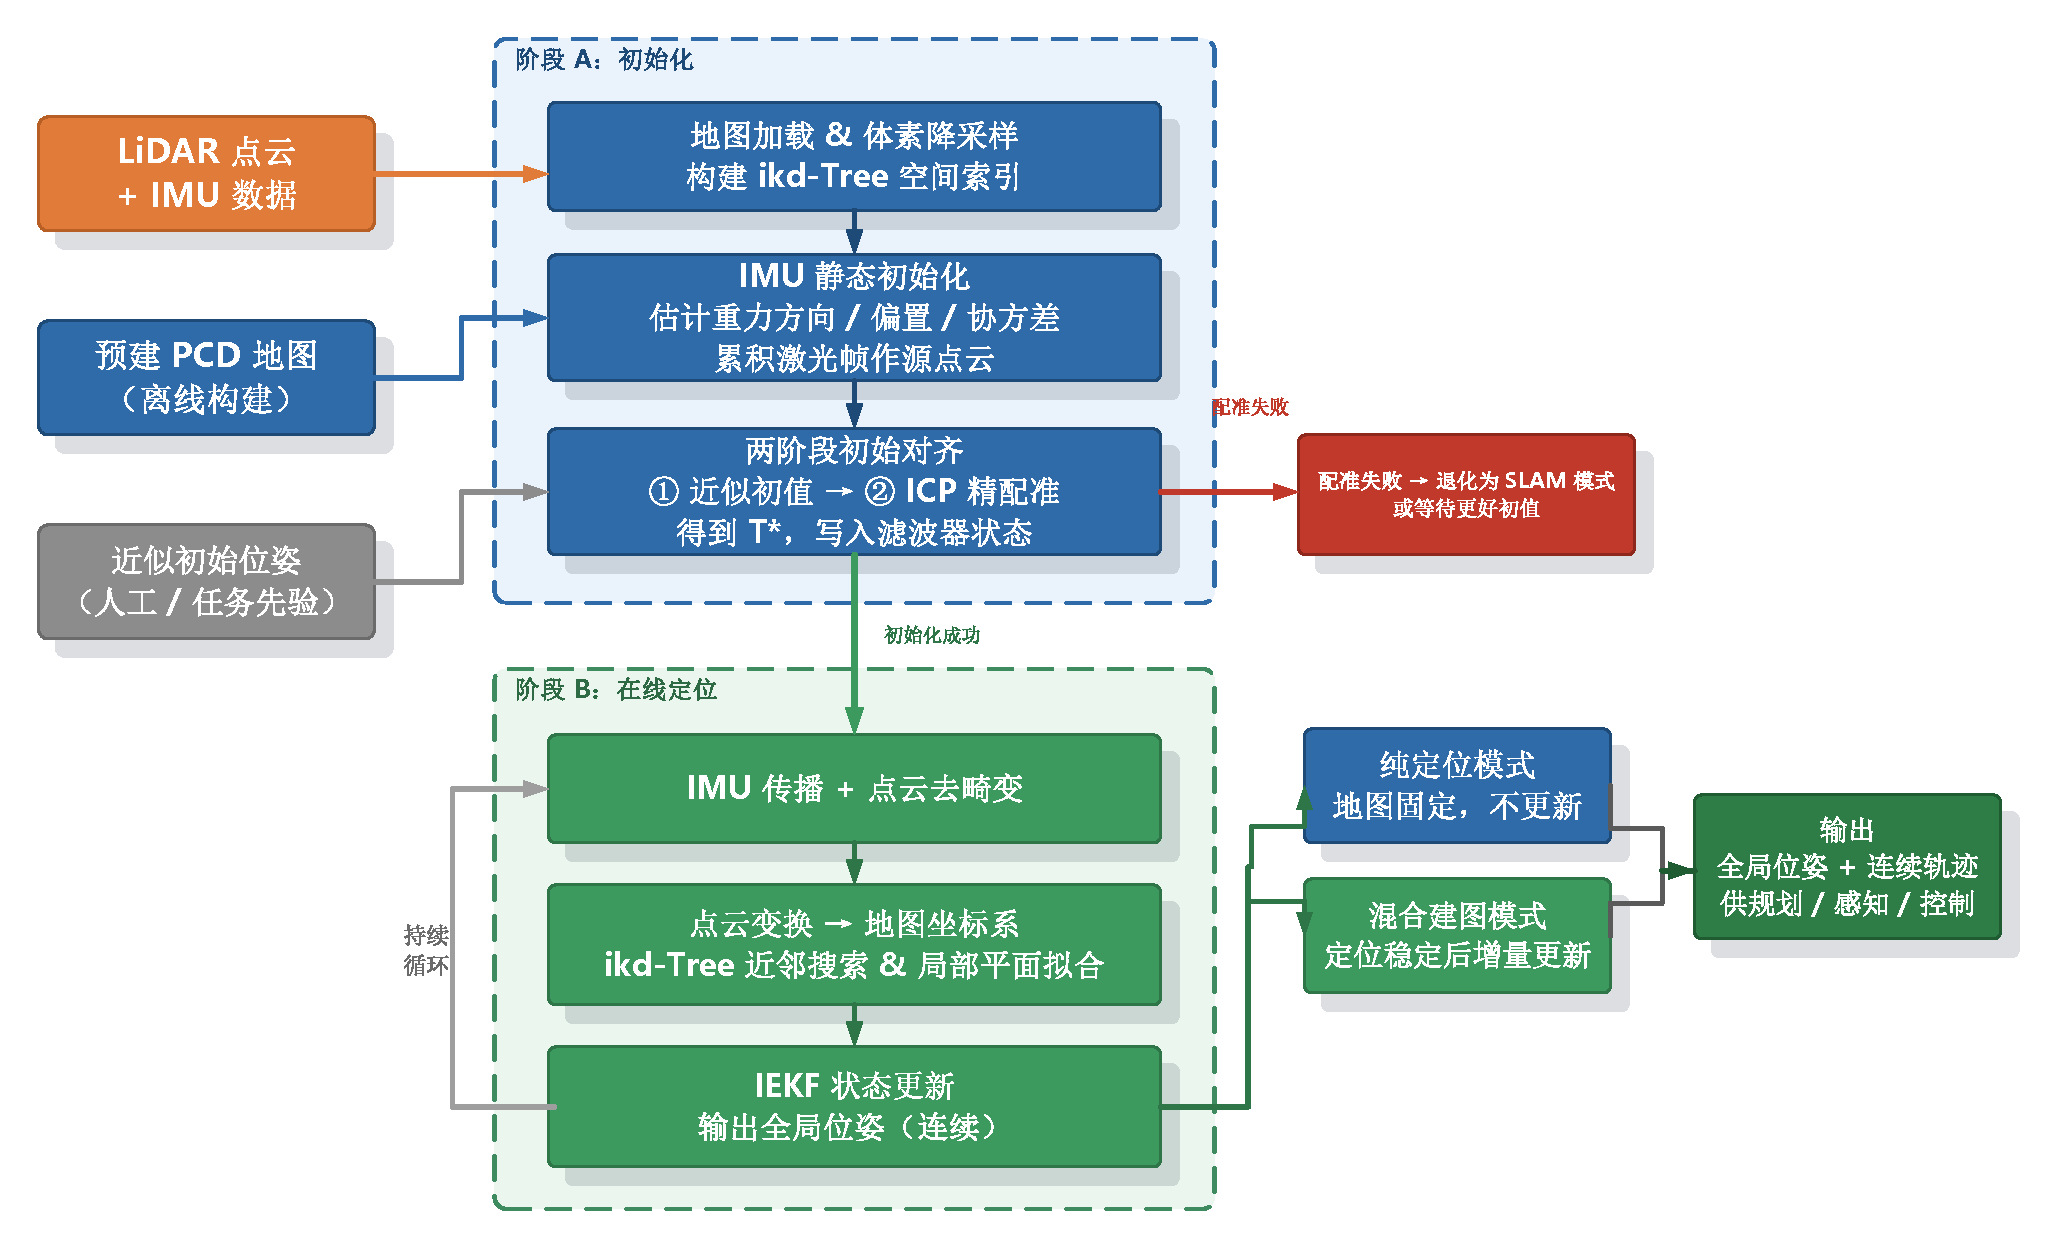
\includegraphics[width=0.92\linewidth]{pic/预建地图定位框架.pdf}
  \caption{基于预建地图的FAST-LIO2定位框架}
  \label{fig:map_localization}
\end{figure}

\subsection{预建地图定位框架}
预建地图定位系统的输入由三部分构成：一是连续到达的激光雷达点云和IMU测量，二是离线构建得到的全局点云地图，三是机器人在地图坐标系中的初始位姿近似。激光与惯性数据用于提供高频运动预测和局部几何观测，预建地图用于提供全局坐标基准，初始位姿近似则用于保证启动阶段点云配准能够收敛到正确邻域。

系统输出为地图坐标系下的机器人位姿、连续轨迹以及经位姿变换后的当前帧点云。对于上层路径规划和运动控制模块而言，该输出相当于全局定位反馈；对于感知和地图更新模块而言，该输出提供了将局部观测投影到统一坐标系的时变位姿。为了避免导航任务在定位尚未收敛前启动，系统在初始化完成前应保持任务锁定状态，待地图加载、IMU初始化和初始配准均满足条件后再向上层模块释放定位可用信号。

\subsection{预建地图加载与初始位姿对齐}
定位流程启动后，系统首先读取离线构建的PCD点云地图，并通过均匀采样或体素滤波降低冗余点密度。随后，以预建地图初始化增量式空间索引，使后续点云配准能够直接在全局地图中进行近邻搜索。完成该步骤后，地图不再只是里程计运行过程中逐步生成的局部几何集合，而是作为固定的全局几何先验参与后续每帧激光量测更新。

由于点云配准通常是局部优化问题，启动阶段需要较可靠的初始位姿。本文采用“近似初值 + ICP精配准”的两阶段初始化策略：首先由人工设定、停靠位置或上层先验给出机器人在预建地图中的粗略位姿；然后在IMU静态初始化完成后，累积若干帧激光点云形成局部源点云，并将其与预建地图进行ICP配准\textsuperscript{\cite{Besl1992ICP}}。ICP的目标可表示为
\begin{equation}
    \mathbf{T}^{*}
    =
    \arg\min_{\mathbf{T}\in SE(3)}
    \sum_{i}
    \left\|
    \mathbf{T}\mathbf{p}_{i}
    -
    \mathbf{q}_{\pi(i)}
    \right\|^{2},
    \label{eq:icp_init}
\end{equation}
其中$\mathbf{p}_{i}$为启动阶段累积的局部点云，$\mathbf{q}_{\pi(i)}$为预建地图中的对应点，$\mathbf{T}^{*}$为源点云到地图坐标系的最优刚体变换。ICP收敛后，得到的位姿修正被写入滤波器初始状态，使后续激光惯性状态估计直接在预建地图坐标系下展开。若初始配准无法收敛，则说明粗略位姿、当前观测或地图几何之间存在较大不一致，此时不应继续启动导航任务，以避免错误初值引起持续定位发散。

上述两阶段初始对齐过程如图\ref{fig:icp_align}所示。首先由近似初值将启动阶段累积的源点云$\mathbf{p}_{i}$粗略摆放到预建地图的正确邻域，此时源点云与地图之间仍存在明显的旋转和平移偏差（图\ref{fig:icp_align}(a)）；随后进入ICP迭代精配准，在每次迭代中先为源点建立到地图的最近邻对应$\mathbf{p}_{i}\leftrightarrow\mathbf{q}_{\pi(i)}$，再求解使式\eqref{eq:icp_init}最小的刚体变换并更新源点云位姿（图\ref{fig:icp_align}(b)），如此反复直至点对残差收敛至阈值$\varepsilon$；最终得到的最优变换$\mathbf{T}^{*}$将源点云精确对齐到地图坐标系（图\ref{fig:icp_align}(c)），并写入滤波器初始状态。其中点对残差是否收敛至阈值$\varepsilon$可作为初始化是否成功的判据，若残差无法收敛则放弃本次启动对齐。

\begin{figure}[htbp]
  \centering
  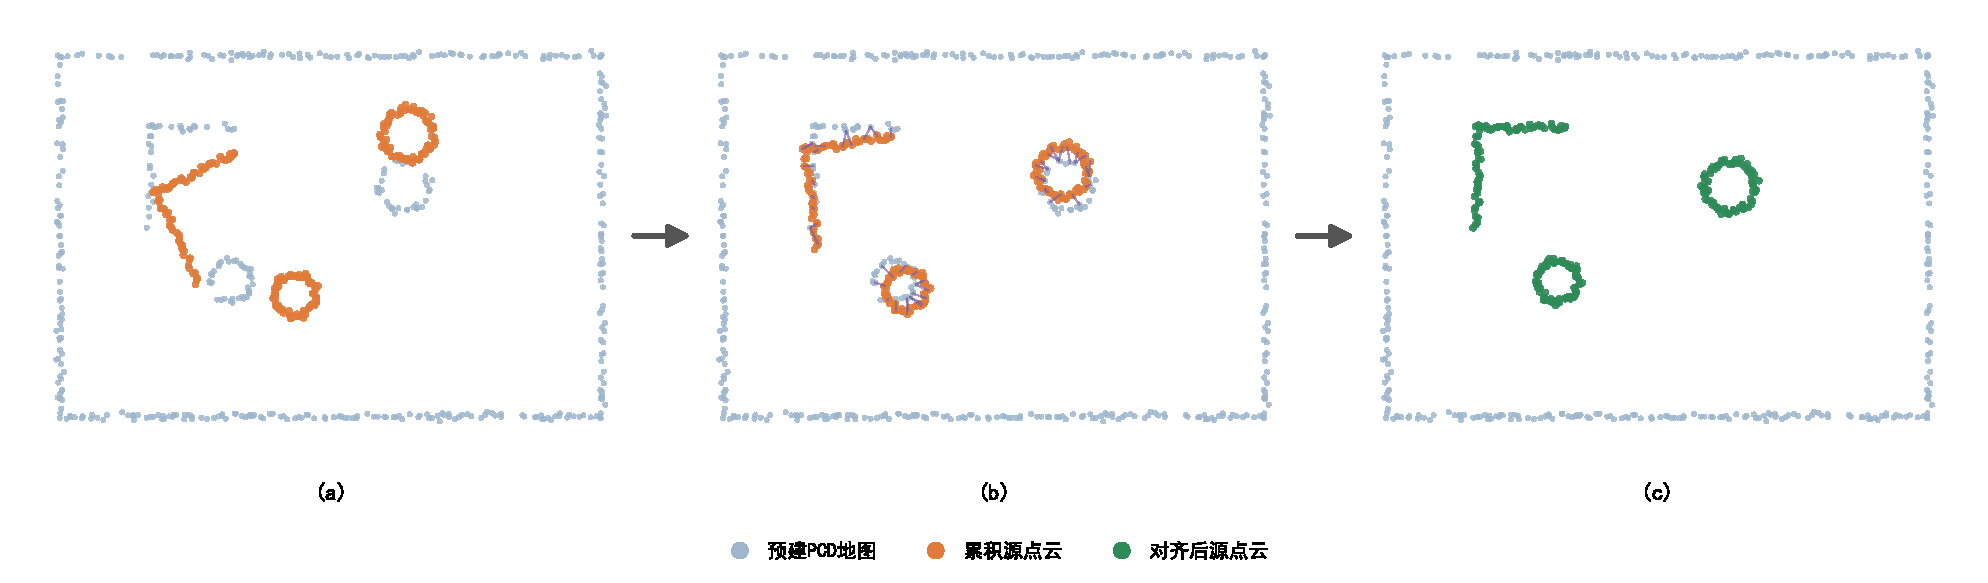
\includegraphics[width=\linewidth]{pic/两阶段ICP初始对齐.pdf}
  \caption{两阶段初始对齐过程示意}
  \label{fig:icp_align}
\end{figure}

\subsection{地图约束下的在线定位更新}
完成初始对齐后，系统进入逐帧定位阶段。每当激光点云与IMU数据完成时间同步，状态估计器首先根据IMU序列进行状态传播，并对当前帧点云进行运动畸变补偿；随后，将去畸变点云变换到地图坐标系，在预建地图中搜索近邻点并拟合局部平面，构造点到平面的残差；最后，通过迭代误差状态卡尔曼滤波更新机器人位姿、速度和IMU偏置。由于纯定位模式下地图保持固定，激光量测始终约束在同一全局地图坐标系内，输出位姿也自然具有全局一致性。

从算法结构看，该流程可抽象为以下步骤：

（1）加载预建点云地图，对地图点云进行降采样，并构建空间索引。

（2）利用启动阶段IMU数据估计重力方向、陀螺仪偏置和初始协方差，同时累积若干帧激光点云作为初始配准源点云。

（3）若预建地图有效，则以近似初值执行ICP配准，将得到的修正变换写入滤波器状态，并将定位状态标记为可用；若预建地图为空或点数不足，则退化为普通SLAM模式。

（4）在每一帧同步后的激光和IMU数据到来时，先进行IMU传播和点云去畸变，再将当前帧点云降采样并变换到地图坐标系。

（5）在地图索引中搜索近邻点并拟合局部平面，构造点到平面残差和量测雅可比，通过迭代卡尔曼滤波更新状态。若系统处于混合建图模式，则将满足条件的新观测增量并入地图。

\subsection{纯定位模式与混合建图模式}
根据地图是否随在线观测更新，本文方法可分为纯定位模式和混合建图模式。纯定位模式仅使用预建地图进行位姿估计，不将当前帧点云写入地图。这种模式适用于已经完成地图采集、巡检路线相对固定的场景，能够避免动态障碍物、临时设备或点云噪声污染全局地图。混合建图模式则在完成初始定位并稳定运行后允许地图增量更新，适用于预建地图不完整或机器人需要探索扩展区域的场景。此时新采集点云会在当前地图坐标系下并入地图，使扩展区域与原始地图保持同一坐标基准。

需要注意的是，本文所述重定位主要指系统启动或任务重启时基于近似初值的地图坐标恢复，而不是完全无先验的全局定位。由于ICP属于局部优化方法，初始位姿误差过大、环境几何重复、视场内有效结构过少或预建地图与当前环境差异过大时，配准可能收敛到错误局部最优。因此，在实际部署中应结合机器人停靠点、人工给定初值、二维码/定位桩、轮速里程计或上层任务先验提供合理初始位姿。同时，机器人应在地图加载和初始化期间保持静止，以保证IMU初始化和点云累积质量。

\section{本章算法特点与适用性分析}
相较于仅依赖轮式里程计或AMCL粒子滤波的二维定位方法，基于FAST\_LIO2的三维激光惯性定位具有以下优势。首先，三维点云能够直接利用墙面、设备支架、电缆沟边缘和立体障碍物等空间结构，在平面纹理不明显或二维激光可见特征不足时仍可提供较强约束。其次，IMU传播为高频状态估计和点云去畸变提供支撑，可提升机器人在转弯、加减速和短时遮挡条件下的定位连续性。再次，直接点到地图配准减少了特征提取阈值对不同雷达型号和扫描模式的依赖，有利于系统在不同传感器平台上的迁移。

该方法也存在一定局限。其一，FAST\_LIO2本质上仍是局部里程计框架，若脱离预建地图或回环后端，长距离运行会产生漂移；本文通过固定预建地图定位减轻该问题，但地图本身的质量会直接影响定位效果。其二，激光几何约束依赖足够丰富的空间结构，在长直走廊、开阔区域、单一大平面或近距离遮挡严重场景中可能出现退化。其三，该启动重定位策略依赖近似初值和ICP收敛性，不适合直接处理完全未知初始位置。针对上述问题，后续可进一步引入全局点云描述子、回环检测或多源传感器辅助定位，以提升全局重定位能力和长期运行稳定性。
\section{本章小结}
本章围绕移动机器人定位需求，研究了基于FAST\_LIO2的激光里程计定位算法。首先介绍了SLAM系统的基本架构和技术分类，分析了基于滤波器、基于图优化以及紧耦合激光惯性SLAM方法的特点。随后重点阐述FAST\_LIO2的核心原理，包括IMU状态传播、激光点云运动畸变补偿、直接点到地图残差、流形迭代卡尔曼滤波以及ikd-Tree增量地图维护机制。

在此基础上，本章说明了面向预建PCD地图的定位与启动重定位流程。系统通过加载预建地图构建空间索引，以近似初始位姿和ICP完成地图坐标系下的初始对齐，并在后续运行中利用FAST\_LIO2的点到平面量测更新持续输出全局位姿。通过区分纯定位模式和混合建图模式，所述方法能够在固定地图巡检和地图扩展两类任务之间切换，为后续路径规划、障碍物检测和导航控制模块提供稳定的位姿基础。


\chapter{实物平台实验验证}
\section{引言}
第5章在Gazebo仿真环境中建立了神经距离编码MPC与对比方法的统一实验协议。仿真环境的传感器噪声模型、障碍几何和底盘动力学均为理想化设定，无法反映真实激光雷达的量测稀疏与遮挡、定位漂移、通信延迟以及底盘执行偏差对局部规划的影响。因此，本章在自研移动机器人平台上开展实物实验，用于检验前述感知、定位与规划模块构成的导航软件链路在真实条件下能否稳定协同运行，并记录典型非凸障碍环境中的运行形态。

本章的证据定位与第5章不同：仿真实验承担不同方法在统一条件下的定量比较，实物实验承担真实平台上的部署可行性与运行稳定性验证，不复现仿真场景的完整统计对比。

\section{实验平台与运行环境}
实验采用自研移动机器人平台，搭载第2章所述Livox MID-360三维激光雷达，机载计算平台运行Ubuntu 20.04与ROS Noetic，实时定位由第3章基于FAST-LIO2与预建点云地图的定位模块提供，障碍检测与局部地图由第4章模块生成，局部规划控制频率为10\,Hz。该平台采用麦克纳姆轮全向底盘，与第5章仿真被控对象的运动学形式一致，实验中按式~\eqref{eq:ROS速度指令}的接口接收规划器输出的机体系两个平移速度分量与角速度，因此被控对象的实际运动与式~\eqref{eq:全向底盘离散运动模型}的建模假设保持一致。规划器所加载的距离编码器权重与仿真实验相同：编码器的输入输出仅由底盘轮廓尺寸决定，与仿真/实物的运行环境无关，因此无需为实物实验重新训练。

现有实物材料包含L型非凸障碍和多障碍组合两类环境。由于不同照片的障碍布局、机器人位置和拍摄范围并不完全一致，本章不将其排成“同一目标点下两种方法对比”或“连续导航过程”，而仅作为实验平台、典型障碍布局和运行状态的场景记录。

\begin{figure}[!htb]
	\centering
	\subfloat[L型非凸障碍场景]{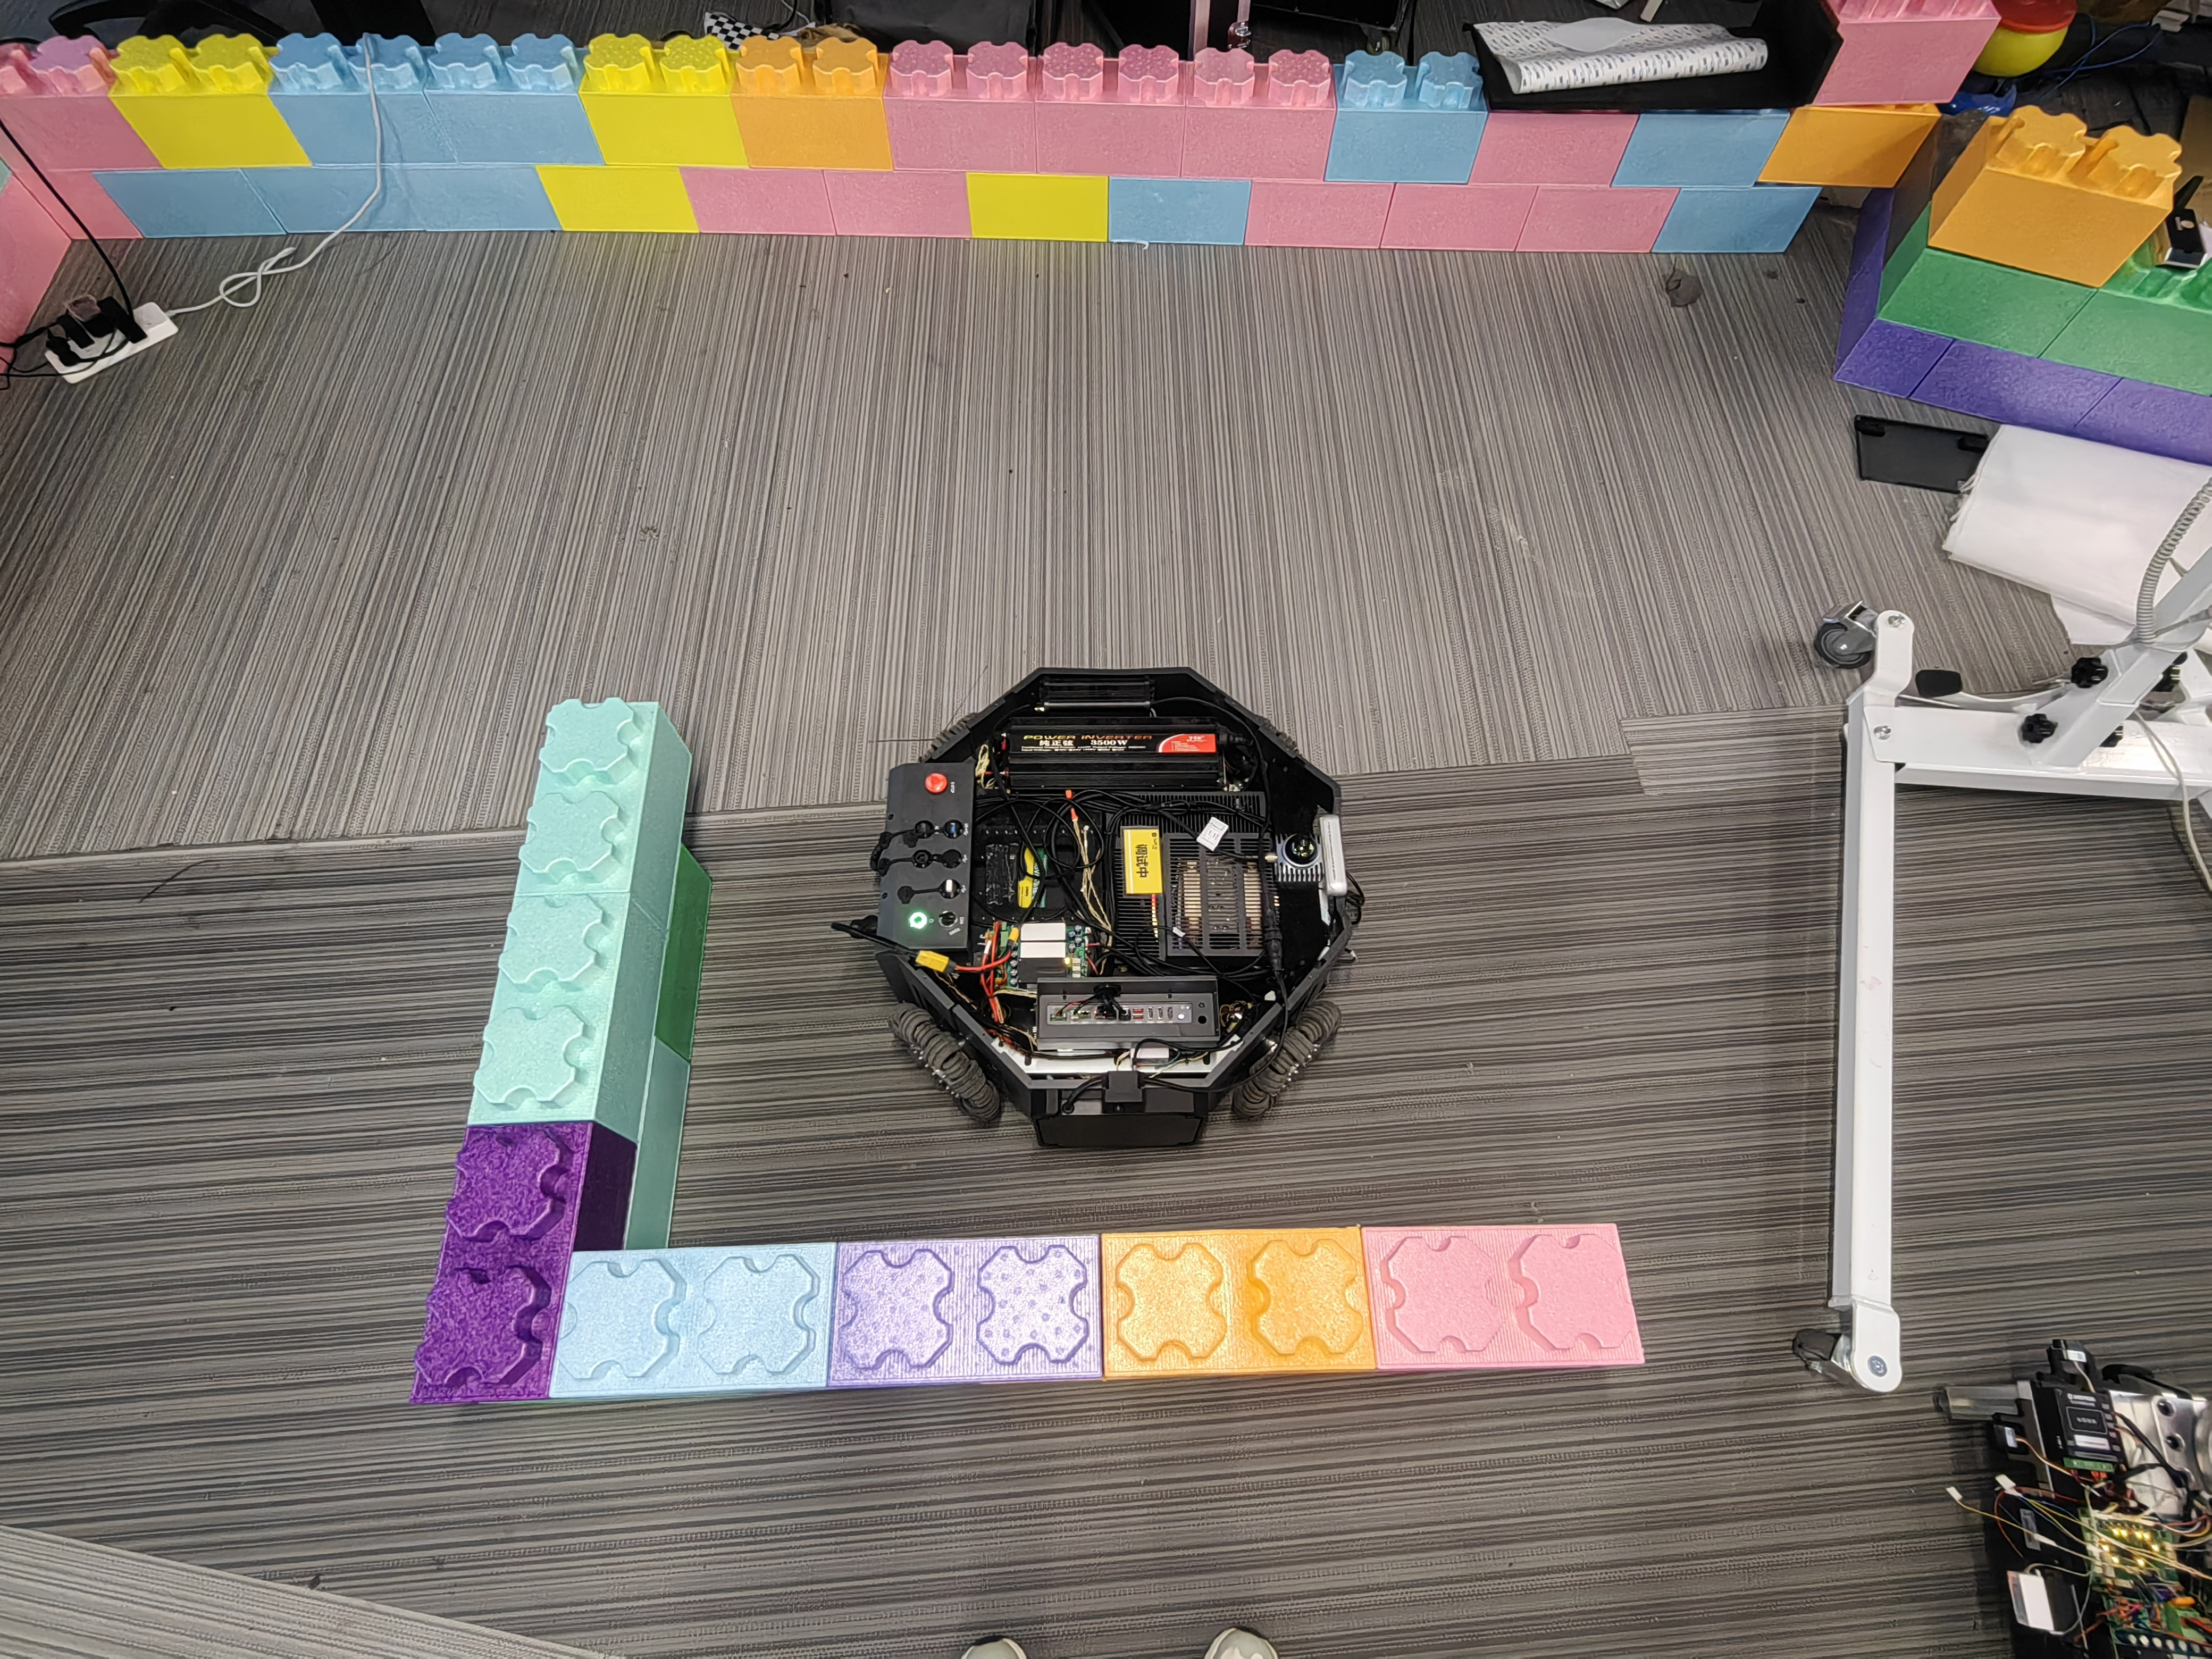
\includegraphics[width=0.48\textwidth]{pic/exp_goal1_neupan.jpg}}
	\hfill
	\subfloat[多障碍组合场景]{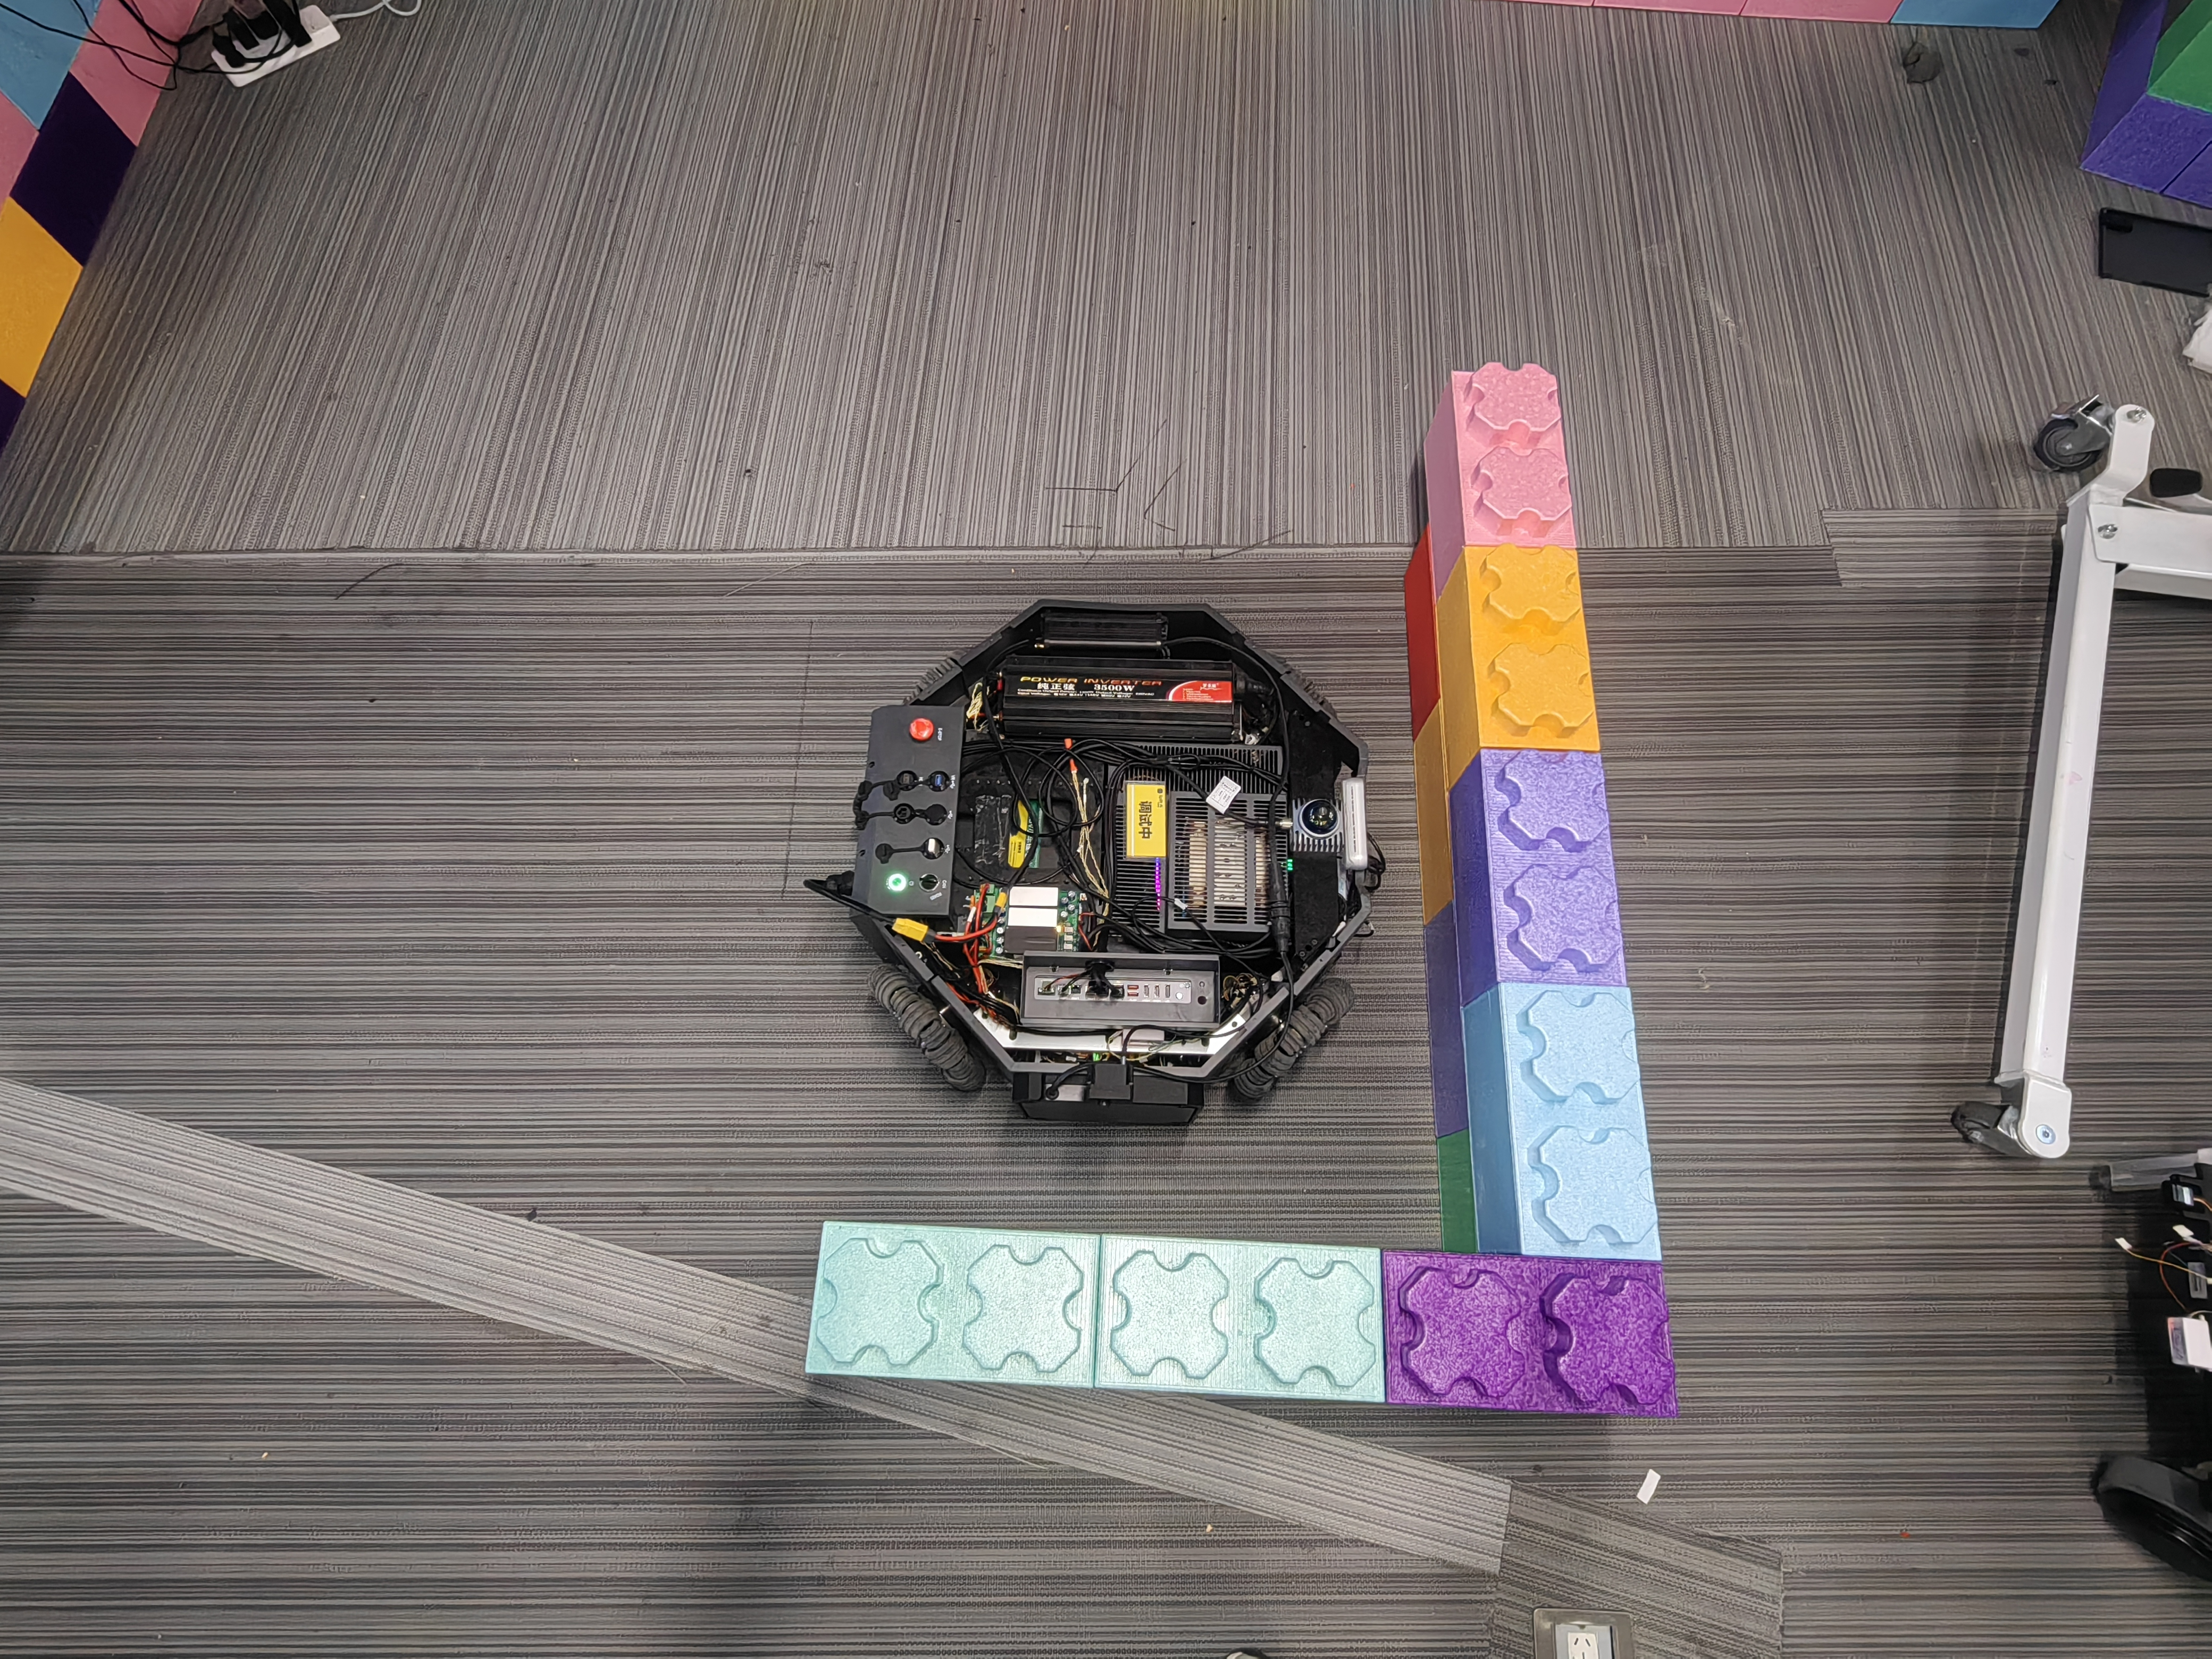
\includegraphics[width=0.48\textwidth]{pic/exp_goal2_neupan.jpg}}
	\caption{实物实验场景与机器人运行状态示例}
	\label{fig:实物实验场景示例}
\end{figure}

\section{L型非凸障碍运行验证}
L型场景将目标区域设置在障碍内凹侧，用于观察点级表示是否能够保留包络内部的真实可行空间。实物验证应以同一场次的ROS日志为准，在统一地图坐标系中叠加真实障碍轮廓、AABB包络、上层参考路径、机器人轨迹和起终点，并同步给出到目标距离、机体系速度及最小障碍距离曲线。现有照片只能证明平台和障碍场景已经搭建，不能替代同条件下的轨迹对照。

\begin{table}[!htb]
	\centering
	\caption{L型实物实验记录表（待同场次日志补充）}
	\label{tab:实物L型结果}
	\scriptsize
	\begin{tabular}{lccccc}
		\toprule
		方法 & 成功次数/总次数 & 终点误差/m & 任务时间/s & 最小距离/m & 平均规划耗时/ms \\
		\midrule
		AABB-MPC & 待填 & 待填 & 待填 & 待填 & 待填 \\
		本文方法 & 待填 & 待填 & 待填 & 待填 & 待填 \\
		\bottomrule
	\end{tabular}
\end{table}

在日志补齐前，本章只保留如下可核验的定性判断：AABB会将L型障碍的内凹部分包含在外接矩形内，因此可能压缩或阻断通向内部目标的可行空间；点级表示在感知边界质量足够时能够避免这一几何误判。是否成功到达、耗时多少以及两种方法差异是否显著，均应由同场次重复实验决定。

\section{复杂障碍环境运行展示与讨论}
多障碍组合照片用于展示规划器在更复杂真实环境中的运行形态。由于当前照片并非同一场景的连续帧，也缺少与AABB-MPC和DWA一一对应的同步日志，本节不据此计算成功率或宣称方法排序。后续若补采数据，应固定场景、起终点和传感器配置，分别运行三种方法，并按与仿真一致的指标生成轨迹与时序图。

真实环境相对仿真环境的主要差异有三点，也是后续补采数据时需重点记录的对象：一是激光雷达点云在障碍侧面与低矮结构上存在缺失，点级约束的有效性直接取决于边界点的完整程度；二是定位输出存在厘米级漂移与短时跳变，会同时影响参考路径截取与距离约束的几何基准；三是底盘存在加速度限制与执行滞后，规划输出的速度指令并非即时生效，可能放大逐次线性化的预测误差。

\section{本章小结}
本章在自研移动机器人平台上对第5章的神经距离编码MPC进行了实物验证部署，明确了传感器配置、定位来源、控制频率和速度指令接口，并说明地图系平移速度经一次平面旋转变换为机体系指令后由麦轮底盘执行，与第5章的建模假设及编码器权重完全一致。针对L型非凸障碍和多障碍组合两类环境，本章给出了实验方案、记录表结构和可核验的定性判断。

当前实物材料仅能证明平台与场景已搭建、软件链路可运行，尚缺少同场次的同步日志，因此本章不给出定量性能结论；所有待填项均须在正式提交前由真实实验日志替换。


\chapter{总结与展望}

\section{工作总结}
本文围绕变电站运维场景下移动机器人自主导航的实际需求，针对复杂环境感知、定位建图、动态障碍物处理以及路径规划等关键问题，开展了面向变电站运维的搬运机器人导航系统设计与实现研究。全文主要工作总结如下：

\begin{enumerate}[label=(\arabic*)]
\item  面向变电站高安全性、高可靠性和复杂空间约束等应用特点，本文分析了运维机器人的功能需求，设计了机器人硬件平台和导航系统总体框架。系统以激光雷达、双目相机等传感器为环境信息输入，结合中央控制模块和底层运动控制模块，为后续环境感知、地图构建、路径规划和运动控制提供了整体实现基础。

\item  针对导航系统中多传感器数据统一表达的问题，本文梳理了世界坐标系、机器人基坐标系、雷达坐标系和相机坐标系之间的转换关系，并介绍了K-Means和DBSCAN等点云聚类基础方法。上述理论为点云处理、障碍物提取和地图构建提供了基础支撑。

\item  针对复杂动态环境中的障碍物感知问题，本文设计了基于深度图像和点云数据融合的轻量级障碍物检测与跟踪方法。该方法结合U深度图检测器和DBSCAN检测器的优势，通过包围盒匹配和融合降低单一传感器噪声带来的误检影响；同时引入基于特征的数据关联、恒加速度模型和点云投票策略，对动态障碍物进行识别与状态估计。在地图构建方面，本文采用局部占用栅格更新，为规划器提供可用于避障决策的环境约束。

\item  针对变电站设备密集、障碍形态复杂且可能存在动态干扰的导航场景，本文设计了全局参考引导与局部滚动优化相结合的路径规划方法。全局层采用目标偏向RRT生成二维拓扑可行参考路径，并通过直连检查、线段碰撞检测、超时处理和路径平滑复检提高工程可用性；局部层构建学习增强MPC方法，在承接障碍物边界和恒加速度状态估计结果的基础上，引入点级障碍表示、动态预测点流和学习型距离特征，降低非凸障碍包络造成的可行空间损失。本文同时完成了规划输出到全向底盘速度接口的设计，使滚动优化得到的首个控制量能够直接转化为机器人可执行指令。
\end{enumerate}

\section{工作展望}
本文围绕变电站运维机器人导航系统的关键模块进行了设计与研究，但距离工程化长期稳定运行仍有进一步完善空间。后续工作可从以下几个方面展开：

\begin{enumerate}[label=(\arabic*)]
\item  进一步完善真实变电站或高保真仿真场景下的系统实验。后续可围绕定位误差、建图精度、障碍物检测准确率、规划耗时、路径平滑性和任务完成率等指标建立更完整的评价体系，并开展多场景、多工况对比实验。

\item  提升复杂电力场景下的多传感器融合鲁棒性。变电站中金属结构密集、电磁环境复杂，单一传感器容易受到遮挡、反射或噪声影响。后续可进一步融合激光雷达、视觉、IMU等多源信息，提高机器人在弱纹理、强反光、遮挡和动态干扰场景下的定位与感知稳定性。

\item  优化动态障碍物预测与局部规划策略。当前方法主要基于显式运动模型和几何约束进行动态避障，后续可结合学习型运动预测、风险场建模或神经规划方法，提高机器人在非凸障碍物、突发动态目标和狭窄通道中的通行能力。

\item  推进导航系统与具体运维任务的深度结合。后续可将导航系统与设备巡检、仪表识别、目标抓取、辅助搬运等任务模块进一步集成，形成从任务分配、路径规划、环境感知到动作执行的闭环作业系统，从而提升变电站机器人系统的实用价值。
\end{enumerate}

% \chapter{大论文撰写技巧}




%%%%%%%%%%%%%%%%%致谢%%%%%%%%%%%%%%%%%%%%%%%%%%%%%%%
 



\acknowledgement
% 致谢



% 在杭州电子科技大学读研的时间过得真的很快，从刚考上杭电的喜悦，初入实验室接触科研学习的不适，后来慢慢熟悉并热爱上自己的研究内容，再到忙碌的找工作和写大论文，这些经历历历在目。在杭电两年半的时间里，我看到了杭电学子务实求学的氛围，以及许多优秀的人在遇到问题时如何解决问题的过程。这段宝贵的经历是我人生中的一大财富，我非常感激杭电！

% 首先，感谢我的导师薛安克老师和葛铭老师在学术道路上的指导和支持，使我在专业领域不断成长。特别感谢我的指导老师郑小青老师，您的耐心指导和鼓励让我在科研过程中不断进步。每一次的组会和讨论，都是我学习和成长的重要一步。感谢我的同届和师兄师弟，你们的支持和陪伴使我的研究之路充满乐趣和动力。我们一起度过了许多难忘的时光，共同面对挑战和收获成果。感谢我的室友黄沈涛、钱越成和汪奇挺，你们在生活和学习中的支持和帮助让我倍感温暖。我们一起分享的点滴时光将成为我美好的回忆。最后，最深切的感谢献给我的父母。感谢你们一直以来的无私支持和无限鼓励。你们的爱和关怀是我前进的动力和坚强后盾。感谢你们的付出，让我能够专心致志地追求自己的学术梦想。


%%%%%%%%%%%%%%%%%%%%%%%%%%%%%%%%%%%%%%%%



%%%%%%%%%%%%%%%%%%%%%%%%%%%%%参考文献%%%%%%%%%%%%%%%%%%%%%%%%%%%%%%%%%
\hdubibliography{ref/reference}
%\bibliographystyle{hdu-thesis}
%\bibliography{ref/reference}
% % %%%%%%%%%%%%%%%%%%%%%%%%%%%%%%%%%%%%%%%%%%%%%%%%%%%%%%%

% %%%%%%%%%%%%%%%%%%%%%%%%%%%%个人成果%%%%%%%%%%%%%%%%%%%%%%%%%%%%%%%
%  %\input{contents/resume}
 \personalresult
 % 张三，男，xxxx年x月生。目前在杭州电子科技大学自动化学院攻读控制科学与工程博士学位。当前研究方向包括自主无人系统等。\\
% {\par\bfseries \noindent 学术论文：}

% [1]***Based on***[J].Neurocomputing(2/4,投稿中)
{\par\bfseries \noindent 期刊论文：}
% [1]一种***方法[P]. 中国，发明专利：\newblock CN1***69A,2023.06.06(1/6,已公开)

[1]Liu, X., Wang, J., Huang, N., Ren, J. (2025, May). A New Privacy-Preserving Mechanism for Networked Agents. In 2025 37th Chinese Control and Decision Conference (CCDC) (pp. 2185-2190). IEEE.(4/4,已见刊)


\par\bfseries \noindent 申请专利：

[1]一种压延设备[P]. CN120461674A,2025.08.12(2/6,已公开)

{\par\bfseries \noindent 竞赛成果：}

[1]“华为杯”第七届中国研究生人工智能创新大赛国家二等奖(4/4)

[2]“兆易创新杯”第二十届中国研究生电子设计大赛华东赛区二等奖(1/3)
{\par\bfseries \noindent 科研项目：}

% [2] 国家自然科学基金委员会，联合基金项目，石化生产过程数字孪生的理论、技术与应用研究，U22A2047，2023-01-01 至 2026-12-31
% [1] 国家自然科学基金重点项目,U2***,***的理论、技术和应用研究,2023~2026




%%%%%%%%%%%%%%%%%%%%%%%%%%%%%%%%%%%%%%%%%%%%%%%%%%%%%%%%%%%%%%%%%%%%%

\end{document}
